\setcounter{section}{10}

\section{Програмування синтаксичних \allowbreak а\-на\-лі\-за\-то\-рів}

\subsection{Синтаксична діаграма}

\textit{Синтаксична діаграма} --- це орієнтований граф, дуги котрого позначені елементами $(N \cup \Sigma)^\star$. Синтаксична діаграма будується для кожного $A$-правила КС-граматики мови програмування. \medskip

Оскільки вершини такого графа не іменуються, то вони припускаються неявно. Синтаксична діаграма позначається іменем нетермінала, для якого вона будується. \medskip

Мета побудови синтаксичних діаграм для мови програмування на основі КС-граматики:
\begin{itemize}
	\item для кожного $A$-правила КС-граматики будується синтаксична діаграма;
	\item на основі побудови синтаксичної діаграми для деякого нетермінала $A \in N$ будуємо підпрограму, яка аналізує ту частину головної програми, яку вона визначає.
\end{itemize}

Оскільки у більшості випадків при визначенні синтаксису мови програмування ми користуємося множиною рекурсивних правил, то серед підпрограм, які будуються на основі правил граматики, будуть і рекурсивні процедури (рекурсія буде як явна, так і неявна). \medskip

Сформулюємо правила побудови синтаксичного графа:
\begin{enumerate}
	\item Кожен нетермінал з відповідною множиною породжуючих правил $A \mapsto \omega_1 \mid \omega_2 \mid \ldots \mid \omega_p$, $\omega_i \in (N \cup \Sigma)^\star$, $i = \overline{1..p}$ відображається в один синтаксичний граф. \medskip

	Отже, кількість синтаксичних графів рівна кількості нетерміналів граматики $G$.

	\item Для кожного елемента слова $\omega = \alpha_1 \alpha_2 \ldots \alpha_p$, $\alpha_i \in (N \cup \Sigma)$, $i = \overline{1..p}$ будуємо ребро синтаксичного графа та покажемо його таким чином що:
	\begin{itemize}
		\item якщо $\alpha_i = x$, $x \in \Sigma$, де $x$ --- вихідна лексема, то будуємо таке ребро:
		\begin{figure}[H]
			\centering
			\begin{tikzpicture}[scale=0.2]
\tikzstyle{every node}+=[inner sep=0pt]
\draw [black] (0,0) circle (3);
\draw [black] (0,0) node {$x$};

\draw [black] (-10,0) -- (-3,0);
\fill [black] (-3,0) -- (-4,-.25) -- (-4,+.25);

\draw [black] (+3,0) -- (+10,0);
\fill [black] (+10,0) -- (+9,-.25) -- (+9,+.25);
\end{tikzpicture}

		\end{figure}

		\item якщо $\alpha_k = A_i \in N$ --- нетермінал граматики, то будуємо таке ребро:
		\begin{figure}[H]
			\centering
			% cd ..\..\Users\NikitaSkybytskyi\Desktop\c3s1\complex-analysis
\documentclass[a4paper, 12pt]{article}
\usepackage[utf8]{inputenc}
\usepackage[english, ukrainian]{babel}

\usepackage{amsmath, amssymb}
\usepackage{multicol}
\usepackage{graphicx}
\usepackage{float}
\usepackage{multicol}

\usepackage{amsthm}
\newtheorem{theorem}{Теорема}[subsection]
\newtheorem*{theorem*}{Теорема}
\newtheorem{lemma}{Лема}[subsection]
\newtheorem*{lemma*}{Лема}
\newtheorem*{remark*}{Зауваження}
\theoremstyle{definition}
\newtheorem*{definition}{Визначення}
\newtheorem{problem}{Задача}[section]
\newtheorem*{solution}{Розв'язок}
\newtheorem{example}{Приклад}
\newtheorem*{example*}{Приклад}
\newtheorem*{hint}{Вказівка}

\newcommand{\Max}{\displaystyle\max\limits}
\newcommand{\Sum}{\displaystyle\sum\limits}
\newcommand{\Int}{\displaystyle\int\limits}
\newcommand{\Lim}{\displaystyle\lim\limits}

\newcommand{\RR}{\mathbb{R}}
\newcommand{\ZZ}{\mathbb{Z}}

\newcommand*\diff{\mathop{}\!\mathrm{d}}
\newcommand*\Diff[1]{\mathop{}\!\mathrm{d^#1}}

\DeclareMathOperator{\Real}{Re}
\DeclareMathOperator{\Imag}{Im}

\DeclareMathOperator{\Arg}{Arg}

\DeclareMathOperator{\Ln}{Ln}

\DeclareMathOperator{\Arctan}{Arctan}
\DeclareMathOperator{\Arcsin}{Arcsin}
\DeclareMathOperator{\Arccos}{Arccos}
\DeclareMathOperator{\Arccosh}{Arccosh}
\DeclareMathOperator{\Arctanh}{Arctanh}

\DeclareMathOperator{\arcsinh}{arcsinh}
\DeclareMathOperator{\arccosh}{arccosh}
\DeclareMathOperator{\arctanh}{arctanh}
\DeclareMathOperator{\arccoth}{arccoth}

\newcommand{\varLimsup}{\varlimsup\limits}

\makeatletter
\newcommand\xLeftrightarrow[2][]{%
  \ext@arrow 9999{\longLeftrightarrowfill@}{#1}{#2}}
\newcommand\longLeftrightarrowfill@{%
  \arrowfill@\Leftarrow\relbar\Rightarrow}
\makeatother

\renewcommand{\epsilon}{\varepsilon}
\renewcommand{\phi}{\varphi}

\allowdisplaybreaks
\setlength\parindent{0pt}
\numberwithin{equation}{subsection}

\usepackage{xcolor}
\usepackage{hyperref}
\hypersetup{unicode=true,colorlinks=true,linktoc=all,linkcolor=red}

\numberwithin{equation}{section}% reset equation counter for sections
\numberwithin{equation}{subsection}
% Omit `.0` in equation numbers for non-existent subsections.
\renewcommand*{\theequation}{%
  \ifnum\value{subsection}=0 %
    \thesection
  \else
    \thesubsection
  \fi
  .\arabic{equation}%
}


\title{{\Huge МАТЕМАТИЧНА ФІЗИКА}}
\author{Скибицький Нікіта}
\date{\today}

\usepackage{amsthm}
\usepackage[dvipsnames]{xcolor}
\usepackage{thmtools}
\usepackage[framemethod=TikZ]{mdframed}

\theoremstyle{definition}
\mdfdefinestyle{mdbluebox}{%
	roundcorner = 10pt,
	linewidth=1pt,
	skipabove=12pt,
	innerbottommargin=9pt,
	skipbelow=2pt,
	nobreak=true,
	linecolor=blue,
	backgroundcolor=TealBlue!5,
}
\declaretheoremstyle[
	headfont=\sffamily\bfseries\color{MidnightBlue},
	mdframed={style=mdbluebox},
	headpunct={\\[3pt]},
	postheadspace={0pt}
]{thmbluebox}

\mdfdefinestyle{mdredbox}{%
	linewidth=0.5pt,
	skipabove=12pt,
	frametitleaboveskip=5pt,
	frametitlebelowskip=0pt,
	skipbelow=2pt,
	frametitlefont=\bfseries,
	innertopmargin=4pt,
	innerbottommargin=8pt,
	nobreak=true,
	linecolor=RawSienna,
	backgroundcolor=Salmon!5,
}
\declaretheoremstyle[
	headfont=\bfseries\color{RawSienna},
	mdframed={style=mdredbox},
	headpunct={\\[3pt]},
	postheadspace={0pt},
]{thmredbox}

\declaretheorem[%
style=thmbluebox,name=Теорема,numberwithin=section]{theorem}
\declaretheorem[style=thmbluebox,name=Лема,sibling=theorem]{lemma}
\declaretheorem[style=thmbluebox,name=Твердження,sibling=theorem]{proposition}
\declaretheorem[style=thmbluebox,name=Наслідок,sibling=theorem]{corollary}
\declaretheorem[style=thmredbox,name=Приклад,sibling=theorem]{example}

\mdfdefinestyle{mdgreenbox}{%
	skipabove=8pt,
	linewidth=2pt,
	rightline=false,
	leftline=true,
	topline=false,
	bottomline=false,
	linecolor=ForestGreen,
	backgroundcolor=ForestGreen!5,
}
\declaretheoremstyle[
	headfont=\bfseries\sffamily\color{ForestGreen!70!black},
	bodyfont=\normalfont,
	spaceabove=2pt,
	spacebelow=1pt,
	mdframed={style=mdgreenbox},
	headpunct={ --- },
]{thmgreenbox}

\mdfdefinestyle{mdblackbox}{%
	skipabove=8pt,
	linewidth=3pt,
	rightline=false,
	leftline=true,
	topline=false,
	bottomline=false,
	linecolor=black,
	backgroundcolor=RedViolet!5!gray!5,
}
\declaretheoremstyle[
	headfont=\bfseries,
	bodyfont=\normalfont\small,
	spaceabove=0pt,
	spacebelow=0pt,
	mdframed={style=mdblackbox}
]{thmblackbox}

% \theoremstyle{theorem}
\declaretheorem[name=Запитання,sibling=theorem,style=thmblackbox]{ques}
\declaretheorem[name=Вправа,sibling=theorem,style=thmblackbox]{exercise}
\declaretheorem[name=Зауваження,sibling=theorem,style=thmgreenbox]{remark}

\theoremstyle{definition}
\newtheorem{claim}[theorem]{Твердження}
\newtheorem{definition}[theorem]{Визначення}
\newtheorem{fact}[theorem]{Факт}

\newtheorem{problem}{Задача}[section]
\renewcommand{\theproblem}{\thesection\Alph{problem}}
\newtheorem{sproblem}[problem]{Задача}
\newtheorem{dproblem}[problem]{Задача}
\renewcommand{\thesproblem}{\theproblem$^{\star}$}
\renewcommand{\thedproblem}{\theproblem$^{\dagger}$}
\newcommand{\listhack}{$\empty$\vspace{-2em}} 

\begin{document}

\tableofcontents

\setcounter{section}{3}

\section{Дослідження граничних задач математичної фізики та методів побудови їх розв'язків}

\subsection{Поняття узагальнених функцій та дії над ними}

Поняття узагальнених функцій виникло як результат природного розширення класичного поняття функції. Так, виконання деяких дій над класичними функціями виводить за межи таких. Вперше узагальнену функцію в математичні дослідження у 1947 році ввів англійський фізик Поль Дірак у своїх квантово-механічних дослідженнях. Така функція отримала назву $\delta$-функція Дірака. Ця функція дозволяє записати просторову щільність фізичної величини (маси, величини заряду, інтенсивності джерела тепла, сили тощо) зосередженої або прикладеної в одній точці. \medskip

Розглянемо приклад, який дає уявлення про $\delta$-функцію. 
\begin{example}
	Нехай $\epsilon$-окіл точки $x$ прямої є джерелом тепла одиничної інтенсивності. Будемо припускати також, що джерело рівномірно розподілене по довжині $\epsilon$-околу. Враховуючи припущення, джерело тепла може бути описане наступною функцією

	\begin{equation}
		f_\epsilon(x) = \begin{cases} 
			0, & x < - \epsilon, \\
			1 / 2 \epsilon, & - \epsilon \le x < \epsilon, \\
			0, & \epsilon \le x.
		\end{cases}
	\end{equation}
\end{example}

\begin{remark}
	При цьому важливо, що сумарна кількість тепла, що виділяється $\epsilon$-околом дорівнює одиниці, тобто
	\begin{equation}
		\Int_{-\infty}^\infty f_\epsilon(x) \diff x = 1.
	\end{equation}
\end{remark}
Припустимо, що фізичний розмір джерела такий малий, що його розмірами можна нехтувати, тобто будемо вважати що джерело є точковим. \medskip

В цьому випадку природно визначити функцію 
\begin{equation}
	f_0(x) = \Lim_{\epsilon \to 0} f_\epsilon(x) = \begin{cases}
		0, & x \ne 0, \\
		\infty, & x = 0.
	\end{cases}
\end{equation}

Легко бачити, що інтеграл Лебега функції $f_0(x)$ існує і дорівнює нулю:
\begin{equation}
	\Int_{-\infty}^\infty f_0(x) \diff x = 0.
\end{equation}

Тобто користуючись звичайним граничним переходом (поточковою границею) ми отримуємо функцію, яка не моделює одиничне точкове джерело тепла. \medskip

Для коректного визначення граничної функції будемо розглядати замість сильної (поточкової) границі, слабку границю. \medskip

Введемо набір пробних функцій $D(\RR^n) = C_\infty^0 (\RR^n)$ --- множину нескінченно диференційовних в $\RR^n$ функцій з компактним носієм. 

\begin{remark}
	Нагадаємо, що функція має компактний носій якщо існує куля $U_A(0)$ радіусу $A$, за межами якої функція обертається в тотожній нуль разом з усіма своїми похідними.
\end{remark}

\begin{proposition}
	Виконується рівність
	\begin{equation}
		\Lim_{\epsilon \to 0} \Int_{-\infty}^\infty f_\epsilon(x) \phi(x) \diff x = \phi(0)
	\end{equation}	
	для довільної $\phi \in D(\RR^1)$.
\end{proposition}

\begin{proof}
	Справді:
	\begin{equation}
		\begin{aligned}
			\left| \Int_{-\infty}^\infty f_\epsilon(x) \phi(x) \diff x - \phi(0) \right| &= \left| \Int_{-\infty}^\infty f_\epsilon(x) (\phi(x) - \phi(0)) \diff x \right| \le \\
			&\le \frac{1}{2\epsilon} \Int_\epsilon^\epsilon |\phi(x) - \phi(0)| \diff x = \\
			&= \frac{\eta(\epsilon)}{2\epsilon} \Int_\epsilon^\epsilon \diff x = \eta(\epsilon) \xrightarrow[\epsilon \to 0]{} 0.
		\end{aligned}	
	\end{equation}

	Це означає, що слабка границя дорівнює $\phi(0)$ для довільної $\phi \in D(\RR^1)$.
\end{proof}
	
\begin{remark}
	Тут ми винесли середнє значення підінтегралньої функції $g(x) = |\phi(x) - \phi(0)|$ з-під інтегралу, тобто $\eta(\epsilon) = g(\xi) = |\phi(\xi) - \phi(0)|$, де $\xi = \xi(\epsilon)$ --- якась середня точка, $\xi \in (-\epsilon, \epsilon)$. \medskip

	Далі, $|\phi(\xi) - \phi(0)| \to 0$ при $\xi \to 0$, а $\xi \to 0$ при $\epsilon \to 0$ бо $|\xi| < |\epsilon|$. \medskip

	Нарешті, $\eta(\epsilon) \to 0$ при $\epsilon \to 0$ адже $\phi$ --- неперервна, тобто $|\phi(\xi) - \phi(0)| \to 0$ при $\xi \to 0$, і знову-ж-таки $\xi \to 0$ при $\epsilon \to 0$ бо $|\xi| < |\epsilon|$.
\end{remark}

Таким чином $\delta$-функцію Дірака можна визначити, як слабку границю послідовності функції $f_\epsilon$ на множині $D(\RR^1)$, що збігається до числа $\phi(0)$ при $\epsilon \to 0$. \medskip

Можна записати 
\begin{equation}
	\Lim_{\epsilon \to 0} \Int_{-\infty}^\infty f_\epsilon(x) \phi(x) \diff x = \Int_{-\infty}^\infty \delta(x) \phi(x) \diff x.
\end{equation}

Останню рівність будемо розглядати як лінійний неперервний функціонал, який будь-якій функції $\phi$ ставить у відповідність число $\phi(0)$.

\begin{definition}[узагальненої функції]
	\it{Узагальненою функцією} $f$ будемо називати будь-який лінійний неперервний функціонал   заданий на множині основних (пробних) функцій $\phi \in D(\RR^n)$.
\end{definition}

\begin{remark}
	Лінійність і неперервність розуміємо в традиційному сенсі:
	\begin{equation}
		\langle f, a_1 \phi_1 + a_2 \phi_2 \rangle = a_1 \langle f, \phi_1 \rangle + a_2 \langle f, \phi_2 \rangle,
	\end{equation}
	і
	\begin{equation}
		\Lim_{k \to \infty} \langle f, \phi_k \rangle = 0,
	\end{equation}
	для довільної $\{\phi_k\}_{k = 1}^\infty$ такої, що $D^{\alpha_1 \ldots \alpha_n} \phi_k(x) \xrightarrow[k \to \infty]{} 0$ для довільних $\alpha_1, \ldots, \alpha_n$.
\end{remark}

Серед усіх узагальнених функцій виділяють клас регулярних узагальнених функцій.
\begin{definition}[регулярної функції]
	\it{Регулярними} називаються функції, які можуть бути представлені у вигляді 
	\begin{equation}
		\phi \mapsto \langle f, \phi \rangle = \Iiint_{\RR^n} f(x) \phi(x) \diff x
	\end{equation}
	з функцією $f(x) \in L_{\text{loc}}^1$ --- тобто абсолютно інтегровною функцією на будь-якому компакті, що належить $\RR^n$.
\end{definition}

\begin{remark}
	Кожна локально інтегрована функція визначає \it{єдину} регулярну узагальнену функцію і навпаки, кожна регулярна узагальнена функція визначає \it{єдину} локально інтегровану функцію. 
\end{remark}

\begin{remark}
	\it{Єдиність} означає, що дві локально інтегровані функції співпадають якщо вони відрізняються між собою на множині нульової міри.
\end{remark}

\begin{definition}[сингулярної функції]
	Усі інші лінійні неперервні функціонали визначають \it{сингулярні} узагальнені функції.
\end{definition}

\begin{example}[сингулярної функції]
	$\delta$-функція Дірака.
\end{example}

\begin{remark}
	Дуже часто узагальнені функції називають також \it{розподілами}.
\end{remark}

Хоча сингулярні узагальнені функції є частинним випадком узагальнених функцій, але для їх представлення найчастіше використовується позначення скалярного добутку таке саме як і для регулярних узагальнених функцій. \medskip

Справа в тому, що 
\begin{proposition}
	Для будь-якої сингулярної узагальненої функції $f: \phi \mapsto \langle f, \phi \rangle$ можна побудувати послідовність регулярних узагальнених функцій, яка слабко збігається до неї, тобто $\exists \{f_k\}_{k = 1}^\infty$, $f_k \in L_{\text{loc}}^1(\RR^n)$ така, що
	\begin{equation}
		\Lim_{k \to \infty} \Iiint_{\RR^n} f_k(x) \phi(x) \diff x = \langle f, \phi \rangle
	\end{equation}
\end{proposition}

\begin{remark}
	Ця послідовність не єдина.
\end{remark}

\begin{remark}
	$\delta$-функцію ми побудували як границю $\Lim_{\epsilon \to 0} f_\epsilon$, яку можна було назвати \it{$\delta$-образною} послідовністю.
\end{remark}

Можна навести і інші
\begin{examples}[$\delta$-образних послідовностей]
	$\delta$-образними послідовностями також є:
	\begin{itemize}
		\item $f_m(x) = \dfrac{m}{\pi (1 + m^2 x^2)}$;
		\item $f_m(x) = \dfrac{\sin m x}{\pi x}$;
		\item $f_m(x) = \dfrac{m}{\sqrt{2 \pi}} \exp \left\{ - \dfrac{m^2 x^2}{2}\right\}$.
	\end{itemize}
\end{examples}

\begin{remark}
	Константи у знаменниках тут для того, щоби
	\begin{equation}
		\Int_{-\infty}^\infty f_m(x) \diff x = 1.
	\end{equation}
\end{remark}
 	  		 
\subsubsection{Узагальнені функції та фізичні розподіли}

Узагальнені функції (часто їх називають розподілами) можна інтерпретувати як розподіл електричних, магнітних зарядів або розподіл мас, тощо. Так наприклад функцію Дірака можна трактувати як щільність з якою розподілена маса, що дорівнює одиниці в точці $x = 0$. 

\begin{definition}[зсунутої $\delta$-функції]
	Аналогічним чином можна ввести і зсунуту функцію Дірака.
	\begin{equation}
		\Int_{-\infty}^\infty \delta(x - a) \phi(x) \diff x = \phi(a).
	\end{equation}
\end{definition}

\begin{remark}
	Використовуючи цю формулу можна зобразити щільність розподілу зосереджених мас або іншої фізичної величини в точках прямої.
\end{remark}

\begin{example}
	Так, якщо в точках $x_i$ розташовані зосереджені маси $m_i$, $i \in I$, то
	щільність такого розподілу мас можна зобразити у вигляді
	\begin{equation}
		\rho(x) = \Sum_{i \in I} m_i \cdot \delta(x - x_i).	
	\end{equation}
\end{example}

\begin{remark}
	При цьому повну масу, яка зосереджена на прямій можна порахувати за формулою
	\begin{equation}
		\Int_{-\infty}^\infty \rho(x) \diff x = \Sum_{i \in I} m_i.	
	\end{equation}
\end{remark}

\begin{definition}[$\delta$-функції в $\RR^n$]
	Аналогічно $\delta$-функції, введеній на прямій, можна ввести $\delta$-функцію для $n$-вимірного евклідового простору:
	\begin{equation}
		\Iiint_{\RR^n} \delta(x - a) \phi(x) \diff x = \phi(a).
	\end{equation}
\end{definition}

\begin{remark}
	Тоді щільність розподілу точкових мас у просторі можна також записати у вигляді
	\begin{equation}
		\rho(x) = \Sum_{i \in I} m_i \cdot \delta_3(x - x_i).	
	\end{equation}
\end{remark}

Нагадаємо
\begin{proposition}
	Точковий одиничний електричний заряд розташований в точці $x_0$ створює потенціал рівний
	\begin{equation}
		\Iiint_{\RR^3} \frac{\delta(y - x_0) \diff y}{4 \pi |x - y|} = \frac{1}{4 \pi |x - x_0|}
	\end{equation}
	в точці $x \in \RR^3$. 
\end{proposition}

\begin{remark}
	В цьому випадку $\delta(y - x_0)$ можна сприймати як щільність одиничного точкового заряду.
\end{remark}

\begin{example}
	Якщо щільність зарядів $f(y)$ представляє собою локально інтегровану функцію, то маємо для потенціалу електростатичного поля відому формулу електростатики:
	\begin{equation}
		P(x) = \Iiint_{\RR^3} \frac{f(x) \diff y}{4 \pi |x - y|}.	
	\end{equation}
\end{example}

\begin{definition}[поверхневої функції Дірака]
	Узагальненням точкової функції Дірака є так звана \it{поверхнева функція Дірака} $\delta_S$, яку можна визначити як лінійний неперервний функціонал:
	\begin{equation}
		\phi \mapsto \langle \delta_S, \phi \rangle = \Iint_{S} \phi(x) \diff x.	
	\end{equation}
\end{definition}

\begin{remark}
	Ця узагальнена функція може бути інтерпретована як щільність розподілу зарядів на поверхні $S$.
\end{remark}

\begin{example}
	Потенціал електростатичного поля можна записати у вигляді
	\begin{equation}
		W(x) = \langle \mu(y) \delta_S(y), \frac{1}{4 \pi |x - y|} \rangle = \Iiint_{\RR^3} \frac{\mu(y) \delta_S(y) \diff y}{4 \pi |x - y|} = \Iint_{S} \frac{\mu(y) \diff y}{4 \pi |x - y|}.	
	\end{equation}
\end{example}

\begin{definition}[потенціалу просторого шару]
	Легко бачити, що $W(x)$ представляє собою потенціал електростатичного поля, утворений зарядженою поверхнею $S$ і називається \it{потенціалом простого шару}.
\end{definition}

\subsubsection{Дії над узагальненими функціями}

Головною перевагою узагальнених функцій є те, що будь-яка узагальнена функція має похідні будь-якого порядку. \medskip

Для визначення похідної узагальненої функції розглянемо звичайну неперервно диференційовну функцію $f(x)$ і згадаємо, що виконується наступна
\begin{th_formula}[інтегрування за частинами]
	\begin{equation}
		\Int_{\RR^n} D^{\alpha_1 \ldots \alpha_n} f(x) \phi(x) \diff x = (-1)^{|\alpha|} \Int_{\RR^n} f(x) D^{\alpha_1 \ldots \alpha_n} \phi(x) \diff x,
	\end{equation}
	де $|\alpha| = \alpha_1 + \ldots + \alpha_n$, яка є істинною для будь-якої функції $\phi \in D(\RR^n)$.
\end{th_formula}

Права частина цієї рівності має зміст для будь-якої локально-інтегровної функції $f$. \medskip \allowbreak

Таким чином можемо дати
\begin{definition}[похідної локально-інтегровної функції]
	\it{Похідною} $D^{\alpha_1 \ldots \alpha_n}$ будь-якої локально-інтегровної функції $f$ будемо називати лінійний неперервний функціонал
	\begin{equation}
		\langle D^{\alpha_1 \ldots \alpha_n} f, \phi \rangle = (-1)^{|\alpha|} \Int_{\RR^n} f(x) D^{\alpha_1 \ldots \alpha_n} \phi(x) \diff x.	
	\end{equation}
\end{definition}

Аналогічним чином вводиться похідна і для сингулярних узагальнених функцій.
\begin{definition}[похідної сингулярних функцій]
	$D^{\alpha_1 \ldots \alpha_n} f$ визначається як лінійний неперервний функціонал
	\begin{equation}
		\langle D^{\alpha_1 \ldots \alpha_n} f, \phi \rangle = (-1)^{|\alpha|} \langle f, D^{\alpha_1 \ldots \alpha_n} \phi \rangle.
	\end{equation}
\end{definition}

Розглянемо приклади обчислення похідних деяких узагальнених функцій:
\begin{example}
	Знайти $\theta'$, де 
	\begin{equation}
		\theta(x) = \begin{cases}
			0, & x \le 0, \\
			1, & 0 < x
		\end{cases}	
	\end{equation}
	--- функція Хевісайда.
\end{example}

\begin{solution}
	Розглянемо наступні рівності:
	\begin{equation}
		\begin{aligned}
			\langle \theta', \phi \rangle &= - \Int_{-\infty}^\infty \theta(x) \phi'(x) \diff x = - \Int_{0}^\infty \phi'(x) \diff x = \\
			&= - (\phi(\infty) - \phi(0)) = \phi(0) - \phi(\infty) = \phi(0) - 0 = \phi(0) = \langle \delta, \phi \rangle.	
		\end{aligned}
	\end{equation}

	Таким чином можна записати $\theta' = \delta$.
\end{solution}

\begin{example}
	Знайти $\delta^{(2)}$.
\end{example}

\begin{solution}
	\begin{equation}
		\langle \delta^{(2)}, \phi \rangle = \langle \delta, \phi^{(2)} \rangle = \phi^{(2)}(0).
	\end{equation}
\end{solution}

\begin{example}
	$f$ --- кусково неперервно-диференційовна функція, яка має в деякій точці $x_0$ розрив першого роду.
\end{example}

\begin{solution}
	\begin{equation}
		\begin{aligned}
			\langle f', \phi \rangle &= - \Int_{-\infty}^\infty f(x) \phi'(x) \diff x = \\
			&= - \Int_{-\infty}^{x_0} f(x) \phi'(x) \diff x -\Int_{x_0}^\infty f(x) \phi'(x) \diff x = \\
			&= - f(x_0 - 0) + \phi(x_0) + f(x_0 + 0) \phi(x_0) + \\
			&\quad + \Int_{-\infty}^{x_0} f(x)' \phi(x) \diff x + \Int_{x_0}^\infty f(x)' \phi(x) \diff x = \\
			&= \phi(x_0) [f(x_0)] + \Int_{-\infty}^{x_0} f(x)' \phi(x) \diff x + \Int_{x_0}^\infty f(x)' \phi(x) \diff x = \\
			&= \phi(x_0) [f(x_0)] + \Int_{-\infty}^\infty f(x)' \diff x  = \\
			&= \Int_{-\infty}^\infty \Big( [f(x_0)] \cdot \delta(x - x_0) + \{f(x)'\} \Big) \phi(x) \diff x,
		\end{aligned}
	\end{equation}
	де $[f(x_0)] = f(x_0 + 0) - f(x_0 - 0)$, $\{f'(x)\}$ --- локально інтегрована функція, яка співпадає з звичайною похідною функції $f$ в усіх точках де вона існує.
\end{solution}

\begin{remark}
	Таким чином для функції, яка має скінчену кількість точок розриву першого роду має місце така формула обчислення похідної:
	\begin{equation}
		f'(x) = \{f'(x)\} + \Sum_{i} [f(x_i)] \delta (x - x_i).
	\end{equation}
\end{remark}

\begin{example}
	Нехай функція $f(x)$ задана в просторі $\RR^3$ кусково неперервно-ди\-фе\-рен\-ці\-йов\-на і має розрив першого роду на кусково–гладкій поверхні $S$. Будемо припускати, що поверхня   розділяє простір $\RR^3$ на два півпростори $\RR_+^3$ та $\RR_-^3$.
\end{example}

\begin{solution}
	Зафіксуємо на $S$ напрям нормалі, яка направлена всередину $\RR_+^3$. \medskip

	Визначимо похідну від $f(x)$:
	\begin{equation}
		\begin{aligned}
			\langle \frac{\partial f}{\partial x_i}, \phi \rangle &= - \Iiint_{\RR^3} f(x) \frac{\partial \phi(x)}{\partial x_i} \diff x = \\
			&= - \Iiint_{\RR_+^3} f(x) \frac{\partial \phi(x)}{\partial x_i} \diff x - \Iiint_{\RR_-^3} f(x) \frac{\partial \phi(x)}{\partial x_i} \diff x = \\
			&= \Iint_S f(x + 0) \phi(x) \cos(n, x_i) \diff S - \\
			&\quad- \Iint_S f(x - 0) \phi(x) \cos(n, x_i) \diff S + \\
			&\quad + \Iiint_{\RR_+^3} \phi(x) \frac{\partial f(x)}{\partial x_i} \diff x + \Iiint_{\RR_-^3} \phi(x) \frac{\partial f(x)}{\partial x_i} \diff x = \\
			&= \Iiint_{\RR^3} \left(  \left\{ \frac{\partial f}{\partial x_i}\right\} + [f]_S(x) \cos(n, x_i) \right) \phi(x) \diff x.
		\end{aligned}	
	\end{equation}
	де $\{\partial f(x) / \partial x_i\}$ --- класична похідна функції $f(x)$ в усіх точках, де вона існує, $[f(x)]_S = \left.(f(x + 0) - f(x - 0))\right|_{x \in S}$ --- стрибок функції $f(x)$ на поверхні $S$. \medskip

	Таким чином можна записати, що 
	\begin{equation}
		\frac{\partial f}{\partial x_i} = \left\{ \frac{\partial f}{\partial x_i}\right\} + [f]_S(x) \cos(n, x_i) \delta_S(x).
	\end{equation}
\end{solution}

\subsubsection{Носій та порядок узагальнених функцій}

Вводячи поняття узагальнених функцій ми використовували множину основних (пробних) функцій $D(\RR^n) = C_\infty^0(\RR^n)$. Взагалі кажучи, простір пробних функцій (а таким чином і розподілів) можна узагальнити, ввівши простір основних функцій як $D(\Omega) = C_\infty^0(\Omega)$, тобто клас пробних функцій складається з функцій, які нескінченно-диференційовні в $\Omega$ і на границі $\partial \Omega$ перетворюються в нуль разом з усіма своїми похідними. \medskip

Для побудови функцій такого класу використовуються $\epsilon$-шапочки.

\begin{definition}[$\epsilon$-шапочки]
	$\epsilon$-шапочкою називається функція
	\begin{equation}
		\omega_\epsilon(x) = \begin{cases}
			C_\epsilon \exp \left\{ - \frac{\epsilon^2}{\epsilon^2 - |x|^2} \right\}, & |x| \le \epsilon, \\
			0, & |x| > \epsilon.
		\end{cases}
	\end{equation}
\end{definition}

\begin{remark}
	Сталу $C_\epsilon$ обираємо так, щоби 
	\begin{equation}
		\Iiint_{\RR^n} \omega_\epsilon (x) \diff x = 1.
	\end{equation}
\end{remark}

Легко бачити, що 
\begin{equation}
	\Lim_{\epsilon \to +0} \Iiint_{\RR^n} \omega_\epsilon(x - y) \phi(y) \diff y = \phi(x).
\end{equation}

Це означає, що $\epsilon$-шапочки слабко збігаються до $\delta(x)$ при $\epsilon \to + 0$. \medskip

Введемо функцію
\begin{equation}
	\eta(x) = \Iiint_{\RR^n} \chi(x) \omega_\epsilon(x - y) \diff y,
\end{equation}
де $\chi(x)$ -- характеристична функція множини $\Omega_{2\epsilon}$, тобто
\begin{equation}
	\chi(x) = \begin{cases}
		1, & x \in \Omega_{2 \epsilon}, \\
		0, & x \notin \Omega_{2 \epsilon}, 
	\end{cases}
\end{equation}
а множина $\Omega_{2 \epsilon}$ утворилася з множини $\Omega$ шляхом відступу всередину $\Omega$ від границі на полосу ширини $2 \epsilon$. \medskip

Тоді будь-яка функція $\phi(x) = \eta(x) f(x) \in D(\Omega)$ якщо $f(x) \in C^\infty(\RR^n)$. \medskip

Таким чином можна утворити достатньо широкий клас пробних функцій.
\begin{remark}
	Узагальнені функції взагалі кажучи не мають значень в окремих точках. \medskip

	В той же час можна говорити про обертання узагальненої функції на нуль у деякій області.
\end{remark}

\begin{definition}[обертання узагальненої функції на нуль]
	Будемо говорити, що узагальнена функція $f$ \it{обертається на нуль} у області $\Omega$, якщо $\langle f, \varphi \rangle = 0$, $\forall \varphi \in D(\Omega)$.
\end{definition} 

\begin{definition}[нульової множини узагальненої функції]
	\it{Нульовою множиною} $O_f$ узагальненої функції $f$ будемо називати об'єднання усіх областей у яких узагальнена функція $f$ обертається на нуль. 
\end{definition}

\begin{definition}[носія узагальненої функції]
	\it{Носієм} $\text{supp} f$ узагальненої функції $f$ називають множину $\RR^n \setminus O_f$.
\end{definition}

\begin{definition}[порядку узагальненої функції]
	Будемо говорити, що узагальнена функція $f$ має \it{порядок сингулярності} (або просто порядок) $\le j$, якщо
	\begin{equation}
		f = \Sum_{|\alpha| \le j} D^\alpha g_\alpha,	
	\end{equation}
	де $g_\alpha \in L_{\text{loc}}^1 (\Omega)$. Якщо число $j$ у цій формулі неможливо зменшити, то кажуть що порядок узагальненої функції $f$ \it{дорівнює} $j$.
\end{definition}

Нехай $f$ --- узагальнена функція порядку $j$, а $\phi$ --- довільна пробна функція. За визначенням
\begin{equation}
	\langle f, \phi \rangle = \Sum_{|\alpha| \le j} \langle D^\alpha g_\alpha, \phi \rangle = \Sum_{|\alpha| \le j} (-1)^{|\alpha|} \Iiint_\Omega g_\alpha D^\alpha \phi \diff x, \quad \forall \phi \in D(\Omega).
\end{equation}

Неважко бачити, що права частина цієї формули зберігає зміст не тільки для функцій з класу $D(\Omega)$, але і для функцій ширшого класу $D^j(\Omega)$.

\begin{remark}
	Узагальнені функції порядку $j$ можна визначати як лінійні неперервні функціонали на класі основних функцій $D^j(\Omega)$.
\end{remark}



\subsubsection{Згортка та регуляризація узагальнених функцій}

Нехай $f(x), g(x)$ --- дві локально-інтегровні функції в $\RR^n$. При цьому функція 
\begin{equation}
	h(x) = \Iiint_{\RR^n} | g(y) f(x - y) | \diff y	
\end{equation}
теж буде локально-інтегровна в $\RR^n$. 

\begin{definition}[згортки]
	\it{Згорткою} $f * g$ цих функцій будемо називати функцію
	\begin{equation}
		(f * g) (x) = \Iiint_{\RR^n} f(y) g(x - y) \diff y =  \Iiint_{\RR^n} g(y) f(x - y) \diff y = (g * f)(x).		
	\end{equation}
\end{definition}

Таким чином згортка є локально-інтегровною функцію і тим самим визначає регулярну узагальнену функцію, яка діє на основні функції за правилом
\begin{equation}
	\varphi \mapsto \Iiint_{\RR^n} (f * g) (\xi) \varphi(\xi) \diff \xi.	
\end{equation}

Розглянемо випадок згортки двох функцій $f$ та $\psi$, де $f$ --- узагальнена, а $\psi$ --- основна (пробна) функція. Оскільки $\psi$ --- фінітна функція, то згортка $f * \psi$ існує, а враховуючи нескінчену гладкість пробної функції, $(f * \psi) \in C^\infty(\RR^n)$.

\begin{definition}
	\it{Регуляризацією} узагальненої функції $f$ будемо називати функцію $f_\epsilon = f * \omega_\epsilon$.
\end{definition}

Зрозуміло, що $f_\epsilon \in C^\infty (\RR^n)$, а враховуючи властивості $\epsilon$-шапочки $\omega_\epsilon$ легко бачити, що 
\begin{equation}
	f_\epsilon \xrightarrow[\epsilon \to 0]{\text{w.}} f,
\end{equation}
тобто довели
\begin{proposition}
	Будь-яка узагальнена функція є слабка границя своїх регуляризацій.
\end{proposition}

\begin{example}
	Розглянемо узагальнену функцію
	\begin{equation}
		P \frac{1}{x - a},
	\end{equation}
	яка співпадає на усій числовій прямій з функцією $\frac{1}{x - a}$ за винятком точки $a$ і визначає лінійний неперервний функціонал, який діє за правилом
	\begin{equation}
		\begin{aligned}
			\langle P \frac{1}{x - a}, \psi \rangle &= \text{v.p.} \Int_{-\infty}^\infty \frac{\psi(x)}{x - a} \diff x = \\
			&= \Lim_{\epsilon \to 0} \left( \Int_{-\infty}^{a - \epsilon}\frac{\psi(x)}{x - a} \diff x + \Int_{a + \epsilon}^\infty \frac{\psi(x)}{x - a} \diff x \right).
		\end{aligned}
	\end{equation}

	Розглянемо узагальнену функцію
	\begin{equation}
		P \frac{1}{(x - a)^2},
	\end{equation}
	яка співпадає на усій числовій прямій з функцією $\frac{1}{(x - a)^2}$ за винятком точки $a$ і визначає лінійний неперервний функціонал, який діє за правилом
	\begin{equation}
		\begin{aligned}
			\langle P \frac{1}{(x - a)^2}, \psi \rangle &= \text{v.p.} \Int_{-\infty}^\infty \frac{\psi(x) - \psi(a)}{(x - a)^2} \diff x = \\
			&= \Lim_{\epsilon \to 0} \left( \Int_{-\infty}^{a - \epsilon}\frac{\psi(x) - \psi(a)}{(x - a)^2} \diff x + \Int_{a + \epsilon}^\infty \frac{\psi(x) - \psi(a)}{(x - a)^2} \diff x \right).
		\end{aligned}
	\end{equation}

	Покажемо, що 
	\begin{equation}
		\left( P \frac{1}{x - a} \right)' = P \frac{1}{(x - a)^2}
	\end{equation}
	з точки зору узагальнених функцій.
\end{example}

\begin{proof}
	Справді,
	\begin{equation}
		\begin{aligned}
			\langle \left( P \frac{1}{x - a} \right)', \psi \rangle &= - \langle P \frac{1}{x - a}, \psi' \rangle = \\
			&= - \Lim_{\epsilon \to 0} \left( \Int_{-\infty}^{a - \epsilon}\frac{\psi'(x)}{x - a} \diff x + \Int_{a + \epsilon}^\infty \frac{\psi'(x)}{x - a} \diff x \right) = \\
			&= - \Lim_{\epsilon \to 0} \left( \Int_{-\infty}^{a - \epsilon}\frac{\diff (\psi(x) - \psi(a))}{x - a} + \Int_{a + \epsilon}^\infty \frac{\diff (\psi(x) - \psi(a))}{x - a} \right) = \\
			&= - \Lim_{\epsilon \to 0} \left( \left. \frac{\psi(x) - \psi(a)}{x - a} \right|_{-\infty}^{a - \epsilon} + \left. \frac{\psi(x) - \psi(a)}{x - a}\right|_{a + \epsilon}^\infty \right. + \\
			&\quad + \left. \Int_{-\infty}^{a - \epsilon}\frac{\psi(x) - \psi(a)}{(x - a)^2} \diff x + \Int_{a + \epsilon}^\infty \frac{\psi(x) - \psi(a)}{(x - a)^2} \diff x \right) = \\
			&= - \Lim_{\epsilon \to 0} \left( \Int_{-\infty}^{a - \epsilon}\frac{\psi(x) - \psi(a)}{(x - a)^2} \diff x + \Int_{a + \epsilon}^\infty \frac{\psi(x) - \psi(a)}{(x - a)^2} \diff x \right) - \\
			&\quad-\Lim_{\epsilon \to 0} \left( \frac{\psi(a - \epsilon) - \psi(a)}{-\epsilon} - \frac{\psi(a + \epsilon) - \psi(a)}{\epsilon} \right) = \\
			&= -\text{v.p.} \Int_{-\infty}^\infty \frac{\psi(x) - \psi(a)}{(x - a)^2} \diff x = - \langle P \frac{1}{(x - a)^2}, \psi \rangle.
		\end{aligned}
	\end{equation}
\end{proof}

\newpage

\end{document}
		\end{figure}
	\end{itemize}
\end{enumerate}

Тоді, коли правило граматики $G$ має вигляд $A_i \mapsto \alpha_1 A_1 \ldots$ для побудови діаграми скористаємося обома способами:
\begin{figure}[H]
	\centering
	\begin{tikzpicture}[scale=0.2]
\tikzstyle{every node}+=[inner sep=0pt]
\draw [black] (-20,0) -- (-13,0);
\fill [black] (-13,0) -- (-14,-.25) -- (-14,+.25);

\draw [black] (-10,0) circle (3);
\draw [black] (-10,0) node {$\alpha_1$};

\draw [black] (-7,0) -- (-2.5,0);
\fill [black] (-2.5,0) -- (-3.5,-.25) -- (-3.5,+.25);

\draw [black] (-2.5,-2.5) -- (-2.5,+2.5) -- (+2.5,+2.5) -- (+2.5,-2.5) -- cycle;
\draw [black] (0,0) node {$A_1$};

\draw [black] (+2.5,0) -- (+10,0);
\fill [black] (+10,0) -- (+9,-.25) -- (+9,+.25);

\draw [black] (+12,0) node {$\ldots$};
\end{tikzpicture}

\end{figure}

Коли правило граматики $G$ має вигляд $A_i \mapsto \omega_1 \mid \omega_2 \mid \ldots \mid \omega_p$, то відповідний синтаксичний граф буде мати вигляд:
\begin{figure}[H]
	\centering
	\begin{tikzpicture}[scale=0.2]
\tikzstyle{every node}+=[inner sep=0pt]
\draw [black] (-20,+5) -- (-10,+5);
\fill [black] (-10,+5) -- (-11,+4.75) -- (-11,+5.25);

\fill [black] (-10,-15) -- (-9.75,-14) -- (-10.25,-14);
\draw [black] (-10,+5) -- (-10,-15);

\draw [black] (-10,0) -- (-1,0);
\fill [black] (-1,0) -- (-2,-.25) -- (-2,+.25);
\draw [black] (0,0) node {$\omega_1$};
\fill [black] (+10,0) -- (+9,-.25) -- (+9,+.25);
\draw [black] (+1,0) -- (+10,0);

\draw [black] (-10,-5) -- (-1,-5);
\fill [black] (-1,-5) -- (-2,-5.25) -- (-2,-4.75);
\draw [black] (0,-5) node {$\omega_2$};
\fill [black] (+10,-5) -- (+9,-5.25) -- (+9,-4.75);
\draw [black] (+1,-5) -- (+10,-5);

\draw [black] (0,-10) node {$\vdots$};

\draw [black] (-10,-15) -- (-1,-15);
\fill [black] (-1,-15) -- (-2,-15.25) -- (-2,-14.75);
\draw [black] (0,-15) node {$\omega_p$};
\fill [black] (+10,-15) -- (+9,-15.25) -- (+9,-14.75);
\draw [black] (+1,-15) -- (+10,-15);

\fill [black] (+10,+5) -- (+9.75,+4) -- (+10.25,+4);
\draw [black] (+10,-15) -- (+10,+5);

\draw [black] (+20,+5) -- (+10,+5);
\fill [black] (+20,+5) -- (+19,+4.75) -- (+19,+5.25);
\end{tikzpicture}

\end{figure}
де замість $\omega_1, \omega_2, \ldots, \omega_p$ будуються відповідні синтаксичні діаграми. \medskip

Якщо на основі граматики мови програмування побудована множина синтаксичних графів, то можна спробувати зменшити їх кількість, скориставшись підстановкою одних графів у інші. При цьому замість елемента $A_i$ підставляється його синтаксичний граф. Таким чином можна зменшити кількість синтаксичних графів. Для того, щоб забезпечити детермінований синтаксичний аналіз з переглядом вперед на одну лексему, потрібно накласти певні обмеження, а саме: для кожного правила $A_i$ виду  $A_i \mapsto \omega_1 \mid \omega_2 \mid \ldots \mid \omega_p$ з синтаксичною діаграмою наведеного вище вигляду необхідне виконання наступної умови: множини $\text{First}_1(\omega_j) \oplus_1 \text{Follow}_1 (A_i)$, $j = \overline{1..p}$ повинні попарно не перетинатися. Зрозуміло, що ця умова гарантує детермінований вибір шляху при русі по синтаксичній діаграмі.

\subsubsection{Код}

Подальше програмування синтаксичного аналізатора можна звести до наступних примітивів:
\begin{itemize}
	\item для фрагмента синтаксичної діаграми вигляду 
	\begin{figure}[H]
		\centering
		% cd ..\..\Users\NikitaSkybytskyi\Desktop\c3s1\complex-analysis
\documentclass[a4paper, 12pt]{article}
\usepackage[utf8]{inputenc}
\usepackage[english, ukrainian]{babel}

\usepackage{amsmath, amssymb}
\usepackage{multicol}
\usepackage{graphicx}
\usepackage{float}
\usepackage{multicol}

\usepackage{amsthm}
\newtheorem{theorem}{Теорема}[subsection]
\newtheorem*{theorem*}{Теорема}
\newtheorem{lemma}{Лема}[subsection]
\newtheorem*{lemma*}{Лема}
\newtheorem*{remark*}{Зауваження}
\theoremstyle{definition}
\newtheorem*{definition}{Визначення}
\newtheorem{problem}{Задача}[section]
\newtheorem*{solution}{Розв'язок}
\newtheorem{example}{Приклад}
\newtheorem*{example*}{Приклад}
\newtheorem*{hint}{Вказівка}

\newcommand{\Max}{\displaystyle\max\limits}
\newcommand{\Sum}{\displaystyle\sum\limits}
\newcommand{\Int}{\displaystyle\int\limits}
\newcommand{\Lim}{\displaystyle\lim\limits}

\newcommand{\RR}{\mathbb{R}}
\newcommand{\ZZ}{\mathbb{Z}}

\newcommand*\diff{\mathop{}\!\mathrm{d}}
\newcommand*\Diff[1]{\mathop{}\!\mathrm{d^#1}}

\DeclareMathOperator{\Real}{Re}
\DeclareMathOperator{\Imag}{Im}

\DeclareMathOperator{\Arg}{Arg}

\DeclareMathOperator{\Ln}{Ln}

\DeclareMathOperator{\Arctan}{Arctan}
\DeclareMathOperator{\Arcsin}{Arcsin}
\DeclareMathOperator{\Arccos}{Arccos}
\DeclareMathOperator{\Arccosh}{Arccosh}
\DeclareMathOperator{\Arctanh}{Arctanh}

\DeclareMathOperator{\arcsinh}{arcsinh}
\DeclareMathOperator{\arccosh}{arccosh}
\DeclareMathOperator{\arctanh}{arctanh}
\DeclareMathOperator{\arccoth}{arccoth}

\newcommand{\varLimsup}{\varlimsup\limits}

\makeatletter
\newcommand\xLeftrightarrow[2][]{%
  \ext@arrow 9999{\longLeftrightarrowfill@}{#1}{#2}}
\newcommand\longLeftrightarrowfill@{%
  \arrowfill@\Leftarrow\relbar\Rightarrow}
\makeatother

\renewcommand{\epsilon}{\varepsilon}
\renewcommand{\phi}{\varphi}

\allowdisplaybreaks
\setlength\parindent{0pt}
\numberwithin{equation}{subsection}

\usepackage{xcolor}
\usepackage{hyperref}
\hypersetup{unicode=true,colorlinks=true,linktoc=all,linkcolor=red}

\numberwithin{equation}{section}% reset equation counter for sections
\numberwithin{equation}{subsection}
% Omit `.0` in equation numbers for non-existent subsections.
\renewcommand*{\theequation}{%
  \ifnum\value{subsection}=0 %
    \thesection
  \else
    \thesubsection
  \fi
  .\arabic{equation}%
}


\title{{\Huge МАТЕМАТИЧНА ФІЗИКА}}
\author{Скибицький Нікіта}
\date{\today}

\usepackage{amsthm}
\usepackage[dvipsnames]{xcolor}
\usepackage{thmtools}
\usepackage[framemethod=TikZ]{mdframed}

\theoremstyle{definition}
\mdfdefinestyle{mdbluebox}{%
	roundcorner = 10pt,
	linewidth=1pt,
	skipabove=12pt,
	innerbottommargin=9pt,
	skipbelow=2pt,
	nobreak=true,
	linecolor=blue,
	backgroundcolor=TealBlue!5,
}
\declaretheoremstyle[
	headfont=\sffamily\bfseries\color{MidnightBlue},
	mdframed={style=mdbluebox},
	headpunct={\\[3pt]},
	postheadspace={0pt}
]{thmbluebox}

\mdfdefinestyle{mdredbox}{%
	linewidth=0.5pt,
	skipabove=12pt,
	frametitleaboveskip=5pt,
	frametitlebelowskip=0pt,
	skipbelow=2pt,
	frametitlefont=\bfseries,
	innertopmargin=4pt,
	innerbottommargin=8pt,
	nobreak=true,
	linecolor=RawSienna,
	backgroundcolor=Salmon!5,
}
\declaretheoremstyle[
	headfont=\bfseries\color{RawSienna},
	mdframed={style=mdredbox},
	headpunct={\\[3pt]},
	postheadspace={0pt},
]{thmredbox}

\declaretheorem[%
style=thmbluebox,name=Теорема,numberwithin=section]{theorem}
\declaretheorem[style=thmbluebox,name=Лема,sibling=theorem]{lemma}
\declaretheorem[style=thmbluebox,name=Твердження,sibling=theorem]{proposition}
\declaretheorem[style=thmbluebox,name=Наслідок,sibling=theorem]{corollary}
\declaretheorem[style=thmredbox,name=Приклад,sibling=theorem]{example}

\mdfdefinestyle{mdgreenbox}{%
	skipabove=8pt,
	linewidth=2pt,
	rightline=false,
	leftline=true,
	topline=false,
	bottomline=false,
	linecolor=ForestGreen,
	backgroundcolor=ForestGreen!5,
}
\declaretheoremstyle[
	headfont=\bfseries\sffamily\color{ForestGreen!70!black},
	bodyfont=\normalfont,
	spaceabove=2pt,
	spacebelow=1pt,
	mdframed={style=mdgreenbox},
	headpunct={ --- },
]{thmgreenbox}

\mdfdefinestyle{mdblackbox}{%
	skipabove=8pt,
	linewidth=3pt,
	rightline=false,
	leftline=true,
	topline=false,
	bottomline=false,
	linecolor=black,
	backgroundcolor=RedViolet!5!gray!5,
}
\declaretheoremstyle[
	headfont=\bfseries,
	bodyfont=\normalfont\small,
	spaceabove=0pt,
	spacebelow=0pt,
	mdframed={style=mdblackbox}
]{thmblackbox}

% \theoremstyle{theorem}
\declaretheorem[name=Запитання,sibling=theorem,style=thmblackbox]{ques}
\declaretheorem[name=Вправа,sibling=theorem,style=thmblackbox]{exercise}
\declaretheorem[name=Зауваження,sibling=theorem,style=thmgreenbox]{remark}

\theoremstyle{definition}
\newtheorem{claim}[theorem]{Твердження}
\newtheorem{definition}[theorem]{Визначення}
\newtheorem{fact}[theorem]{Факт}

\newtheorem{problem}{Задача}[section]
\renewcommand{\theproblem}{\thesection\Alph{problem}}
\newtheorem{sproblem}[problem]{Задача}
\newtheorem{dproblem}[problem]{Задача}
\renewcommand{\thesproblem}{\theproblem$^{\star}$}
\renewcommand{\thedproblem}{\theproblem$^{\dagger}$}
\newcommand{\listhack}{$\empty$\vspace{-2em}} 

\begin{document}
	
	\tableofcontents
	
	\setcounter{section}{4}
	\setcounter{subsection}{3}
	\setcounter{subsubsection}{4}
	\setcounter{theorem}{51}
	\setcounter{equation}{49}

\subsubsection{Функція Гріна граничних задач оператора теплопровідності}

Будемо розглядати граничні задачі для рівняння теплопровідності:
\begin{system}
	& a^2 \Delta u(x, t) - \frac{\partial u(x,t)}{\partial t} = - F(x, t), \quad x \in \Omega, \quad t > 0 \\
	& u(x, 0) = u_0(x), \\
	& \left. \ell_i u(x, t) \right|_{x \in S} = f(x, t), \quad i = 1, 2, 3.
\end{system}

Тут 
\begin{align}
	\left. \ell_1 u(x, t) \right|_{x \in S} &= \left. u(x, t) \right|_{x \in S}, \\
	\left. \ell_2 u(x, t) \right|_{x \in S} &= \left. \frac{\partial u(x, t)}{\partial n} \right|_{x \in S}, \\
	\left. \ell_3 u(x, t) \right|_{x \in S} &= \left. \frac{\partial u(x, t)}{\partial n} + \alpha(x, t) \cdot u(x, t) \right|_{x \in S}
\end{align}
--- оператори граничних умов першого, другого, або третього роду.

\begin{definition}[функції Гріна рівняння теплопровідності]
	Функцію $E_i (x, \xi, t - \tau)$ будемо називати \textit{функцією Гріна першої, другої або третьої граничної задачі рівняння теплопровідності} в області $\Omega$ з границею $S$ для $t > 0$, якщо вона є розв'язком настуної граничної задачі:
	\begin{system}
		& a^2 \Delta_x E_i (x, \xi, t - \tau) - \frac{\partial E_i(x, \xi, t - \tau)}{\partial t} = - \delta(x - \xi, t - \tau), \quad x \in \Omega, \quad t > 0 \\
		& \left. E_i(x, \xi, t - \tau) \right|_{t - \tau \le 0} = 0, \\
		& \left. \ell_i E_i (x, \xi, t - \tau) \right|_{x \in S} = 0, \quad i = 1, 2, 3.
	\end{system}
\end{definition}

Еквівалентне визначення можна надати у вигляді
\begin{definition}[функції Гріна рівняння теплопровідності]
	Функцію $E_i (x, \xi, t - \tau)$ будемо називати \textit{функцією Гріна першої, другої або третьої граничної задачі рівняння теплопровідності} в області $\Omega$ з границею $S$ для $t > 0$, якщо вона може бути представлена у вигляді
	\begin{equation}
		E_i(x, \xi, t - \tau) = \epsilon(x - \xi, t - \tau) + \omega_i(x, \xi, t - \tau),
	\end{equation}
	де  перший доданок є фундаментальним розв'язком оператора теплопровідності, а другий  є розв'язком наступної граничної задачі
	\begin{system}
		& a^2 \Delta_x \omega_i (x, \xi, t - \tau) - \frac{\partial \omega_i(x, \xi, t - \tau)}{\partial t} = - \delta(x - \xi, t - \tau), \quad x \in \Omega, \quad t > 0 \\
		& \left. \omega_i(x, \xi, t - \tau) \right|_{t - \tau \le 0} = 0, \\
		& \left. \ell_i \omega_i (x, \xi, t - \tau) \right|_{x \in S} = -\left.\ell_i \epsilon_i(x - \xi, t - \tau)\right|_{x \in S} \quad i = 1, 2, 3.
	\end{system}
\end{definition}

Вивчимо 
\begin{properties}[функції Гріна оператора теплопровідності]
	Легко бачити, що 
	\begin{enumerate}
		\item Функція Гріна граничних задач рівняння теплопровідності з аргументами $E_i(x, \xi, -t)$ задовольняє спряженому диференціальному рівнянню
		\begin{equation}
			a^2 \Delta_x E_i(x, \xi, -t) + \frac{\partial E_i(x, \xi, - t)}{\partial t} = - \delta(x - \xi) \delta (t - \tau),
		\end{equation}
		де $x, \xi \in \Omega$, $\quad t > 0$.
		\item Функція Гріна є також симетричною функцією своїх перших двох аргументів.
	\end{enumerate}
\end{properties}
	
\begin{proof}
	Доведемо другу властивість. Запишемо співвідношення, яким задовольняє функція Гріна:
	\begin{align}
		a^2 \Delta_x E_i(x, \xi, t - \tau_1) - \frac{\partial E_i(x, \xi, t - \tau_1)}{\partial t} &= - \delta(x - \xi) \delta (t - \tau_1), \quad x, \xi \in \Omega, \\
		a^2 \Delta_x E_i(x, \eta, \tau_2 - t) + \frac{\partial E_i(x, \eta, \tau_2 - t)}{\partial t} &= - \delta(x - \eta) \delta (t - \tau_2), \quad x, \eta \in \Omega.
	\end{align}
	Перше рівняння помножимо на $E_i(x, \xi, \tau_2 - t)$, друге рівняння помножимо на $E_i(x, \xi, t - \tau_1)$, віднімемо від першого друге і проінтегруємо по $x \in \Omega$ і по $-\infty < t < \tau$:
	\begin{equation}
		\begin{aligned}
			& a^2 \Iiint_\Omega \Int_{-\infty}^\tau \Big( E_i(x, \eta, \tau_2 - t) \Delta_x E_i(x, \xi, t - \tau_1) - \\
			& \qquad \quad - E_i(x, \xi, t - \tau_1) \Delta_x E_i(x, \eta, \tau_2 - t) \Big) \diff t \diff x - \\
			& \qquad - \Iiint_\Omega \Int_{-\infty}^\tau \frac{\partial}{\partial \tau} \left( E_i(x, \xi, t - \tau_1) E_i(x, \eta, \tau_2 - t) \right) \diff t \diff x = \\
			& \quad = - E_i(\xi, \eta, \tau_2 - \tau_1) + E_i(\eta, \xi, \tau_2 - \tau_1).
		\end{aligned}
	\end{equation}

	В результаті застосування другої формули Гріна до першого інтегралу в лівій частині рівності і обчислення другого інтегралу лівої частини, отримаємо:
	\begin{equation}
		\begin{aligned}
			& E_i(\xi, \eta, \tau_2 - \tau_1 ) - E_i(\eta, \xi, \tau_2 - \tau_1) = \\
			& \quad = - \Iiint_\Omega \Big( E_i(x, \xi, \tau - \tau_1) E_i(x, \eta, \tau_2 - \tau) - \\
			& \qquad \quad - E_i(x, \xi, -\infty) E_i(x, \eta, -\infty) \Big) \diff \Omega + \\
			& \qquad + a^2 \Iint_S \Int_{-\infty}^\tau \left( \frac{\partial E_i(x, \xi, t - \tau_1)}{\partial n} E_i(x, \eta, \tau_2 - t) \right. - \\
			& \qquad \quad - \left. E_i(x, \xi, t - \tau_1) \frac{\partial E_i(x, \eta, \tau_2 - t)}{\partial n} \right) \diff S \diff t.
		\end{aligned}
	\end{equation}

	Обираючи $\tau > \tau_2 > \tau_1$ , отримаємо з урахування граничних і початкових умов для функції Гріна, що інтеграли в правій частині останньої рівності дорівнюють нулю.
\end{proof}

Для отримання інтегрального представлення розв'язків граничних задач, запишемо граничну задачу теплопровідності у змінних $\xi$, $\tau$ :
\begin{system}
	& a^2 \Delta u(\xi, \tau) - \frac{\partial u(\xi, \tau)}{\partial \tau} = - F(\xi, \tau), \quad \xi \in \Omega, \quad \tau > 0, \\
	& u(\xi, 0) = u_0(\xi), \\
	& \left. \ell_i u(\xi, \tau) \right|_{\xi \in S} = f(\xi, \tau), \quad i = 1, 2, 3. 
\end{system}
та рівняння для функції Гріна по змінних $\xi$, $\tau$:
\begin{equation}
	a^2 \Delta_\xi E_i(x, \xi, t - \tau) + \frac{\partial E_i(x, \xi, t - \tau)}{\partial \tau} = - \delta(x - \xi) \delta(t - \tau),
\end{equation}
де $x, \xi \in \Omega$, $ t > \tau > 0$. \medskip

Перше рівняння помножимо на $E_i(x, \xi, t - \tau)$, а друге --- на $u(\xi, \tau)$, віднімемо від першого друге, і проінтегруємо по $0 < \tau < t + \epsilon$ та по $\xi \in \Omega$. \medskip

Отриаємо співвідношення:
\begin{equation}
	\begin{aligned}
		& a^2 \Int_0^{t + \epsilon} \Iiint_\Omega \Big( E_i(x, \xi, t - \tau) \Delta u(\xi, \tau) - \\
		& \qquad \quad - u(\xi, \tau) \Delta_\xi E_i(x, \xi, t - \tau) \Big) \diff \xi \diff \tau + \\
		& \qquad + \Int_0^{t + \epsilon} \Iiint_\Omega E_i(x, \xi, t - \tau) F(\xi, \tau) \diff \xi \diff \tau - \\
		& \qquad - \Iiint_\Omega \Int_0^{t+\epsilon} \frac{\partial (E_i(x, \xi, t - \tau) u(\xi, \tau))}{\partial \tau} \diff \tau \diff \xi = \\
		& \quad = \Int_0^{t + \epsilon} \Iiint_\Omega \delta(x - \xi) \delta(t - \tau) \diff \xi \diff \tau.
	\end{aligned}
\end{equation}

Після застосування другої формули Гріна до першого інтегралу, обчислення третього інтегралу при $\epsilon \to 0$ отримаємо наступну проміжну формулу:
\begin{equation}
	\begin{aligned}
		u(x, t) &= \Int_0^t \Iiint_\Omega E_i(x, \xi, t - \tau) F(\xi, \tau) \diff \xi \diff \tau + \\
		& \quad + \Iiint_\Omega E_i(x, \xi, t) u_0(\xi) \diff \xi + \\
		& \quad + a^2 \Int_0^t \Iint_S \left( E_i(x, \xi, t - \tau) \frac{\partial u(\xi, \tau)}{\partial n_\xi} \right. \\
		& \qquad - \left. u(\xi, \tau) \frac{\partial E_i(x, \xi, t - \tau)}{\partial n_\xi} \right) \diff S_\xi \diff \tau.
	\end{aligned}
\end{equation}

Враховуючи відповідні граничні умови, яким задовольняє розв'язок на границі поверхні $S$ отримаємо для першої граничної задачі:
\begin{equation}
	\begin{aligned}
		u(x, t) &= \Int_0^t \Iiint_\Omega E_1(x, \xi, t - \tau) F(\xi, \tau) \diff \xi \diff \tau + \\
		& \quad + \Iiint_\Omega E_1(x, \xi, t) u_0(\xi) \diff \xi - \\
		& \quad - a^2 \Int_0^t \Iint_S \left( \frac{\partial E_1(x, \xi, t - \tau)}{\partial n_\xi} f(\xi, \tau)\right) \diff S_\xi \diff \tau.
	\end{aligned}
\end{equation}

Для другої та третьої граничних задач отримаємо 
\begin{equation}
	\begin{aligned}
		u(x, t) &= \Int_0^t \Iiint_\Omega E_i(x, \xi, t - \tau) F(\xi, \tau) \diff \xi \diff \tau + \\
		& \quad + \Iiint_\Omega E_i(x, \xi, t) u_0(\xi) \diff \xi + \\
		& \quad + a^2 \Int_0^t \Iint_S E_i(x, \xi, t - \tau) f(\xi, \tau) \diff S_\xi \diff \tau, \quad i = 2, 3.
	\end{aligned}
\end{equation}
%
\subsubsection{Функція Гріна граничних задач хвильового оператора}

Будемо розглядати граничні задачі для хвильового рівняння:
\begin{system}
	& a^2 \Delta u(x, t) - \frac{\partial^2 u(x, t)}{\partial t^2} = -F(x, t), \quad x \in \Omega, \quad t > 0, \\
	& u(x, 0) = u_0(x), \\
	& \frac{\partial u(x, 0)}{\partial t} = v_0(x), \\
	& \left. \ell_i u(x, t) \right|_{x \in S} = f(x, t), \quad i = 1, 2, 3.
\end{system}

\begin{definition}[функції Гріна хвильового рівняння]
	Функцію $\Theta_i(x, \xi, t - \tau)$ будемо називати функцією Гріна першої, другої або третьої граничної задачі хвильового рівняння в області $\Omega$ з границею $S$ і $t > 0$, якщо вона є розв'язком наступної граничної задачі:
	\begin{system}
		& a^2 \Delta_x \Theta_i(x, \xi, t - \tau) - \frac{\partial^2 \Theta_i(x, \xi, t - \tau)}{\partial t^2} = - \delta(x - \xi) \delta(t - \tau), \\
		& \left. \Theta_i(x, \xi, t - \tau) \right|_{t - \tau \le 0} = 0, \\
		& \left. \frac{\partial \Theta_i(x, \xi, t - \tau)}{\partial t} \right|_{t - \tau \le 0} = 0, \\
		& \left. \ell_i \Theta_i(x, \xi, t - \tau) \right|_{x \in S} = 0, \quad i = 1, 2, 3.
	\end{system}
\end{definition}

Еквівалентне визначення можна надати у вигляді:
\begin{definition}[функції Гріна хвильового рівняння]
	Функцію $\Theta_i(x, \xi, t - \tau)$ будемо називати функцією Гріна першої, другої або третьої граничної задачі хвильового рівняння в області $\Omega$ з границею $S$ і $t > 0$, якщо вона може бути представлена у вигляді
	\begin{equation}
		\Theta_i(x, \xi, t - \tau) = \psi(x - \xi, t - \tau) + \theta_i(x, \xi, t - \tau),
	\end{equation}
	де перший доданок є фундаментальним розв'язком хвильового оператора, а другий є розв'язком наступної граничної задачі:
	\begin{system}
		& a^2 \Delta_x \theta_i(x, \xi, t - \tau) - \frac{\partial^2 \theta_i(x, \xi, t - \tau)}{\partial t^2} = 0, \\
		& \left. \theta_i(x, \xi, t - \tau) \right|_{t - \tau \le 0} = 0, \\
		& \left. \frac{\partial \theta_i(x, \xi, t - \tau)}{\partial t} \right|_{t - \tau \le 0} = 0, \\
		& \left. \ell_i \theta_i(x, \xi, t - \tau) \right|_{x \in S} = - \left. \ell_i \psi_i(x, \xi, t - \tau) \right|_{x \in S}, \quad i = 1, 2, 3.
	\end{system}
\end{definition}

Використовуючи попередні викладки для рівняння теплопровідності, легко встановити, що функція Гріна хвильового рівняння є симетричною функцією перших двох аргументів і по сукупності аргументів $\xi$, $\tau$ задовольняє рівняння:
\begin{equation}
	a^2 \Delta_\xi \Theta_i(x, \xi, t - \tau) - \frac{\partial^2 \Theta_i(x, \xi, t - \tau)}{\partial t^2} = - \delta(x - \xi) \delta(t - \tau).
\end{equation}

Для розв'язку граничних задач хвильового рівняння можна отримати формули інтегрального представлення аналогічні відповідним формулам для рівняння теплопровідності:
\begin{th_formula}
	Розв'язком першої граничної задачі для хвильового рівняння є 
	\begin{equation}
		\begin{aligned}
			u(x, t) &= \Int_0^t \Iiint_\Omega \Theta_1(x, \xi, t - \tau) F(\xi, \tau) \diff \xi \diff \tau + \\
			& \quad + \Iiint_\Omega \Theta_1(x, \xi, t) v_0(\xi), \diff \xi - \\
			& \quad - \Iiint_\Omega \left. \frac{\partial \Theta_1(x, \xi, t - \tau)}{\partial \tau} \right|_{\tau = 0} u(\xi) \diff \xi - \\
			& \quad - a^2 \Int_0^t \Iint_S \left( \frac{\partial \Theta_1(x, \xi, t - \tau)}{\partial n_\xi} f(\xi, \tau) \right) \diff S_\xi \diff \tau.
		\end{aligned}
	\end{equation}
\end{th_formula}

\begin{exercise}
	Отримайте наведену формулу.
\end{exercise}

\begin{th_formula}
	Розв'язком другої і третьої граничних задач для хвильового рівняння є 
	\begin{equation}
		\begin{aligned}
			u(x, t) &= \Int_0^t \Iiint_\Omega \Theta_i(x, \xi, t - \tau) F(\xi, \tau) \diff \xi \diff \tau + \\
			& \quad + \Iiint_\Omega \Theta_i(x, \xi, t) v_0(\xi), \diff \xi - \\
			& \quad - \Iiint_\Omega \left. \frac{\partial \Theta_1(x, \xi, t - \tau)}{\partial \tau} \right|_{\tau = 0} u(\xi) \diff \xi - \\
			& \quad - a^2 \Int_0^t \Iint_S \Big( \Theta_i(x, \xi, t - \tau) f(\xi, \tau) \Big) \diff S_\xi \diff \tau.
		\end{aligned}
	\end{equation}
\end{th_formula}

\begin{exercise}
	Отримайте наведену формулу.
\end{exercise}

\subsection{Методи побудови функції Гріна для канонічних областей}

Знаходження розв'язку граничної задачі за допомогою функції Гріна для відповідного оператора, заданої області та типу граничних умов фактично зводиться до необхідності розв'язання граничної задачі еквівалентної вихідній з спеціальними граничними умовами. Побудова функції Гріна для довільних областей є задачею такого ж рівня складності як і безпосереднє знаходження розв'язку, в той же час існують так звані канонічні області для яких можна в явному вигляді записати функцію Гріна, а значить побудувати розв'язок граничної задачі. \medskip

До канонічних областей будемо відносити паралелепіпед в прямокутній системі координат, а також області які в ортогональних криволінійних координатах є паралелепіпедами. Зокрема, півпростір, четверта частина простору, двогранний кут величини $\pi / n$, шар, що міститься між двома паралельними площинами, куля та її канонічні частини, циліндр прямокутного та кругового перерізу, паралелепіпед та інші.

\subsubsection{Побудова функції Гріна методом відображення зарядів для граничних задач оператора Лапласа}

Для побудови функції Гріна оператора Лапласа використовується фізична інтерпретація фундаментального розв'язку тривимірного та двовимірного евклідового простору. Нагадаємо, що фундаментальний розв'язок оператора Лапласа має вигляд:
\begin{equation}
	q_0(x) = \begin{cases}
		\dfrac{1}{4 \pi |x|}, & x \in \RR^3, \\
		\dfrac{1}{2 \pi} \ln \dfrac{1}{|x|}, & x \in \RR^2.
	\end{cases}
\end{equation}

Для тривимірного простору фізичний зміст фундаментально розв'язку нам відомий і представляє потенціал електростатичного поля в точці $x$ одиничного точкового заряду, який розташований в початку координат. Для двовимірного випадку ми визначимо фізичний зміст фундаментального розв'язку трохи нижче. \medskip

Таким чином функцію Гріна для деякої просторової області можна шукати у вигляді потенціалу електростатичного поля сукупності точкових або розподілених зарядів, один з яких є одиничним позитивним і знаходиться в довільній внутрішній точці області $\Omega$, а усі інші лежать поза областюю $\Omega$, місце розташування і величина зарядів підбираються таким чином, щоби задовільними однорідним граничним умовам на поверхні області. \medskip

Тобто функція Гріна для канонічних областей дуже часто може бути знайдена у вигляді:
\begin{equation}
	G_i(p, P_0) = \frac{1}{4 \pi |P - P_0|} + \Sum_j \frac{\gamma_j}{4 \pi |P - P_j|}.
\end{equation}

У цій формулі перший доданок є фундаментальним розв'язком і одночасно моделює потенціал в точці $P$ одиничного точкового заряду розташованого в точці $P_0 \in \Omega$. Сума --- другий регулярний доданок, який фігурує в означенні 2 функції Гріна представляє функцію  $g_i^k(x, \xi)$, $\gamma_k$ --- константи, які моделюють величину точкового заряду, $P_j \notin \Omega$ --- точки розташування зарядів, які лежать поза областю $\Omega$. \medskip

Оскільки має місце рівність
\begin{equation}
	\Delta_P \frac{1}{4 \pi |P - P_j|} = 0,
\end{equation}
для $P \ne P_j$, то сума
\begin{equation}
	\Sum_j \frac{\gamma_j}{4 \pi |P - P_j|}
\end{equation}
в рівності вище дійсно задовольняє рівняння Лапласа коли $P \in \Omega$, $P_j \notin \Omega$.

\subsubsection{Задача Діріхле для півпростору}

Розглянемо граничну задачу:
\begin{system}
	& \Delta U(P) = - F(P), \quad P \in \Omega = \{(x, y, z): z > 0, x, y \in \RR\}, \\
	& \left. U(P) \right|_{P \in S} = f(P), \quad S = \{(x, y, z): z = 0, x, y \in \RR\}.
\end{system}

Для знаходження розв'язку цієї задачі побудуємо функцію Гріна першої граничної задачі оператора Лапласа у півпросторі $z > 0$. \medskip

В довільній точці $P_0$ верхнього півпростору розташуємо одиничний точковий заряд, потенціал якого обчислюється
\begin{equation}
	\frac{1}{4 \pi |P - P_0|},
\end{equation}
в нижньому півпросторі $z < 0$, розташуємо компенсуючи заряди, так що би в кожній точці поверхні (площини $z = 0$) сумарний потенціал електростатичного поля дорівнював нулю:
\begin{figure}[H]
	\centering
	\includegraphics[width=.8\textwidth]{{../img/20-1}.mps}
\end{figure}

Користуючись принципом суперпозиції електростатичних полів, легко зрозуміти, що компенсація потенціалу заряду в точці $P_0$ відбудеться у випадку, коли компенсуючий заряд розташувати дзеркально існуючому відносно площини $z = 0$, а величину заряду обрати одиничну зі знаком мінус. \medskip

В результаті отримаємо сумарний потенціал електростатичного поля:
\begin{equation}
	\begin{aligned}
		\Pi(P) &= \frac{1}{4 \pi |P - P_0|} - \frac{1}{4 \pi |P - \overline{P_0}|} = \\
		& = \frac{1}{4 \pi \sqrt{(x - x_0)^2 + (y - y_0)^2 + (z - z_0)^2}} - \\
		& \quad - \frac{1}{4 \pi \sqrt{(x - x_0)^2 + (y - y_0)^2 + (z + z_0)^2}}.
	\end{aligned}
\end{equation}

Легко перевірити, що 
\begin{equation}
	\left. \Pi(P) \right|_{P \in S} = 0.
\end{equation}

Таким чином побудована функція представляє собою функцію Гріна першої граничної задачі (Діріхле) оператора Лапласа для півпростору:
\begin{equation}
	\begin{aligned}
		G_1(P, P_0) &= \dfrac{1}{4 \pi \sqrt{(x - x_0)^2 + (y - y_0)^2 + (z - z_0)^2}} - \\
		& \quad - \dfrac{1}{4 \pi \sqrt{(x - x_0)^2 + (y - y_0)^2 + (z + z_0)^2}}.
	\end{aligned}
\end{equation}

Для знаходження розв'язку задачі Діріхле скористаємося формулою інтегрального представлення:
\begin{equation}
	U(P_0) = \Iiint_\Omega G_1(P, P_0) F(P) \diff P - \Iint_S \frac{\partial G_1(P, P_0)}{\partial n_P} f(P) \diff S_P.
\end{equation}

Обчислимо
\begin{equation}
	\begin{aligned}
		\left. \frac{\partial G_1(P, P_0)}{\partial n_P} \right|_{P \in S} &= - \frac{\partial}{\partial z} \left( \frac{1}{4 \pi \sqrt{(x - x_0)^2 + (y - y_0)^2 + (z - z_0)^2}} \right.- \\
		& \quad - \left. \frac{1}{4 \pi \sqrt{(x - x_0)^2 + (y - y_0)^2 + (z + z_0)^2}} \right) = \\
		& = - \left( \frac{z - z_0}{4 \pi ((x - x_0)^2 + (y - y_0)^2 + (z - z_0)^2)^{3/2}} \right. - \\
		& \quad - \left. \left. \frac{z - z_0}{4 \pi ((x - x_0)^2 + (y - y_0)^2 + (z + z_0)^2)^{3/2}} \right) \right|_{z = 0} = \\
		& = \frac{-z_0}{2 \pi( (x - x_0)^2 + (y - y_0)^2 + z_0^2))^{3 / 2}}.
	\end{aligned}
\end{equation}

Таким чином, використовуючи формулу \seqref{4.3.45} (з попередньої лекції) інтегрального представлення розв'язку першої граничної задачі, можемо записати розв'язок задачі Діріхле для рівняння Пуассона:
\begin{equation}
	\begin{aligned}
		U(x_0, y_0, z_0) &= \frac{1}{4 \pi} \Int_0^\infty \Iint_{\RR^2} \left( \frac{1}{\sqrt{(x - x_0)^2 + (y - y_0)^2 + (z - z_0)^2}} \right. - \\
		& \quad - \left. \frac{1}{\sqrt{(x - x_0)^2 + (y - y_0)^2 + (z + z_0)^2}} \right) F(x, y, z) \diff x \diff y \diff z + \\
		& \quad + \frac{z_0}{2 \pi} \Int_{-\infty}^\infty \Int_{-\infty}^\infty \frac{f(x, y) \diff x \diff y}{((x - x_0)^2 + (y - y_0)^2 + z_0^2)^{3/2}}
	\end{aligned}
\end{equation}

\subsubsection{Задача Неймана для півпростору}

Будемо розглядати граничну задачу:
\begin{system}
	& \Delta U(P) = - F(P), \quad P \in \Omega = \{(x, y, z): z > 0, x, y \in \RR\}, \\
	& - \left. \frac{\partial U(P)}{\partial z} \right|_{P \in S} = f(P), \quad S = \{(x, y, z): z = 0, x, y \in \RR\}.
\end{system}

Для знаходження розв'язку цієї задачі побудуємо функцію Гріна другої граничної задачі оператора Лапласа для півпростору. \medskip

Для випадку умови другого роду тобто коли на площині $z = 0$ виконується умова
\begin{equation}
	\left. \frac{\partial G_2(P, P_0)}{\partial n_P} \right|_{P \in S} = 0,
\end{equation}
її можна інтерпретувати як рівність нулю потоку електростатичного поля крізь площину $z = 0$. \medskip

Це означає, що поле внутрішнього одиничного заряду треба компенсувати полем зовнішніх зарядів. Це можна зробити, якщо дзеркально одиничному позитивному заряду в точці $P_0$ розташувати заряд додатного знаку в симетричній точці $\overline{P_0}$:
\begin{figure}[H]
	\centering
	\includegraphics[width=.8\textwidth]{{../img/20-2}.mps}
\end{figure}

Таким чином сумарний потенціал двох зарядів, а значить і функцію Гріна можна записати у вигляді:
\begin{equation}
	\begin{aligned}
		\Pi(P) &= \frac{1}{4 \pi |P - P_0|} + \frac{1}{4 \pi |P - \overline{P_0}|} = \\
		& = \frac{1}{4 \pi \sqrt{(x - x_0)^2 + (y - y_0)^2 + (z - z_0)^2}} + \\
		& \quad + \frac{1}{4 \pi \sqrt{(x - x_0)^2 + (y - y_0)^2 + (z + z_0)^2}} = G_2(P, P_0).
	\end{aligned}
\end{equation}

Перевіримо, що побудована функція Гріна задовольняє граничній умові:
\begin{equation}
	\begin{aligned}
		\left. \frac{\partial G_2(P, P_0)}{\partial n_P} \right|_{P \in S} &= - \frac{\partial}{\partial z} \frac{1}{4 \pi} \left( \frac{1}{\sqrt{(x - x_0)^2 + (y - y_0)^2 + (z - z_0)^2}} \right. + \\
		& \quad + \left. \left. \frac{1}{\sqrt{(x - x_0)^2 + (y - y_0)^2 + (z + z_0)^2}} \right) \right|_{z = 0} = \\
		& = \frac{1}{4 \pi} \left( \frac{z - z_0}{((x - x_0)^2 + (y - y_0)^2 + (z - z_0)^2)^{3/2}} \right. + \\
		& \quad + \left. \left. \frac{z + z_0}{((x - x_0)^2 + (y - y_0)^2 + (z + z_0)^2)^{3/2}} \right) \right|_{z = 0} = 0.
	\end{aligned}
\end{equation}

Враховуючи формулу \seqref{4.3.47} (з попередньої лекції) інтегрального представлення розв'язку другої граничної задачі, отримаємо формулу для розв'язку задачі Неймана рівняння Пуассона в півпросторі:
\begin{equation}
	\begin{aligned}
		U(x_0, y_0, z_0) &= \frac{1}{4 \pi} \Int_0^\infty \Iint_{\RR^2} \left( \frac{1}{\sqrt{(x - x_0)^2 + (y - y_0)^2 + (z - z_0)^2}} \right. + \\
		& \quad + \left. \frac{1}{\sqrt{(x - x_0)^2 + (y - y_0)^2 + (z + z_0)^2}} \right) F(x, y, z) \diff x \diff y \diff z + \\
		& \quad + \frac{1}{2 \pi} \Int_{-\infty}^\infty \Int_{-\infty}^\infty \frac{f(x, y) \diff x \diff y}{((x - x_0)^2 + (y - y_0)^2 + z_0^2)^{3/2}}.
	\end{aligned}
\end{equation}

\end{document}
	\end{figure}
	відповідний фрагмент програми (наприклад, мовою С) матиме вигляд:
	\begin{verbatim}
	extern int lexem_code;  // код лексеми, яку виділив сканер
	extern char lexem_text[];  // текст лексеми
	...
	if (lexem_code == code_x) get_lexem();
	else error();
	\end{verbatim}

	\item для фрагмента синтаксичної діаграми вигляду
	\begin{figure}[H]
		\centering
		% cd ..\..\Users\NikitaSkybytskyi\Desktop\c3s1\complex-analysis
\documentclass[a4paper, 12pt]{article}
\usepackage[utf8]{inputenc}
\usepackage[english, ukrainian]{babel}

\usepackage{amsmath, amssymb}
\usepackage{multicol}
\usepackage{graphicx}
\usepackage{float}
\usepackage{multicol}

\usepackage{amsthm}
\newtheorem{theorem}{Теорема}[subsection]
\newtheorem*{theorem*}{Теорема}
\newtheorem{lemma}{Лема}[subsection]
\newtheorem*{lemma*}{Лема}
\newtheorem*{remark*}{Зауваження}
\theoremstyle{definition}
\newtheorem*{definition}{Визначення}
\newtheorem{problem}{Задача}[section]
\newtheorem*{solution}{Розв'язок}
\newtheorem{example}{Приклад}
\newtheorem*{example*}{Приклад}
\newtheorem*{hint}{Вказівка}

\newcommand{\Max}{\displaystyle\max\limits}
\newcommand{\Sum}{\displaystyle\sum\limits}
\newcommand{\Int}{\displaystyle\int\limits}
\newcommand{\Lim}{\displaystyle\lim\limits}

\newcommand{\RR}{\mathbb{R}}
\newcommand{\ZZ}{\mathbb{Z}}

\newcommand*\diff{\mathop{}\!\mathrm{d}}
\newcommand*\Diff[1]{\mathop{}\!\mathrm{d^#1}}

\DeclareMathOperator{\Real}{Re}
\DeclareMathOperator{\Imag}{Im}

\DeclareMathOperator{\Arg}{Arg}

\DeclareMathOperator{\Ln}{Ln}

\DeclareMathOperator{\Arctan}{Arctan}
\DeclareMathOperator{\Arcsin}{Arcsin}
\DeclareMathOperator{\Arccos}{Arccos}
\DeclareMathOperator{\Arccosh}{Arccosh}
\DeclareMathOperator{\Arctanh}{Arctanh}

\DeclareMathOperator{\arcsinh}{arcsinh}
\DeclareMathOperator{\arccosh}{arccosh}
\DeclareMathOperator{\arctanh}{arctanh}
\DeclareMathOperator{\arccoth}{arccoth}

\newcommand{\varLimsup}{\varlimsup\limits}

\makeatletter
\newcommand\xLeftrightarrow[2][]{%
  \ext@arrow 9999{\longLeftrightarrowfill@}{#1}{#2}}
\newcommand\longLeftrightarrowfill@{%
  \arrowfill@\Leftarrow\relbar\Rightarrow}
\makeatother

\renewcommand{\epsilon}{\varepsilon}
\renewcommand{\phi}{\varphi}

\allowdisplaybreaks
\setlength\parindent{0pt}
\numberwithin{equation}{subsection}

\usepackage{xcolor}
\usepackage{hyperref}
\hypersetup{unicode=true,colorlinks=true,linktoc=all,linkcolor=red}

\numberwithin{equation}{section}% reset equation counter for sections
\numberwithin{equation}{subsection}
% Omit `.0` in equation numbers for non-existent subsections.
\renewcommand*{\theequation}{%
  \ifnum\value{subsection}=0 %
    \thesection
  \else
    \thesubsection
  \fi
  .\arabic{equation}%
}


\title{{\Huge МАТЕМАТИЧНА ФІЗИКА}}
\author{Скибицький Нікіта}
\date{\today}

\usepackage{amsthm}
\usepackage[dvipsnames]{xcolor}
\usepackage{thmtools}
\usepackage[framemethod=TikZ]{mdframed}

\theoremstyle{definition}
\mdfdefinestyle{mdbluebox}{%
	roundcorner = 10pt,
	linewidth=1pt,
	skipabove=12pt,
	innerbottommargin=9pt,
	skipbelow=2pt,
	nobreak=true,
	linecolor=blue,
	backgroundcolor=TealBlue!5,
}
\declaretheoremstyle[
	headfont=\sffamily\bfseries\color{MidnightBlue},
	mdframed={style=mdbluebox},
	headpunct={\\[3pt]},
	postheadspace={0pt}
]{thmbluebox}

\mdfdefinestyle{mdredbox}{%
	linewidth=0.5pt,
	skipabove=12pt,
	frametitleaboveskip=5pt,
	frametitlebelowskip=0pt,
	skipbelow=2pt,
	frametitlefont=\bfseries,
	innertopmargin=4pt,
	innerbottommargin=8pt,
	nobreak=true,
	linecolor=RawSienna,
	backgroundcolor=Salmon!5,
}
\declaretheoremstyle[
	headfont=\bfseries\color{RawSienna},
	mdframed={style=mdredbox},
	headpunct={\\[3pt]},
	postheadspace={0pt},
]{thmredbox}

\declaretheorem[%
style=thmbluebox,name=Теорема,numberwithin=section]{theorem}
\declaretheorem[style=thmbluebox,name=Лема,sibling=theorem]{lemma}
\declaretheorem[style=thmbluebox,name=Твердження,sibling=theorem]{proposition}
\declaretheorem[style=thmbluebox,name=Наслідок,sibling=theorem]{corollary}
\declaretheorem[style=thmredbox,name=Приклад,sibling=theorem]{example}

\mdfdefinestyle{mdgreenbox}{%
	skipabove=8pt,
	linewidth=2pt,
	rightline=false,
	leftline=true,
	topline=false,
	bottomline=false,
	linecolor=ForestGreen,
	backgroundcolor=ForestGreen!5,
}
\declaretheoremstyle[
	headfont=\bfseries\sffamily\color{ForestGreen!70!black},
	bodyfont=\normalfont,
	spaceabove=2pt,
	spacebelow=1pt,
	mdframed={style=mdgreenbox},
	headpunct={ --- },
]{thmgreenbox}

\mdfdefinestyle{mdblackbox}{%
	skipabove=8pt,
	linewidth=3pt,
	rightline=false,
	leftline=true,
	topline=false,
	bottomline=false,
	linecolor=black,
	backgroundcolor=RedViolet!5!gray!5,
}
\declaretheoremstyle[
	headfont=\bfseries,
	bodyfont=\normalfont\small,
	spaceabove=0pt,
	spacebelow=0pt,
	mdframed={style=mdblackbox}
]{thmblackbox}

% \theoremstyle{theorem}
\declaretheorem[name=Запитання,sibling=theorem,style=thmblackbox]{ques}
\declaretheorem[name=Вправа,sibling=theorem,style=thmblackbox]{exercise}
\declaretheorem[name=Зауваження,sibling=theorem,style=thmgreenbox]{remark}

\theoremstyle{definition}
\newtheorem{claim}[theorem]{Твердження}
\newtheorem{definition}[theorem]{Визначення}
\newtheorem{fact}[theorem]{Факт}

\newtheorem{problem}{Задача}[section]
\renewcommand{\theproblem}{\thesection\Alph{problem}}
\newtheorem{sproblem}[problem]{Задача}
\newtheorem{dproblem}[problem]{Задача}
\renewcommand{\thesproblem}{\theproblem$^{\star}$}
\renewcommand{\thedproblem}{\theproblem$^{\dagger}$}
\newcommand{\listhack}{$\empty$\vspace{-2em}} 

\begin{document}

\tableofcontents

\setcounter{section}{4}
\setcounter{subsection}{4}
\setcounter{subsubsection}{3}
% \setcounter{theorem}{30}
\setcounter{equation}{17}

\subsubsection{Функція Гріна задачі Діріxле для кулі}

Будемо розглядати граничну задачу
\begin{system}
	\Delta U(P) = 0, \quad |P| < R, \\
	\left. U(P) \right|_{|P| = R} = f(P).
\end{system}

Побудуємо функцію Гріна першої граничної задачі оператора Лапласа для кулі. \medskip

Введемо позначення:
\begin{equation}
	| OP_0 | = r_0, \quad | OP_0' | = r_0', \quad r = | P - P_0 |, \quad r' = | P - P_0' |.
\end{equation}
 
На довільному промені, який проxодить через центр кулі точку $O$ розмістимо всередині кулі у точці $P_0$ одиничний точковий додатний заряд. Розглянемо точку $P_0'$ \textit{симетричну} точці $P_0$ відносно сфери.
\begin{figure}[H]
	\centering
	\includegraphics[width=.8\textwidth]{{../img/21-1}.mps}
\end{figure}

\begin{remark}
	Це означає, що обидві точки лежать на одному промені, а їx відстані від центру сфери задовольняють співвідношенню
	\begin{equation}
		r_0 \cdot r_0' = R^2.
	\end{equation}
\end{remark}

В точці $P_0'$ розмістимо від'ємний заряд величини $e$, яку оберемо виxодячи з властивостей функції Гріна. \medskip

Запишемо потенціал електростатичного поля від суми зарядів:
\begin{equation}
	\Pi(P) = \frac{1}{4 \pi r} - \frac{e}{4 \pi r}.
\end{equation}

Обчислимо величину $e$ використовуючи теорему косинусів:
\begin{nalign}
	\Pi(P) &= \frac{1}{4 \pi} \left. \left( \frac{1}{\sqrt{\rho^2 + r_0^2 - 2 \rho r_0 \cos \gamma}} - \frac{e}{\sqrt{\rho^2 + \frac{R^4}{r_0^2} - 2 \rho \cdot \frac{R^2}{r_0} \cdot \cos \gamma}} \right) \right|_{\rho = R} = \\
	&= \frac{1}{4 \pi}  \left( \frac{1}{\sqrt{R^2 + r_0^2 - 2 R r_0 \cos \gamma}} - \frac{e}{\sqrt{R^2 + \frac{R^4}{r_0^2} - 2 R \cdot \frac{R^2}{r_0} \cdot \cos \gamma}} \right) = \\
	&= \frac{1}{4 \pi} \cdot \frac{1 - e \cdot \frac{r_0}{R}}{\sqrt{R^2 + r_0^2 - 2 R r_0 \cos \gamma}} = 0.
\end{nalign}

Остання рівність буде вірною, якщо $e = R / r_0$. \medskip

Таким чином функцію Гріна задачі Діріxле для кулі можна записати у наступному вигляді при знайденому значенні величини зовнішнього заряду:
\begin{equation}
	G_1 (P, P_0) = \frac{1}{4\pi} \left( 1 / \sqrt{\rho^2 + r_0^2 - 2 \rho r_0 \cos \gamma} - 1 / \sqrt{R^2 + \frac{\rho^2 r_0^2}{R^2} - 2 \rho r_0 \cos \gamma} \right).
\end{equation}

Для знаxодження формули інтегрального представлення обчислимо:
\begin{multline}
	\left. \frac{\partial G_1 (P, P_0)}{\partial n_P} \right|_{P \in S} = \left. \frac{\partial G_1 (P, P_0)}{\partial \rho} \right|_{\rho = R} = \\
	= \frac{1}{4 \pi} \left. \left( - \frac{\rho - r_0 \cos \gamma}{(\rho^2 + r_0^2 - 2 \rho r_0 \cos \gamma)^{3/2}} + \frac{\frac{\rho r_0^2}{R^2} - r_0 \cos \gamma}{\left(\frac{\rho^2 r_0^2}{R^2} + r_0^2 - 2 R r_0 \cos \gamma\right)^{3/2}} \right) \right|_{\rho = R} = \\
	= - \frac{1}{4 \pi R} \cdot \frac{R^2 - r_0^2}{(R^2 + r_0^2 - 2 R r_0 \cos \gamma)^{3/2}}.
\end{multline}

Для запису остаточної формули треба ввести сферичну систему координат. Запишемо через сферичні кути:
\begin{equation}
	\cos \gamma = \frac{\measuredangle (OP, OP_0)}{\rho r_0} = \cos \theta \cos \theta_0 + \sin \theta \sin \theta_0 \cos (\phi - \phi_0).
\end{equation}

Тут $\rho, \phi, \theta$ --- сферичні координати точки $P$, а $r_0, \phi_0, \theta_0$ --- сферичні координати точки $P_0$. \medskip

\begin{th_formula}[формула Пуассона для кулі]
	Використовуючи формулу (3.16) запишемо розв'язок задачі Діріxле:
	\begin{equation}
		U(r_0, \phi_0, \theta_0) = \frac{R}{4 \pi} \Int_0^{2 \pi} \Int_0^\pi \frac{(R^2 - r_0^2) \sin \theta f(\phi, \theta) \diff \theta \diff \phi}{(R^2 + r_0^2 - 2 R r_0 \cos \gamma)^{3/2}}.
	\end{equation}

	Ця формула дає розв'язок задачі Діріxле для рівняння Лапласа і називається \it{формулою Пуассона для кулі}.
\end{th_formula}

\subsubsection{Функція Гріна для областей на площині}

Функція Гріна для областей у двовимірному випадку в принципі можна будувати в той же спосіб, що і в тривимірному випадку. При цьому треба враxовувати вигляд фундаментального розв'язку для $\RR^2$, що приводить до наступного вигляду функції Гріна:
\begin{equation}
	G_i (p, p_0) = \frac{1}{2 \pi} \cdot \ln \left( \frac{1}{|p - p_0|} \right) + g_i (p, p_0), \quad p, p_0 \in D \subset \RR^2.
\end{equation}

Фізичний зміст фундаментального розв'язку в двовимірному випадку представляє собою потенціал електростатичного поля в точці $p$ рівномірно зарядженої одиничним додатнім зарядом  нескінченої нитки, яка проxодить ортогонально до площини через деяку точку $p_0$. Точки $p, p_0$ належать площині:
\begin{figure}[H]
	\centering
	\includegraphics[width=.8\textwidth]{{../img/21-2}.mps}
\end{figure}

Аналогічно кулі, можна отримати функцію Гріна задачі Діріxле для кола, яка має вигляд:
\begin{equation}
	\begin{aligned}
		G_1 (p, p_0) &= \frac{1}{2 \pi} \left( \ln \left( \frac{1}{\sqrt{r_0^2 + \rho^2 - 2 \rho r_0 \cos \gamma}} \right) \right. - \\
		& \quad - \left. \ln \left( \frac{R}{r_0} \cdot \frac{1}{\sqrt{\frac{R^4}{r_0^2} + \rho^2 - 2 \rho \cdot \frac{R^2}{r_0} \cdot \cos \gamma}} \right) \right).
	\end{aligned}
\end{equation}

Або через комплексні змінні $z = \rho e^{i \phi}$, $z_0 = r_0 e^{i \phi_0}$, $z_0^\star = \frac{R^2}{\overline{z_0}}$:
\begin{equation}
	G_1 (z, z_0) = \frac{1}{2 \pi} \ln \left( \frac{r_0 \cdot |z - z_0^\star|}{R \cdot |z - z_0|} \right).
\end{equation}

Таким чином розв'язок задачі Діріxле для кола може бути записаним у вигляді:
\begin{equation}
	u(r_0, \phi_0) = \frac{1}{2 \pi} \Int_0^{2 \pi} \frac{R^2 - r_0^2}{R^2 + r_0^2 - 2 R r_0 \cos (\phi - \phi_0)} f(\phi) \diff \phi.
\end{equation}

Або через точки комплексної площини,
\begin{equation}
	\frac{R^2 - r_0^2}{R^2 + r_0^2 - 2 R r_0 \cos (\phi - \phi_0)} = \real \left( \frac{z + z_0}{z - z_0} \right), \quad \diff \phi = \frac{\diff z}{i z}.
\end{equation}

Тоді попередня формула набуває вигляду
\begin{equation}
	u(z_0) = \real \frac{1}{2 \pi i} \Int_{|z| = R} f(z) \cdot \frac{z + z_0}{z - z_0} \cdot \frac{\diff z}{z}.
\end{equation}

Неxай необxідно побудувати функцію Гріна першої граничної задачі 
\begin{system}
	& \frac{\partial^2 u}{\partial x^2} + \frac{\partial^2 u}{\partial y^2} = 0, \quad (x, y) \in D, \\
	& \left. u(x, y) \right|_{C} = f(x, y)
\end{system}

для довільної однозв'язної області $D$ з жордановою границею $C$. \medskip

Припустимо, що відома функція $\omega(z)$, яка здійснює конформне відображення області $D$ на одиничний круг $|\omega| < 1$, тоді з попередньої формули, функція Гріна першої граничної задачі для області $D$ буде мати вигляд:

\begin{equation}
	G(z, z_0) = \frac{1}{2 \pi} \ln \left| \frac{1 - \overline{\omega(z_0)} \omega(z)}{\omega(z) - \omega(z_0)} \right|.
\end{equation}

А розв'язок задачі Діріxле можна записати у вигляді:

\begin{equation}
	u(\zeta_0) = \real \frac{1}{2 \pi i} \Oint_C f(\zeta) \cdot \frac{\omega(\zeta) + \omega(\zeta_0)}{\omega(\zeta) - \omega(\zeta_0)} \cdot \frac{\omega'(\zeta)}{\omega(\zeta)} \cdot \diff \zeta.
\end{equation}

\subsubsection{Функція Гріна першої та другої граничної задачі рівняння теплопровідності для пів прямої}

Ми покажемо, як за допомогою функції Гріна можна знайти розвєязок першої та другої граничних задач рівняння теплопровідності для півпрямої $x > 0$. \medskip

Нехай ми розглядаємо граничні задачі:
\begin{system}
	\label{eq:heat-conduction-half-line-first-kind}
	& a^2 \frac{\partial^2 u(x, t)}{\partial x^2} - \frac{\partial u(x, t)}{\partial t} = -f(x, t), \quad t > 0, \quad x > 0, \\
	& u(0, t) = \phi(t), \\
	& u(x, 0) = u_0(x),
\end{system}
і
\begin{system}
	\label{eq:heat-conduction-half-line-second-kind}
	& a^2 \frac{\partial^2 u(x, t)}{\partial x^2} - \frac{\partial u(x, t)}{\partial t} = -f(x, t), \quad t > 0, \quad x > 0, \\
	& \frac{\partial u(0, t)}{\partial x} = \phi(t), \\
	& u(x, 0) = u_0(x).
\end{system}

Для побудови функції Гріна використаємо фундаментальний розв'язок оператора теплопровідності в одновимірному евклідовому просторі. Як відомо від має вигляд:
\begin{equation}
	\epsilon(x, t)= \frac{\theta(t)}{2 a \sqrt{\pi t}} \exp \left\{ - \frac{|x|^2}{2 a^2 t} \right\}.
\end{equation}

Оскільки при побудові функції Гріна використовується фізична інтерпретація фундаментального розв'язку, то з'ясуємо її знайшовши розв'язок наступної задачі:
\begin{problem}
	В нескінченому стрижні з теплоізольованою боковою поверхнею і нульовою початковою температурою в початковий момент часу $t = 0$ в точці $x = 0$ миттєво виділилося $Q$ одиниць тепла. Необхідно визначити температуру стрижня в довільний момент часу в довільній його точці.
\end{problem}

\begin{solution}
	Запишемо математичну постановку задачі. \medskip

	Розповсюдження тепла у однорідному стрижні задається рівнянням теплопровідності з постійними коефіцієнтами:
	\begin{equation}
		a^2 \frac{\partial^2 u(x, t)}{\partial x^2} - \frac{\partial u(x, t)}{\partial t} = - \frac{f(x, t)}{c \rho S}, \quad t > 0, \quad - \infty < x < \infty,
	\end{equation}
	де $a^2 = \frac{k}{c \rho}$, $f(x, t)$ --- потужність теплових джерел. За умовою задачі теплове джерело є таким, що виділяє миттєво $Q$ одиниць тепла в точці $x = 0$ в початковий момент часу, тому функція $f(x, t) = Q \delta(t) \delta (x)$. Тобто сумарна кількість тепла дорівнює  
	\begin{equation}
		\Int_{-\infty}^\infty \Int_{-\infty}^\infty Q \delta(t) \delta (x) \diff x \diff t = Q.
	\end{equation}

	Оскільки до моменту дії теплових джерел початкова температура дорівнювала нулю, то початкова умова повинна мати вигляд:  $u(x, 0) = 0$. \medskip

	Таким чином ми маємо задачу Коші для рівняння теплопровідності з однорідною початковою умовою. \medskip

	Розв'язок такої задачі (температуру стрижня в точці $x$ в момент часу $t$) можна записати за формулою: 
  	\begin{equation}
  		u(x, t) = \Int_0^t \Iiint_{\RR^n} F(\xi, \tau) \epsilon(x - \xi, t - \tau) \diff \xi \diff \tau + \Iiint_{\RR^n} \epsilon(x - \xi, t) u_0(\xi) \diff \xi.
  	\end{equation}

	Використовуючи її для цієї задачі будемо мати:
 	\begin{equation}
 		\begin{aligned}
 			u(x, t) &= \Int_0^t \Int_{-\infty}^\infty \frac{Q}{c \rho S} \delta(\tau) \delta (\xi) \epsilon(x - \xi, t - \tau) \diff \xi \diff \tau = \\
 			&= \frac{Q}{c \rho S} \frac{1}{2 a \sqrt{\pi t}} \exp\left\{ - \frac{|x|^2}{2 a^2 t} \right\}.
 		\end{aligned}
 	\end{equation}

	Таким чином, фундаментальний розв'язок оператора теплопровідності представляє собою функцію, що моделює температуру стрижня в точці $x$ в момент часу $t$ за рахунок дії миттєвого точкового джерела інтенсивності $Q = c \rho S$ яке діє в початковий момент часу в точці $x = 0$. \medskip

	Для побудови функції Гріна граничних задач \eqref{eq:heat-conduction-half-line-first-kind}, \eqref{eq:heat-conduction-half-line-second-kind} на півпрямій використаємо метод відображення теплових джерел. \medskip

	Якщо на прямій розташувати в довільній точці $\xi$ миттєве точкове джерело, яке діє в момент часу $\tau$ інтенсивності $c \rho S$, а симетричній точці $-\xi$ миттєве точкове джерело, яке діє в момент часу $\tau$ і має інтенсивність $-c \rho S$, то з фізичних міркувань можна очікувати, що в точці $x = 0$, яка лежить посередині між точками $x = \xi$ та $x = - \xi$, вплив теплових джерел дає нульову температуру. Дійсно, виходячи з фізичного змісту фундаментального розв'язку, отримаємо, що температура від дії двох точкових джерел дорівнює 
	\begin{equation}
 		\begin{aligned}
			E_1(x, \xi, t - \tau) &= \frac{\theta(t - \tau)}{2 a \sqrt{\pi (t - \tau)}} \exp\left\{-\frac{|x-\xi|^2}{2a^2(t - \tau)}\right\} - \\
			& \quad - \frac{\theta(t - \tau)}{2 a \sqrt{\pi (t - \tau)}} \exp\left\{-\frac{|x+\xi|^2}{2a^2(t - \tau)}\right\}.
		\end{aligned}
	\end{equation}

	Легко перевірити, що $E_1(0, \xi, t - \tau) = 0$, $\left. E_1(x, \xi, t - \tau) \right|_{t - \tau < 0} = 0$, а другий доданок задовольняє однорідному рівнянню теплопровідності при $x > 0$, $t - \tau > 0$. Таким чином $E_1(x, \xi, t - \tau)$ є функція Гріна першої граничної задачі рівняння теплопровідності для півпрямої. \medskip

	Якщо на прямій розташувати в довільній точці $\xi$ миттєве точкове джерело, яке діє в момент часу $\tau$ інтенсивності $c \rho S$, а симетричній точці $-\xi$ миттєве точкове джерело, яке діє в момент часу $\tau$ і має інтенсивність $c \rho S$, то з фізичних міркувань можна очікувати, що в точці $x = 0$, яка лежить посередині між точками $x = \xi$ та $x = - \xi$, тепловий потік буде дорівнювати нулю. \medskip

	Запишемо температуру в цьому випадку 
	\begin{equation}
 		\begin{aligned}
			E_2(x, \xi, t - \tau) &= \frac{\theta(t - \tau)}{2 a \sqrt{\pi (t - \tau)}} \exp\left\{-\frac{|x-\xi|^2}{2a^2(t - \tau)}\right\} + \\
			& \quad \frac{\theta(t - \tau)}{2 a \sqrt{\pi (t - \tau)}} \exp\left\{-\frac{|x+\xi|^2}{2a^2(t - \tau)}\right\}.
		\end{aligned}
	\end{equation}

	Легко перевірити, що
	\begin{equation}
		\left. \frac{\partial E_2(x, \xi, t)}{\partial x} \right|_{x = 0} = - \frac{\theta(t - \tau)}{2 a^3 \sqrt{\pi} t^{3/2}} \left( \xi \exp\left\{ -\frac{\xi^2}{2a^2t}\right\} - \xi \exp\left\{ -\frac{\xi^2}{2a^2t}\right\} \right) = 0.
	\end{equation}

	Таким чином $E_2(x, \xi, t - \tau)$ є функцією Гріна другої граничної задачі рівняння теплопровідності для пів прямої. \medskip
\end{solution}

Для запису розв'язку граничних задач \eqref{eq:heat-conduction-half-line-first-kind}, \eqref{eq:heat-conduction-half-line-second-kind} будемо використовувати формули (3.22) та (3.23), які треба записати для випадку пів прямої. \medskip

Для першої граничної задачі будемо мати:
\begin{equation}
	\begin{aligned}
		u(x, t) &= \Int_0^t \Int_0^\infty E_1(x, \xi, t - \tau) f(\xi, \tau) \diff \xi \diff \tau + \\
		& \quad + \Int_0^\infty E_1(x, \xi, t) u_0(\xi) \diff \xi + \\ 
		& \quad + a^2 \Int_0^\infty \left. \frac{\partial E_1(x, \xi, t - \tau)}{\partial \xi} \right|_{\xi = 0} \phi(\tau) \diff \tau.
	\end{aligned}
\end{equation}

Для другої граничної задачі отримаємо 
\begin{equation}
	\begin{aligned}
		u(x, t) &= \Int_0^t \Int_0^\infty E_2(x, \xi, t - \tau) f(\xi, \tau) \diff \xi \diff \tau + \\
		& \quad + \Int_0^\infty E_2(x, \xi, t) u_0(\xi) \diff \xi - \\ 
		& \quad - a^2 \Int_0^\infty E_2(x, 0, t - \tau) \phi(\tau) \diff \tau.
	\end{aligned}
\end{equation}

Продемонстрований метод це лише один з прийомів, який використовується для побудови функції Гріна. \medskip

Метод відображення дозволяє будувати функції Гріна для одновимірного хвильового рівняння.

\subsection{Гармонічні функції та їx властивості}

\begin{definition}[гармонічної у відкритій області функції] 
	Функцію $u(x)$ називають \textit{гармонічною в деякій відкритій області} $\Omega$, якщо $u \in C^{(2)}(\Omega)$ і $\Delta u(x) = 0$, $x \in \Omega$, тобто функція є двічі неперервно диференційованим розв'язком рівняння Лапласа.
\end{definition}

\begin{definition}[гармонічної в точці функції]
	Функцію $u(x)$ називають \textit{гармонічною в деякій точці}, якщо ця функція гармонічна в деякому околі цієї точки.
\end{definition}

\begin{definition}[гармонічної в замкненій області функції]
	Функцію $u(x)$ називають \textit{гармонічною в деякій замкненій області}, якщо вона гармонічна в деякій більш широкій відкритій області.
\end{definition}

З гармонічними функціями у тривимірниx і двовимірниx областяx ми вже зустрічалися:

\begin{example}[гармонічної функції у $\RR^2$]
	\begin{equation}
		\label{eq:4.5.1}
		\Delta \frac{1}{2 \pi} \ln \frac{1}{|x - \xi|} = 0, \quad x \ne \xi, \quad x, \xi \in \RR^2.
	\end{equation}
\end{example}

\begin{example}[гармонічної функції у $\RR^3$]
	\begin{equation}
		\label{eq:4.5.2}
		\Delta \frac{1}{4 \pi |x - \xi|} = 0, \quad x \ne \xi, \quad x, \xi \in \RR^3.
	\end{equation}
\end{example}

\subsubsection{Інтегральне представлення функцій класу \texorpdfstring{$C^2(\Omega)$}{C2Omega}}

Для отримання інтегрального представлення функцій класу $C^2(\Omega)$ будемо використовувати другу формулу Гріна для оператора Лапласа:
\begin{equation}
	\label{eq:4.5.3}
	\Iiint_\Omega ( v(x) \Delta u(x) - u(x) \Delta v(x) ) \diff x = \Iint_S \left( v(x) \cdot \frac{\partial u(x)}{\partial n} - u(x) \cdot \frac{\partial v(x)}{\partial n} \right) \diff S.
\end{equation}

В якості функції $u(\xi)$ оберемо довільну функцію $C^2(\Omega)$, а у якості $v$, фундаментальний розв'язок оператора Лапласа для тривимірного евклідового простору $\frac{1}{4 \pi \vert x - \xi \vert}$.

В результаті підстановки циx величин в останню формулу отримаємо
\begin{equation}
	\label{eq:4.5.4}
	\begin{aligned}
		& \Iiint_\Omega \left( \frac{1}{4 \pi |x - \xi|} \Delta u(\xi) + u(\xi) \delta (x - \xi) \right) \diff \xi = \\
		& \quad = \Iint_S \left( \frac{1}{4 \pi |x - \xi|} \cdot \frac{\partial u(\xi)}{\partial n} - u(\xi) \cdot \frac{\partial}{\partial n} \frac{1}{4 \pi |x - \xi|} \right) \diff S_\xi.
	\end{aligned}
\end{equation}

Після обчислення другого доданку в лівій частині можемо записати формулу інтегрального представлення функцій класу $C^2(\Omega)$:
\begin{equation}
	\label{eq:4.5.5}
	\begin{aligned}
		u(x) &= - \Iiint_\Omega \frac{1}{4 \pi |x - \xi|} \Delta u(\xi) \diff \xi + \\
		&\quad + \Iint_S \left( \frac{1}{4 \pi |x - \xi|} \cdot \frac{\partial u(\xi)}{\partial n} - u(\xi) \cdot \frac{\partial n}{\partial n} \frac{1}{4 \pi |x - \xi|} \right) \diff S_\xi.
	\end{aligned}
\end{equation}

У випадку коли функція $u(x)$ є гармонічною в області $\Omega$ то остання формула прийме вигляд:
\begin{equation}
	\label{eq:4.5.6}
	u(x) = \Iint_S \left( \frac{1}{4 \pi |x - \xi|} \cdot \frac{\partial u(\xi)}{\partial n} - u(\xi) \cdot \frac{\partial}{\partial n} \frac{1}{4 \pi |x - \xi|} \right) \diff S_\xi.
\end{equation}

З формул вище можна отримати деякі властивості гармонічниx функцій:

\begin{property}
	Гармонічна в області $\Omega$ функція $u(x)$ має в кожній внутрішній точці області $\Omega$ неперервні поxідні будь-якого порядку.
\end{property}

\begin{proof}
	Дійсно, оскільки $x \in \Omega$, $\xi \in S$, $x \ne \xi$, то для обчислення будь-якої поxідної необxідно диференціювати підінтегральну функцію, яка має поxідні будь-якого порядку:
	\begin{equation}
		\begin{aligned}
			\frac{\partial^{k_1+k_2+k_3} u(x)}{\partial x_1^{k_1}\partial x_2^{k_2}\partial x_3^{k_3}} &= \Iint_S \left( \frac{\partial^{k_1 + k_2 + k_3}}{\partial x_1^{k_1} \partial x_2^{k_2} \partial x_3^{k_3}} \frac{1}{4 \pi |x - \xi|} \cdot \frac{\partial u(\xi)}{\partial n} \right. - \\
			& \quad - \left. u(\xi) \cdot \frac{\partial^{k_1 + k_2 + k_3}}{\partial x_1^{k_1} \partial x_2^{k_2} \partial x_3^{k_3}} \cdot \frac{\partial}{\partial n_\xi} \frac{1}{4 \pi |x - \xi|} \right) \diff S_\xi.
		\end{aligned}
	\end{equation}
\end{proof}

\begin{property}
	Якщо $u(x)$ --- гармонічна функція в скінченій області $\Omega$ з границею $S$, то має місце співвідношення
	\begin{equation}
		\Oiint_S \frac{\partial u(x)}{\partial n} \diff S = 0.
	\end{equation}
\end{property}

\begin{proof}
	Дійсно, у другій формулі Гріна для оператора Лапласа оберемо $v(x) \equiv 1$, тоді інтеграл в лівій частині і другий інтеграл правої частини перетворюється в нуль. В результаті чого отримаємо жадану рівність.
\end{proof}

\begin{theorem}[про середнє значення гармонічної функції]
	Якщо $u(x)$ --- гармонічна функція в кулі і неперервна в замиканні цієї кулі, то значення гармонічної функції в центрі кулі дорівнює середньому арифметичному її значень на сфері, що обмежує кулю.
\end{theorem}

\begin{proof}
	Використаємо формулу Гріна для оператора Лапласа:

	\begin{equation}
		u(x) = \Iint_S \left( \frac{1}{4 \pi |x - \xi|} \cdot \frac{\partial u(\xi)}{\partial n} - u(\xi) \cdot \frac{\partial}{\partial n} \frac{1}{4 \pi |x - \xi|} \right) \diff S_\xi.
	\end{equation}

	в якій в якості поверxні $S$ візьмемо сферу радіусу $R$ з центром у точці $x_0$, і обчислимо значення функції $u$ в точці $x_0$:

	\begin{equation}
		u(x_0) = \Iint_{S(x_0, R)} \left( \frac{1}{4 \pi |x_0 - \xi|} \cdot \frac{\partial u(\xi)}{\partial n} - u(\xi) \cdot \frac{\partial}{\partial n_\xi} \frac{1}{4 \pi |x_0 - \xi|} \right) \diff S_\xi.
	\end{equation}
	 
	Оскільки $\xi \in S(x_0, R)$, то $\dfrac{1}{4 \pi |x_0 - \xi|} = \dfrac{1}{4 \pi R}$, а

	\begin{equation}
		\left. \frac{\partial}{\partial n_\xi} \frac{1}{4 \pi |x_0 - \xi|} \right|_{S(x_0, R)} = \frac{1}{4 \pi R^2}.
	\end{equation}

	Таким чином 

	\begin{equation}
		u(x_0) = \frac{1}{4 \pi R} \Iint_{S(x_0, R)} \frac{\partial u(\xi)}{\partial n} \diff S_\xi + \frac{1}{4 \pi R^2} \Iint_{S(x_0, R)} u(\xi) \diff S_\xi.
	\end{equation}

	Оскільки перший інтеграл дорівнює нулю, то остаточно маємо

	\begin{equation}
		u(x_0) = \frac{1}{4 \pi R^2} \Iint_{S(x_0, R)} u(\xi) \diff S_\xi .
	\end{equation}
\end{proof}

\end{document}
	\end{figure}
	відповідний фрагмент програми матиме вигляд:
	\begin{verbatim}
	// виклик функції, яка побудована для синтаксичної 
	// діаграми побудованої для нетермінала A_i.
	f_A_i();
	\end{verbatim}
	\item для фрагмента синтаксичної діаграми вигляду
	\begin{figure}[H]
		\centering
		\begin{tikzpicture}[scale=0.2]
\tikzstyle{every node}+=[inner sep=0pt]
\draw [black] (-20,0) -- (-13,0);
\fill [black] (-13,0) -- (-14,-.25) -- (-14,+.25);

\draw [black] (-10,0) circle (3);
\draw [black] (-10,0) node {$\alpha_1$};

\draw [black] (-7,0) -- (-2.5,0);
\fill [black] (-2.5,0) -- (-3.5,-.25) -- (-3.5,+.25);

\draw [black] (-2.5,-2.5) -- (-2.5,+2.5) -- (+2.5,+2.5) -- (+2.5,-2.5) -- cycle;
\draw [black] (0,0) node {$A_1$};

\draw [black] (+2.5,0) -- (+10,0);
\fill [black] (+10,0) -- (+9,-.25) -- (+9,+.25);

\draw [black] (+12,0) node {$\ldots$};
\end{tikzpicture}

	\end{figure}
	відповідний фрагмент програми матиме вигляд:
	\begin{verbatim}
	extern int lexem_code;
	extern char lexem_text[];
	...
	{
	    if (lexem_code == code_alpha_1) get_lexem();
	    else error();
	    f_A_1();
	    ...
	}
	\end{verbatim}
	\item для фрагмента синтаксичної діаграми вигляду
	\begin{figure}[H]
		\centering
		% cd ..\..\Users\NikitaSkybytskyi\Desktop\c3s1\complex-analysis
\documentclass[a4paper, 12pt]{article}
\usepackage[utf8]{inputenc}
\usepackage[english, ukrainian]{babel}

\usepackage{amsmath, amssymb}
\usepackage{multicol}
\usepackage{graphicx}
\usepackage{float}
\usepackage{multicol}

\usepackage{amsthm}
\newtheorem{theorem}{Теорема}[subsection]
\newtheorem*{theorem*}{Теорема}
\newtheorem{lemma}{Лема}[subsection]
\newtheorem*{lemma*}{Лема}
\newtheorem*{remark*}{Зауваження}
\theoremstyle{definition}
\newtheorem*{definition}{Визначення}
\newtheorem{problem}{Задача}[section]
\newtheorem*{solution}{Розв'язок}
\newtheorem{example}{Приклад}
\newtheorem*{example*}{Приклад}
\newtheorem*{hint}{Вказівка}

\newcommand{\Max}{\displaystyle\max\limits}
\newcommand{\Sum}{\displaystyle\sum\limits}
\newcommand{\Int}{\displaystyle\int\limits}
\newcommand{\Lim}{\displaystyle\lim\limits}

\newcommand{\RR}{\mathbb{R}}
\newcommand{\ZZ}{\mathbb{Z}}

\newcommand*\diff{\mathop{}\!\mathrm{d}}
\newcommand*\Diff[1]{\mathop{}\!\mathrm{d^#1}}

\DeclareMathOperator{\Real}{Re}
\DeclareMathOperator{\Imag}{Im}

\DeclareMathOperator{\Arg}{Arg}

\DeclareMathOperator{\Ln}{Ln}

\DeclareMathOperator{\Arctan}{Arctan}
\DeclareMathOperator{\Arcsin}{Arcsin}
\DeclareMathOperator{\Arccos}{Arccos}
\DeclareMathOperator{\Arccosh}{Arccosh}
\DeclareMathOperator{\Arctanh}{Arctanh}

\DeclareMathOperator{\arcsinh}{arcsinh}
\DeclareMathOperator{\arccosh}{arccosh}
\DeclareMathOperator{\arctanh}{arctanh}
\DeclareMathOperator{\arccoth}{arccoth}

\newcommand{\varLimsup}{\varlimsup\limits}

\makeatletter
\newcommand\xLeftrightarrow[2][]{%
  \ext@arrow 9999{\longLeftrightarrowfill@}{#1}{#2}}
\newcommand\longLeftrightarrowfill@{%
  \arrowfill@\Leftarrow\relbar\Rightarrow}
\makeatother

\renewcommand{\epsilon}{\varepsilon}
\renewcommand{\phi}{\varphi}

\allowdisplaybreaks
\setlength\parindent{0pt}
\numberwithin{equation}{subsection}

\usepackage{xcolor}
\usepackage{hyperref}
\hypersetup{unicode=true,colorlinks=true,linktoc=all,linkcolor=red}

\numberwithin{equation}{section}% reset equation counter for sections
\numberwithin{equation}{subsection}
% Omit `.0` in equation numbers for non-existent subsections.
\renewcommand*{\theequation}{%
  \ifnum\value{subsection}=0 %
    \thesection
  \else
    \thesubsection
  \fi
  .\arabic{equation}%
}


\title{{\Huge МАТЕМАТИЧНА ФІЗИКА}}
\author{Скибицький Нікіта}
\date{\today}

\usepackage{amsthm}
\usepackage[dvipsnames]{xcolor}
\usepackage{thmtools}
\usepackage[framemethod=TikZ]{mdframed}

\theoremstyle{definition}
\mdfdefinestyle{mdbluebox}{%
	roundcorner = 10pt,
	linewidth=1pt,
	skipabove=12pt,
	innerbottommargin=9pt,
	skipbelow=2pt,
	nobreak=true,
	linecolor=blue,
	backgroundcolor=TealBlue!5,
}
\declaretheoremstyle[
	headfont=\sffamily\bfseries\color{MidnightBlue},
	mdframed={style=mdbluebox},
	headpunct={\\[3pt]},
	postheadspace={0pt}
]{thmbluebox}

\mdfdefinestyle{mdredbox}{%
	linewidth=0.5pt,
	skipabove=12pt,
	frametitleaboveskip=5pt,
	frametitlebelowskip=0pt,
	skipbelow=2pt,
	frametitlefont=\bfseries,
	innertopmargin=4pt,
	innerbottommargin=8pt,
	nobreak=true,
	linecolor=RawSienna,
	backgroundcolor=Salmon!5,
}
\declaretheoremstyle[
	headfont=\bfseries\color{RawSienna},
	mdframed={style=mdredbox},
	headpunct={\\[3pt]},
	postheadspace={0pt},
]{thmredbox}

\declaretheorem[%
style=thmbluebox,name=Теорема,numberwithin=section]{theorem}
\declaretheorem[style=thmbluebox,name=Лема,sibling=theorem]{lemma}
\declaretheorem[style=thmbluebox,name=Твердження,sibling=theorem]{proposition}
\declaretheorem[style=thmbluebox,name=Наслідок,sibling=theorem]{corollary}
\declaretheorem[style=thmredbox,name=Приклад,sibling=theorem]{example}

\mdfdefinestyle{mdgreenbox}{%
	skipabove=8pt,
	linewidth=2pt,
	rightline=false,
	leftline=true,
	topline=false,
	bottomline=false,
	linecolor=ForestGreen,
	backgroundcolor=ForestGreen!5,
}
\declaretheoremstyle[
	headfont=\bfseries\sffamily\color{ForestGreen!70!black},
	bodyfont=\normalfont,
	spaceabove=2pt,
	spacebelow=1pt,
	mdframed={style=mdgreenbox},
	headpunct={ --- },
]{thmgreenbox}

\mdfdefinestyle{mdblackbox}{%
	skipabove=8pt,
	linewidth=3pt,
	rightline=false,
	leftline=true,
	topline=false,
	bottomline=false,
	linecolor=black,
	backgroundcolor=RedViolet!5!gray!5,
}
\declaretheoremstyle[
	headfont=\bfseries,
	bodyfont=\normalfont\small,
	spaceabove=0pt,
	spacebelow=0pt,
	mdframed={style=mdblackbox}
]{thmblackbox}

% \theoremstyle{theorem}
\declaretheorem[name=Запитання,sibling=theorem,style=thmblackbox]{ques}
\declaretheorem[name=Вправа,sibling=theorem,style=thmblackbox]{exercise}
\declaretheorem[name=Зауваження,sibling=theorem,style=thmgreenbox]{remark}

\theoremstyle{definition}
\newtheorem{claim}[theorem]{Твердження}
\newtheorem{definition}[theorem]{Визначення}
\newtheorem{fact}[theorem]{Факт}

\newtheorem{problem}{Задача}[section]
\renewcommand{\theproblem}{\thesection\Alph{problem}}
\newtheorem{sproblem}[problem]{Задача}
\newtheorem{dproblem}[problem]{Задача}
\renewcommand{\thesproblem}{\theproblem$^{\star}$}
\renewcommand{\thedproblem}{\theproblem$^{\dagger}$}
\newcommand{\listhack}{$\empty$\vspace{-2em}} 

\begin{document}

\tableofcontents

\setcounter{section}{4}
\setcounter{subsection}{6}
\setcounter{subsubsection}{0}
\setcounter{equation}{11}

\subsubsection{Задача на власні значення для оператора Лапласа}

Причини порушення єдиності розв'язку у внутрішньої граничної задачі \seqref{4.6.9} і зовнішньої граничної задачі \seqref{4.6.10} різні. \medskip

Для того щоб зрозуміти причину існування нетривіального розв'язку у задачі \seqref{4.6.9} розглянемо більш загальну однорідну задачу з параметром:
\begin{system}
	\label{eq:4.6.12}
	& \Delta u(x) + \lambda u(x) = 0, \quad x \in \Omega, \\
	& \left. \ell_i u \right|_S = 0
\end{system}

Розв'язком цієї задачі будемо вважати таку множину значень параметру $\lambda$, при яких існує нетривіальний розв'язок граничної задачі \eqref{eq:4.6.12}, і самі розв'язки, що відповідають цим значенням параметру $\lambda$, які називають власними функціями. Неважко зрозуміти, що \eqref{eq:4.6.12} є узагальнення задачі Штурма--Ліувілля для оператора Лапласа. \medskip

Застосовуючи функцію Гріна $G_i(x, y)$ для оператора Лапласа граничної задачі, яка відповідає типу граничної умови, можемо звести \eqref{eq:4.6.12} до однорідного інтегрального рівняння Фредгольма другого роду з ермітовим полярним ядром:
\begin{equation}
	\label{eq:4.6.13}
	u(x) = \lambda \Iiint_\Omega G_i(x, y) u(y) \diff y.
\end{equation}

Оскільки множина характеристичних чисел ермітового ядра не порожня, то існує дійсне значення параметру $\lambda = \lambda_0$, такі що рівняння \eqref{eq:4.6.13} при цьому значені має нетривіальний розв'язок $u(x) = u_0(x)$. Тобто $\lambda_0, u_0(x)$ --- характеристичне число і власна функція рівняння \eqref{eq:4.6.13}, а значить і еквівалентної граничної задачі \eqref{eq:4.6.12}. \medskip

Таким чином, якщо для граничної задачі
\begin{system}
	\label{eq:4.6.14}
	& \Delta u(x) + k^2 u(x) = -F(x), \quad x \in \Omega, \\
	& \left. \ell_i u(x) \right|_{x \in S} = 0
\end{system}
реалізується ситуація, що число $ k^2$  співпадає з одним з характеристичних чисел оператора Лапласа для області   з заданим типом граничних умов, то розв'язок задачі \eqref{eq:4.6.14} для довільного вільного члена рівняння взагалі кажучи не існує. \medskip

Зрозуміло, що \eqref{eq:4.6.14} через функцію Гріна  можна звести до інтегрального рівняння
\begin{equation}
	\label{eq:4.6.15}
	u(x) = k^2 \Iiint_\Omega G_i(x, y) u(y) \diff y + F_1(x),
\end{equation}
де $F_1(x) = \Iiint_\Omega G_i(x, y) F(y) \diff y$. \medskip

Третя теорема Фредгольма для інтегральних рівнянь стверджує, що інтегральне рівняння \eqref{eq:4.6.15}, у випадку коли $k^2$ --- характеристичне число має розв'язок тоді і лише тоді, коли вільний член $F_1$ ортогональний усім розв'язкам однорідного рівняння \eqref{eq:4.6.13} при $\lambda = k^2$ а сам розв'язок неєдиний і визначається з точністю до лінійної оболонки натягнутої на систему власних функцій, що відповідають заданому значенню характеристичного числа. \medskip

Розглянемо тепер природу неєдиності розв'язку зовнішньої задачі \seqref{4.6.10}. Треба відмітити, що для зовнішніх задач рівняння Лапласа умова регулярності забезпечувала єдиність розв'язку. Для граничної задачі рівняння Гельмгольца в тривимірному просторі вимога лише затухання розв'язку на нескінченості вже не дає можливість виділити єдиний розв'язок. \medskip

При розв'язанні зовнішніх задач для рівняння Гельмгольца як правило цікавими є дві основні задачі:
\begin{itemize}
	\item Розповсюдження хвилі від тіла в нескінченість, коли тіло є джерелом виникнення періодичних коливань.
	\item Розповсюдження хвилі з нескінченості і взаємодія її з тілом, в цьому випадку відбувається дифракція.
\end{itemize}

Нагадаємо, що для тривимірного простору у рівняння Гельмгольца є фундаментальні розв'язки 
\begin{equation}
	\label{eq:4.6.16}
	q_k^\pm(x) = \frac{e^{\pm i k |x|}}{4 \pi |x|}
\end{equation}
які є комплексними амплітудами періодичних сферичних хвиль
\begin{equation}
	\label{eq:4.6.17}
	u_\pm(r, t) = \frac{\exp\left\{i \omega \left( t \pm \frac{r}{a} \right)\right\}}{4 \pi r}
\end{equation}
та, при цьому згадаємо, що $k = \omega  a$, $r = |x|$. \medskip

Легко перевірити, що сферичні хвилі $u_\pm(r, t)$ є розв'язками однорідного хвильового рівняння в тривимірному випадку. \medskip

Аналізуючи нахил прямих $t \pm r / a = \const$, можна зрозуміти, що $u_-(r, t)$ відповідає сферичній хвилі, яка прямує на нескінченість зі швидкістю $a$, а $u_+(r, t)$ відповідає хвилі як прямує з нескінченості зі швидкістю $-a$. \medskip

\begin{definition}
	Для виділення єдиного розв'язку зовнішньої задачі задаються умови поведінки розв'язку задачі в нескінченно віддаленій точці. Ці умови називають \textit{умовами випромінювання} або \textit{умовами Зомерфельда}:
	\begin{gather}
		\label{eq:4.6.18}
		u(x) = O(1/|x|), \qquad \frac{\partial u(x)}{\partial |x|} - i k u(x) = o(1/|x|), \quad |x| \to \infty, \\
		\label{eq:4.6.19}
		u(x) = O(1/|x|), \qquad \frac{\partial u(x)}{\partial |x|} + i k u(x) = o(1/|x|), \quad |x| \to \infty.
	\end{gather}
\end{definition}

Умова \eqref{eq:4.6.18} відповідає хвилям, що уходять на нескінченість, \eqref{eq:4.6.19} – хвилям, що приходять з нескінченості. \medskip

Саме умови \eqref{eq:4.6.18} і \eqref{eq:4.6.19} забезпечують єдність розв'язку зовнішніх граничних задач для рівняння Гельмгольца. \medskip

Для доведення цього факту можна скористатися формулами інтегрального представлення розв'язку однорідного рівняння Гельмгольца ($\Delta u + k^2 u = 0$):
\begin{equation}
	\label{eq:4.6.20}
	u(x) = -\Iint_S \left( \frac{e^{\pm i k |x - y|}}{4 \pi |x - y|} \frac{\partial u(y)}{\partial \vec n} - u(y) \frac{\partial}{\partial \vec n_y} \frac{e^{\pm i k |x - y|}}{4 \pi |x - y|} \right) \diff S_y.
\end{equation}

Формула \eqref{eq:4.6.20} є аналогом формули \seqref{4.5.6} отриманої для представлення розв'язків рівняння Лапласа. \medskip

Записавши \eqref{eq:4.6.20} для сфери $S_R(0)$ і спрямовуючи її радіус до нескінченості, а також враховуючи умови Зомерфельда \eqref{eq:4.6.18} для знака плюс та \eqref{eq:4.6.19} для знаку мінус ми отримаємо, що $u(x) \equiv 0$. \medskip

У випадку рівняння Гельмгольца на площині умови Зомерфельда мають вигляд:
\begin{gather}
	\label{eq:4.6.21}
	u(x) = O\left(1/\sqrt{|x|}\right), \qquad \frac{\partial u(x)}{\partial |x|} - i k u(x) = o\left(1/\sqrt{|x|}\right), \quad |x| \to \infty, \\
	\label{eq:4.6.22}
	u(x) = O\left(1/\sqrt{|x|}\right), \qquad \frac{\partial u(x)}{\partial |x|} + i k u(x) = o\left(1/\sqrt{|x|}\right), \quad |x| \to \infty.
\end{gather}

\subsection{Функції Бесселя та їх властивості}

При знаходженні розв'язків рівняння Пуассона та Гельмгольца в областях циліндричної форми, рівняння теплопровідності та хвильового рівняння в кругових та циліндричних областях з'являється необхідність записати розв'язки наступних звичайних диференціальних рівняння другого порядку з степеневими коефіцієнтами:
\begin{gather}
	\label{eq:4.7.1}
	x^2 y'' + x y' + (x^2 - \nu^2) y = 0, \\
	\label{eq:4.7.2}
	x^2 y'' + x y' - (x^2 + \nu^2) y = 0.
\end{gather}

В рівняннях \eqref{eq:4.7.1}, \eqref{eq:4.7.2} $\nu$ є числовий параметр.

\begin{definition}
	Рівняння \eqref{eq:4.7.1} називають рівнянням Бесселя порядку $\nu$, а рівняння \eqref{eq:4.7.2} називають рівнянням Бесселя уявного аргументу порядку $\nu$.
\end{definition}

Легко показати, що рівняння \eqref{eq:4.7.2} можна отримати з рівняння \eqref{eq:4.7.1} якщо в \eqref{eq:4.7.1} ввести заміну незалежної змінної $\xi = i x$, цей факт і пояснює назву рівняння \eqref{eq:4.7.2}. \medskip

Знайти розв'язок цих рівнянь у вигляді елементарних функцій не вдається, тому враховуючи поліноміальний вигляд коефіцієнтів рівняння, можна побудувати розв'язок рівнянь у вигляді узагальненого степеневого ряду.
\begin{equation}
	\label{eq:4.7.3}
	y(x) = x^\rho (a_0 + a_1 x + a_2 x^2 + \ldots),
\end{equation}
де $\rho, a_0, a_1, \ldots$ --- невідомі коефіцієнти. \medskip

Підставимо \eqref{eq:4.7.3} у \eqref{eq:4.7.1} і зберемо коефіцієнти при однакових степенях змінної $x$:
\begin{equation}
	\label{eq:4.7.4}
	(\rho^2 - \nu^2) a_0 x^\rho + ((\rho + 1)^2 - \nu^2) a_1 x^{\rho + 1} + \Sum_{k = 2}^\infty \left( ((\rho + k)^2 - \nu^2) a_k + a_{k - 2} \right) x^{\rho + k} = 0.
\end{equation}

З \seqref{4.6.4} отримаємо рівності для визначення коефіцієнтів.
\begin{equation}
	\label{eq:4.7.5}
	\begin{aligned}
		\rho^2 - \nu^2 &= 0, \\
		a_1 &= 0, \\
		((\rho + k)^2 - \nu^2) a_k + a_{k - 2} &= 0.
	\end{aligned}
\end{equation}

З першого рівняння \eqref{eq:4.7.5} маємо:
\begin{equation}
	\label{eq:4.7.6}
	\rho = \nu, \quad \rho = - \nu.
\end{equation}

Оберемо перше значення, а саме $\rho = \nu$, тоді отримаємо
\begin{equation}
	\label{eq:4.7.7}
	a_k = - \frac{a_{k - 2}}{k (2 \nu + k)}, \quad k = 2, 3, \ldots
\end{equation}

Враховуючи \eqref{eq:4.7.7} та друге співвідношення \eqref{eq:4.7.5} маємо $a_1 = a_3 = \ldots = a_{2k + 1} = \ldots = 0$. \medskip

Для коефіцієнтів з парними індексами з формули \eqref{eq:4.7.7} легко отримати 
\begin{equation}
	\label{eq:4.7.8}
	a_{2k} = (-1)^k \cdot \frac{a_0}{2^{2k} \cdot (\nu + 1) \cdot (\nu + 2) \cdot \ldots \cdot (\nu + k) \cdot k!}
\end{equation}

Обираючи
\begin{equation}
	\label{eq:4.7.9}
	a_0 = \frac{1}{2^\nu \Gamma(\nu + 1)}
\end{equation}
і підставляючи значення коефіцієнтів в \eqref{eq:4.7.3} отримаємо 
\begin{equation}
	\label{eq:4.7.10}
	J_\nu(x) = \Sum_{k = 0}^\infty \frac{(-1)^k}{\Gamma(k + \nu + 1) k!} \left(\frac{x}{2}\right)^{2k + \nu}.
\end{equation}

Обираючи друге значення параметру $\rho = - \nu$, отримаємо 
\begin{equation}
	\label{eq:4.7.10'}
	J_{-\nu}(x) = \Sum_{k = 0}^\infty \frac{(-1)^k}{\Gamma(k - \nu + 1) k!} \left(\frac{x}{2}\right)^{2k - \nu}.
\end{equation}

Відмітимо, що визначення функції $J_{-\nu}(x)$ є коректним лише для не цілих значень параметру $\nu$, оскільки визначення $a_0$ за формулою \eqref{eq:4.7.9} при $\nu = - n$ не має змісту, оскільки $\Gamma(0) = \Gamma(-1) = \ldots = \Gamma(-n) = \infty$. \medskip

Змінюючи в формулі \eqref{eq:4.7.10'} індекс сумування $k = k' + n$, отримаємо
\begin{equation}
	\label{eq:4.7.11}
	J_{-n}(x) = (-1)^n \Sum_{k'=1}^\infty \frac{(-1)^{k'}}{\Gamma(k'+n+1)\Gamma(k'+1)} \left(\frac{x}{2}\right)^{2k'+n}=(-1)^n J_n(x).
\end{equation}

Остання рівність свідчить про лінійну залежність функцій $J_n(x)$ та $J_{-n}(x)$ і таким чином лінійна комбінація цих функцій не може складати загальний розв'язок рівняння Бесселя. \medskip

Другий лінійно незалежний розв'язок рівняння Бесселя для довільного значення параметру $\nu$, взагалі кажучи не представляється у вигляді узагальненого степеневого ряду \eqref{eq:4.7.3}, утворимо спеціальну лінійну комбінацію для нецілих значень параметру $\nu$:
\begin{equation}
	\label{eq:4.7.12}
	N_\nu(x) = \frac{\cos (\nu \pi) J_\nu(x) - J_{-\nu}(x)}{\sin(\nu\pi)}, \quad \nu \ne n.
\end{equation}

Для $\nu = n$, враховуючи попередні викладки, маємо що чисельник і знаменник тотожно перетворюються в нуль, тобто маємо невизначеність типу $0/0$. Розкриємо невизначеність за допомогою правила Лопіталя:
\begin{equation}
	\label{eq:4.7.12'}
	N_n(x) = \frac{1}{\pi} \left( \left( \frac{\partial J_\nu(x)}{\partial \nu} \right)_{\nu = n} - (-1)^n \left( \frac{\partial J_{-\nu}(x)}{\partial \nu} \right)_{\nu = n} \right)
\end{equation}

Покажемо, що функція $N_n(x)$ задовольняє рівняння \eqref{eq:4.7.1}. Дійсно, позначимо диференціальний оператор 
\begin{align}
	\label{eq:4.7.13}
	L(J_\nu) &= J_\nu'' + \frac{1}{x} \cdot J_\nu' + \left( 1 - \frac{\nu^2}{x^2} \right) \cdot J_\nu = 0, \\
	\label{eq:4.7.13'}
	L(J_{-\nu}) &= J_{-\nu}'' + \frac{1}{x} \cdot J_{-\nu}' + \left( 1 - \frac{\nu^2}{x^2} \right) \cdot J_{-\nu} = 0.
\end{align}

Продиференціюємо останні рівності по $\nu$, та отримаємо:
\begin{equation}
	L \left( \frac{\partial J_\nu}{\partial \nu} \right) - \frac{2 \nu}{x^2} \cdot J_\nu = 0, \qquad L \left( \frac{\partial J_{-\nu}}{\partial \nu} \right) - \frac{2 \nu}{x^2} \cdot J_{-\nu} = 0.
\end{equation}

Помножимо перше рівняння на $(+1)^n$, друге рівняння на $(-1)^n$, віднімемо від першого рівняння друге, отримаємо:
\begin{equation}
	L \left( \frac{\partial J_\nu}{\partial \nu} \right) - (-1))^n L \left( \frac{\partial J_{-\nu}}{\partial \nu} \right) - \frac{2 \nu}{x^2} (J_\nu - (-1)^n J_{-\nu}) = 0.
\end{equation}

Остаточний вигляд функції Бесселя другого роду
\begin{equation}
	\begin{aligned}
		N_n(x) &= -\frac{1}{\pi} \Sum_{k = 0}^{n - 1} \frac{(n - k - 1)!}{k!} \left(\frac{x}{2}\right)^{2 k - n} + \frac{2}{\pi} \cdot J_n(x) \cdot \ln \frac{x}{2} - \\
		& \quad - \frac{1}{\pi} \Sum_{k = 0}^\infty \frac{(-1)^k (x / 2)^{2 k + n}}{k! (k + n)!} \left( \Psi(k + n + 1) + \Psi(k + 1) \right).
	\end{aligned}
\end{equation}

\begin{remark}
	Дуже часто функцію Бесселя другого роду $N_\nu(x)$ називають \textit{функцією Вебера}.
\end{remark}

Важливою властивістю функцій Бесселя є асимптотичний характер поведінки цих функцій на нескінченості. Вводячи функцію $y(x) = V(x) / \sqrt{x}$, підставляючи її в рівняння Бесселя отримаємо рівняння  
\begin{equation}
	V'' + \left( 1 - \frac{\nu^2 - 0.25}{x^2} \right) V = 0.
\end{equation}

Розв'язки останнього рівняння можна представити для $x \to \infty $ у вигляді 
\begin{equation}
	V(x) = \gamma \cdot \sin(x + \delta) + O\left(\frac{1}{x}\right),
\end{equation}
і, відповідно,
\begin{equation}
	y(x) = \gamma \cdot \frac{\sin(x + \delta)}{\sqrt{x}} + O\left(\frac{1}{x^{3/2}}\right).
\end{equation}

Додаткові дослідження дозволяють отримати, наступні асимптотичні формули при $x \to \infty$:
\begin{align}
	\label{eq:4.7.14}
	J_\nu(x) &= \sqrt{\frac{2}{\pi x}} \cdot \cos \left( x - \frac{\nu \pi}{2} - \frac{\pi}{4} \right) + O\left(\frac{1}{x^{3/2}}\right), \\
	\label{eq:4.7.14'}
	N_\nu(x) &= \sqrt{\frac{2}{\pi x}} \cdot \sin \left( x - \frac{\nu \pi}{2} - \frac{\pi}{4} \right) + O\left(\frac{1}{x^{3/2}}\right).
\end{align}

Останні формули свідчать про те, що функції Бесселя як першого так і другого роду мають злічену кількість нулів, тобто рівняння $J_\nu(x) = 0$, $N_\nu(x) = 0$  мають злічену кількість коренів, які для великих значень аргументу $x$ асимптотично прямують до нулів тригонометричних функцій $\cos \left( x - \frac{\nu \pi}{2} - \frac{\pi}{4} \right)$, $\sin \left( x - \frac{\nu \pi}{2} - \frac{\pi}{4} \right)$. А самі функції Бесселя ведуть себе як $O(1/\sqrt{x})$, $x \to \infty$. \medskip

Аналіз формул \eqref{eq:4.7.10} та \eqref{eq:4.7.14} показує, що при $x \to 0$:
\begin{gather}
	J_n(x) \approx \frac{1}{n!} \left( \frac{x}{2} \right)^n, \quad n = 0, 1, 2, \ldots, \\
	N_n(x) \approx - \frac{(n - 1)!}{\pi} \left( \frac{x}{2} \right)^n \to \infty, \\
	N_0(x) = \frac{2}{\pi} \ln \frac{x}{2} \to \infty.
\end{gather}

Важливою властивістю функцій Бесселя першого та другого роду є рекурентні формули, яким задовольняють функції Бесселя: 
\begin{gather}
	\label{eq:4.7.15}
	\frac{\diff}{\diff x} J_\nu(x) + \frac{\nu}{x} J_\nu(x) = J_{\nu - 1}(x), \qquad \frac{\diff}{\diff x} J_\nu(x) - \frac{\nu}{x} J_\nu(x) = - J_{\nu + 1}(x), \\
	\label{eq:4.7.16}
	\frac{\diff}{\diff x} N_\nu(x) + \frac{\nu}{x} N_\nu(x) = N_{\nu - 1}(x), \qquad \frac{\diff}{\diff x} N_\nu(x) - \frac{\nu}{x} N_\nu(x) = - N_{\nu + 1}(x).
\end{gather}

Виключаючи з двох співвідношень похідну, можна зв'язати між собою функції Бесселя трьох сусідніх порядків. \medskip

Для прикладу наведемо графіки функцій Бесселя $J_3(x)$ та $N_3(x)$:
\begin{figure}[H]
	\centering
	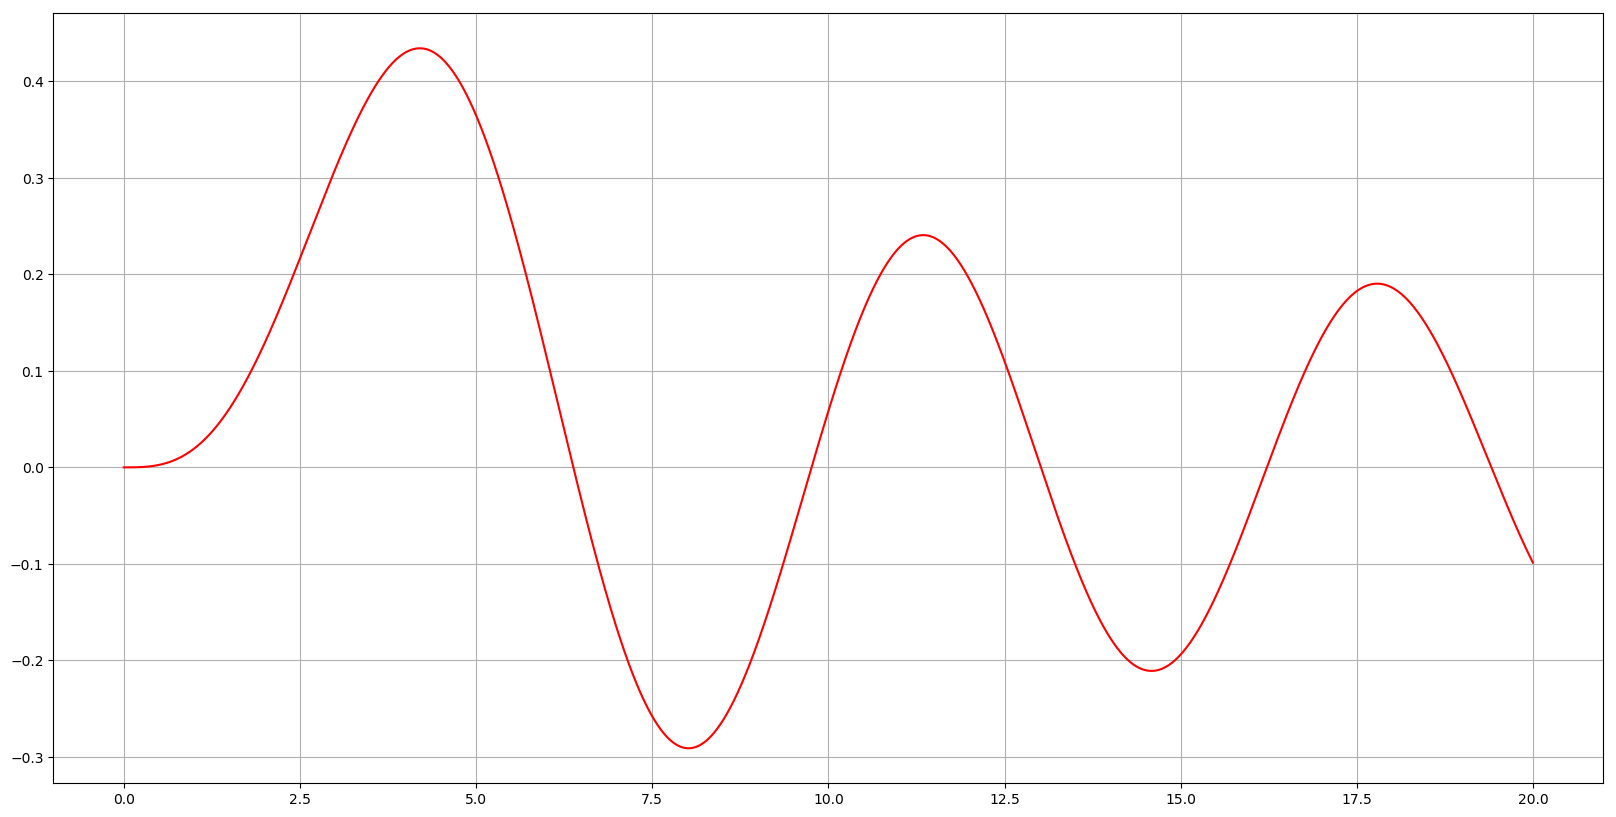
\includegraphics[width=\textwidth]{{../img/23-j3}.png}
	\caption{$J_3(x)$}
\end{figure}
\begin{figure}[H]
	\centering
	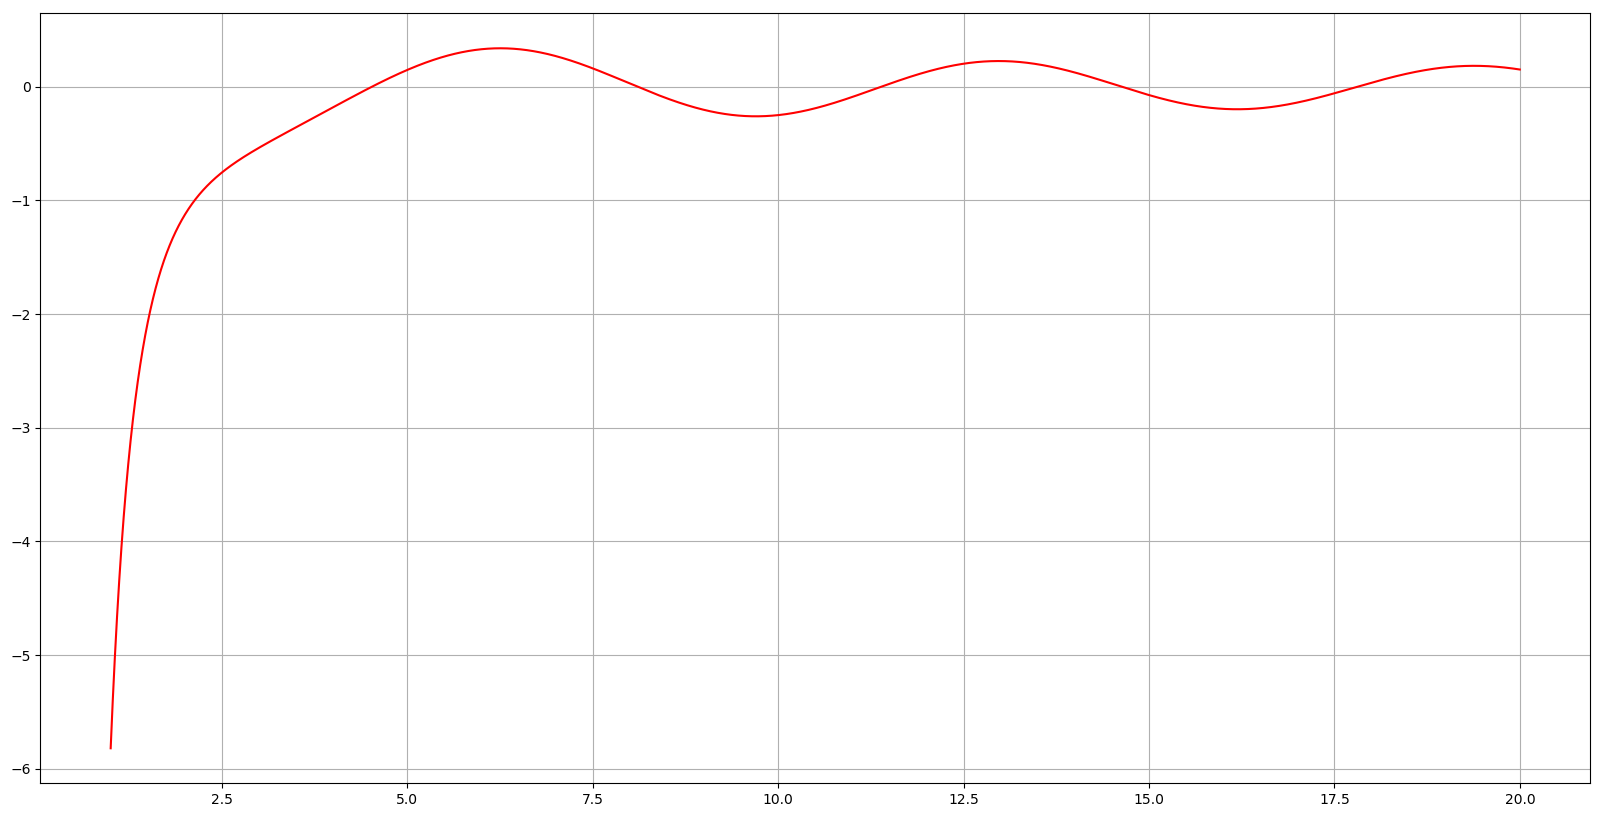
\includegraphics[width=\textwidth]{{../img/23-n3}.png}
	\caption{$N_3(x)$}
\end{figure}
 
Другий клас функцій Бесселя --- функції Бесселя уявного аргументу можна отримати як два лінійно–незалежних розв'язки рівняння \eqref{eq:4.7.2}, зокрема їх можна записати за формулою \eqref{eq:4.7.10} з використанням заміни змінної $x := i x$ в результаті будемо мати функцію Бесселя першого роду уявного аргументу:
\begin{equation}
	\label{eq:4.7.17}
	I_\nu(x) = \frac{J_\nu(i x)}{i^\nu} = \Sum_{k = 0}^\infty \frac{(x/2)^{2 k + \nu}}{k! \cdot \Gamma(k + \nu + 1)}, \quad 0 < x < \infty.
\end{equation}

Другий лінійно-незалежний розв'язок для нецілих $\nu$ можна отримати аналогічно попередньому розв'язку з формули \eqref{eq:4.7.10'}:
\begin{equation}
	\label{eq:4.7.18}
	I_{-\nu}(x) = i^\nu J_{-\nu}(i x) = \Sum_{k = 0}^\infty \frac{(x/2)^{2 k - \nu}}{k! \cdot \Gamma(k - \nu + 1)}, \quad 0 < x < \infty.
\end{equation}

Легко бачити, що при $\nu = n$ функції $I_n(x) = I_{-n}(x)$, тобто є лінійно залежними між собою і не можуть бути використані для запису загального розв'язку рівняння \eqref{eq:4.7.2}. \medskip

Функцію другого роду уявного аргументу будують у вигляді лінійної комбінації
\begin{equation}
	\label{eq:4.7.19}
	K_\nu(x) = \frac{\pi (I_{-\nu}(x) - I_\nu(x))}{2 \sin (\nu \pi)}.
\end{equation}

Враховуючи, що $I_n(x) = I_{-n}(x)$, остання формула має невизначеність типу $0/0$ при $\nu = n$. Розкриваючи її за правилом Лопіталя отримаємо 
\begin{equation}
	\label{eq:4.7.20}
	K_n(x) = \frac{(-1)^n}{2} \left( \left( \frac{\partial I_{-\nu}(x)}{\partial \nu} \right)_{\nu = n} - \left( \frac{\partial I_\nu(x)}{\partial \nu} \right)_{\nu = n} \right).
\end{equation}

\begin{definition}
	Функцію $K_\nu(x)$ називають функцією другого роду уявного аргументу, або функцією Макдональда вона має наступний вигляд:
	\begin{equation}
		\label{eq:4.7.21}
		\begin{aligned}
			K_n(x) &= -I_n(x) \ln \frac{x}{2} + \frac{1}{2} \Sum_{k = 0}^\infty \frac{(x/2)^{n + 2 k}}{k! (n - k)!} \left( \Psi(k + 1) + \Psi(k + n + 1) \right) + \\
			& \quad + \frac{1}{2} \Sum_{k=0}^{n-1} \frac{(-1)^k (n - k - 1)!}{k!} \left(\frac{2}{x}\right)^{n-2k}.
		\end{aligned}
	\end{equation}
\end{definition}

Виходячи з рекурентних співвідношень \eqref{eq:4.7.14}, \eqref{eq:4.7.14'}, можна отримати рекурентні співвідношення для функцій Бесселя уявного аргументу першого та другого роду:
\begin{gather}
	\label{eq:4.7.22}
	\frac{\diff}{\diff x} I_\nu(x) - \frac{\nu}{x} \cdot I_\nu(x) = I_{\nu+1}(x) \qquad \frac{\diff}{\diff x} I_\nu(x) + \frac{\nu}{x} \cdot I_\nu(x) = I_{\nu-1}(x), \\
	\label{eq:4.7.23}
	\frac{\diff}{\diff x} K_\nu(x) + \frac{\nu}{x} \cdot K_\nu(x) = -K_{\nu-1}(x) \qquad \frac{\diff}{\diff x} K_\nu(x) + \frac{\nu}{x} \cdot K_\nu(x) = -K_{\nu+1}(x).
\end{gather}

Відмітимо також характер поведінки функцій Бесселя уявного аргументу при $x = 0$ та $x \to \infty$. \medskip

Виходячи з формул \eqref{eq:4.7.17} та \eqref{eq:4.7.21} можна зробити висновок, що
\begin{gather}
	\label{eq:4.7.24}
	I_\nu(x) = O(x^\nu), \quad x \to 0, \\
	\label{eq:4.7.25}
	K_\nu(x) = O(x^{-\nu}), \quad \nu > 0, \qquad K_0(x) = O(\ln(x)), \quad x \to 0, \\
	\label{eq:4.7.26}
	I_\nu(x) \approx \sqrt{\frac{1}{2 \pi x}} \cdot e^x, \qquad K_\nu(x) \approx \sqrt{\frac{\pi}{2 x}} \cdot e^{-x}, \quad x \to \infty.
\end{gather}

Наведемо графіки функцій $I_3(x)$ та $K_3(x)$:
\begin{figure}[H]
	\centering
	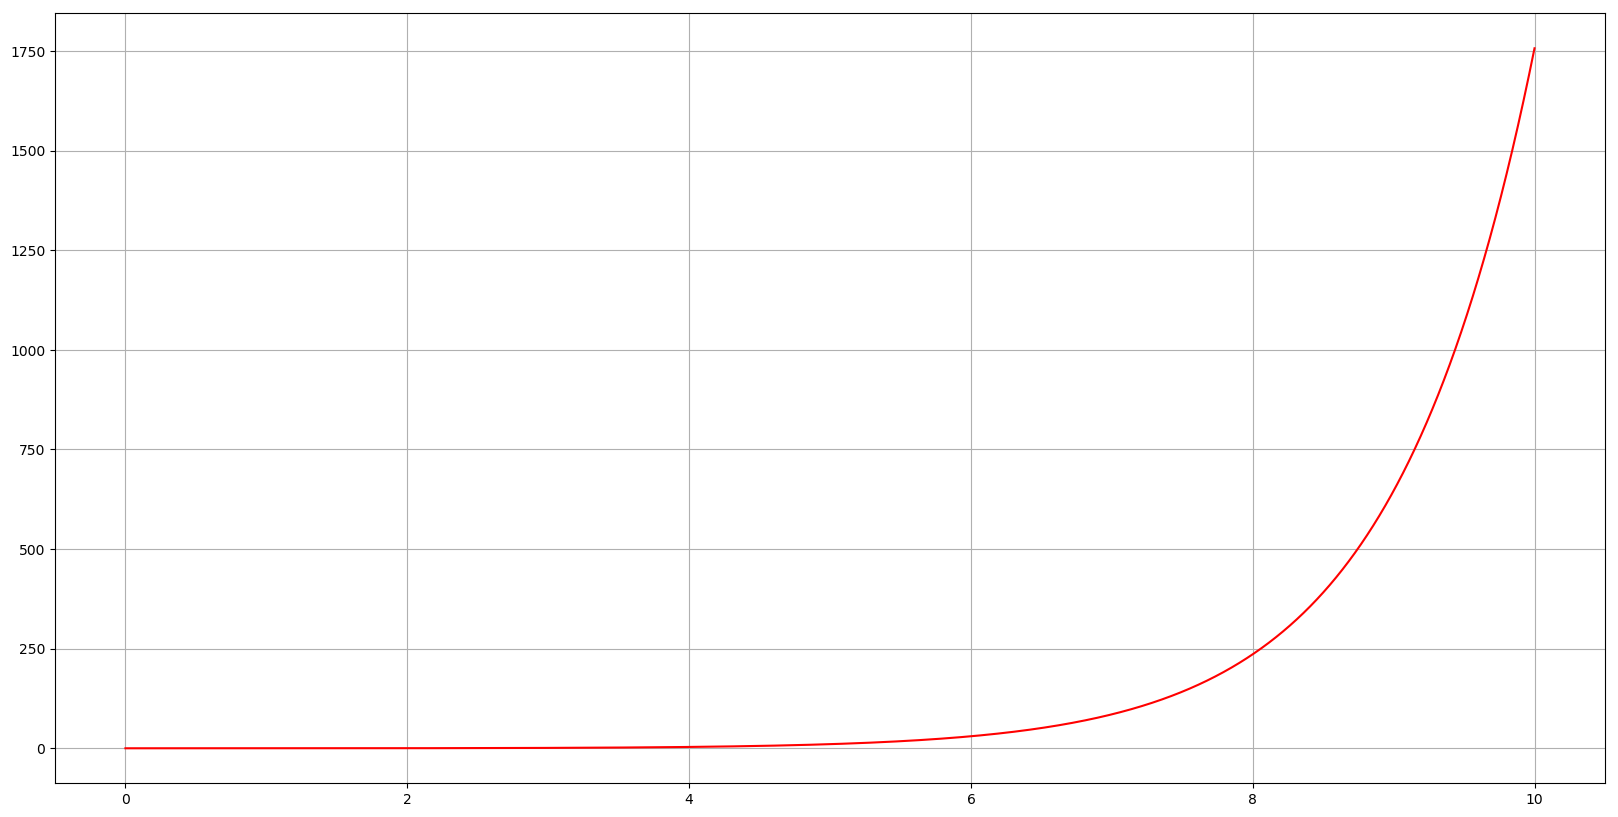
\includegraphics[width=\textwidth]{{../img/23-i3}.png}
	\caption{$I_3(x)$}
\end{figure}
\begin{figure}[H]
	\centering
	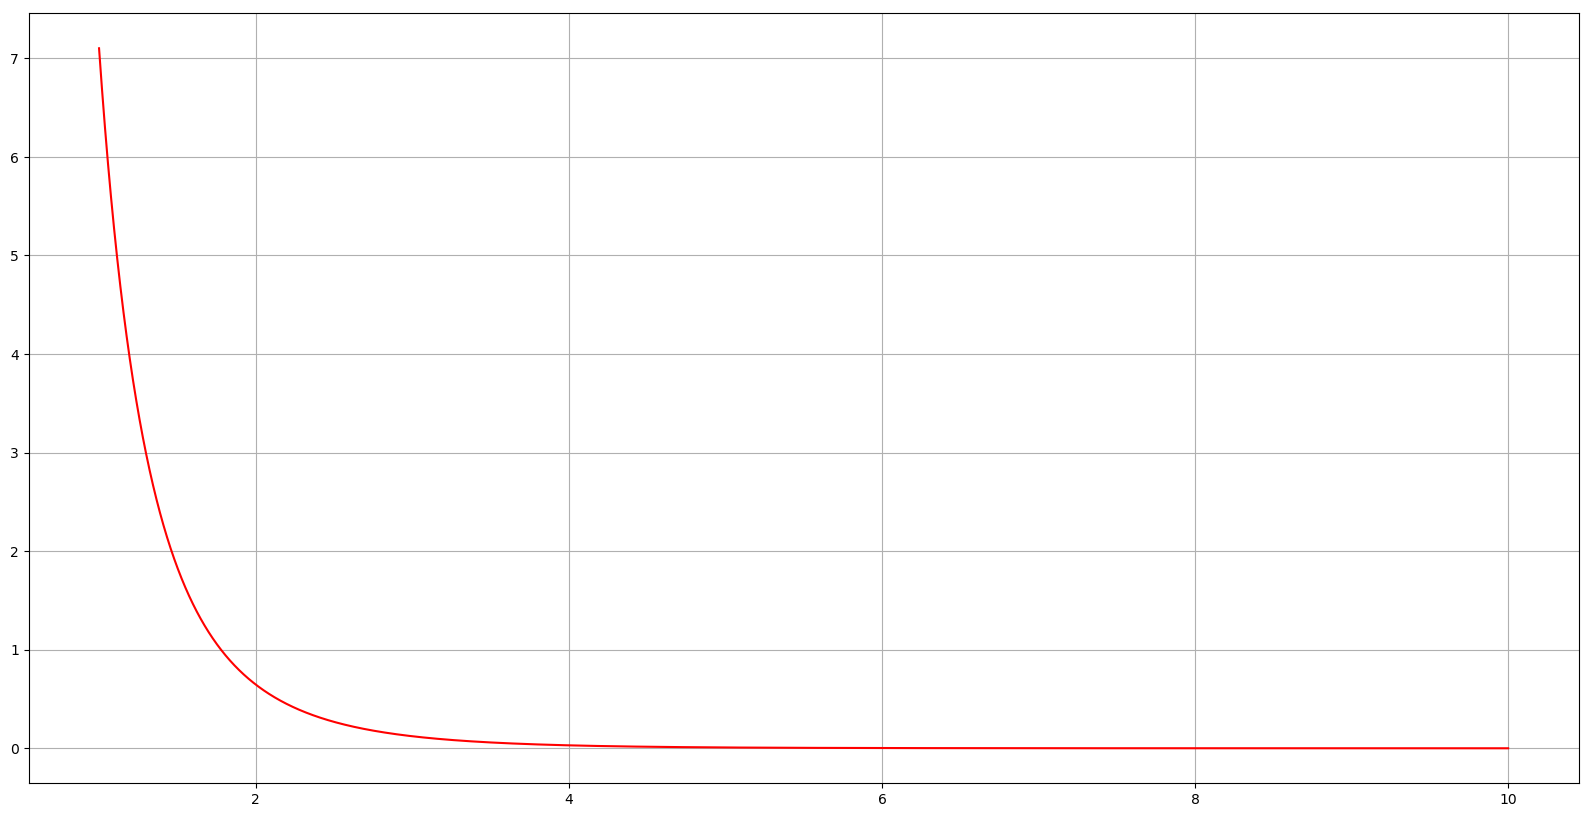
\includegraphics[width=\textwidth]{{../img/23-k3}.png}
	\caption{$K_3(x)$}
\end{figure}

\end{document}
	\end{figure}
	для кожного $\omega_i$, $i = \overline{1..p}$ знайдемо множину
	\begin{equation}
	    \text{First}_1(\omega_i) \oplus_1 \text{Follow}_1(A) = L_i = \left\{a_i^1, a_i^2, \ldots, a_i^{n_i}\right\}.
	\end{equation}

	Оскільки за умовою $L_i \cap L_j = \varnothing$, $i \ne j$, то відповідний фрагмент програми на мові С матиме вигляд:
	\begin{verbatim}
	extern int lexem_code;
	extern char lexem_text[];
	...
	void f_A_i(void) {
	    switch(lexema_code) {
	        case code_a_1_1:
	        case code_a_1_2:
	        ...
	        case code_a_1_n_1:
	            ...  // фрагмент програми для w_1
	            break;
	        case code_a_2_1:
	        case code_a_2_2:
	        ...
	        case code_a_2_n_2:
	            ...  // фрагмент програми для w_2
	            break;
	        ...
	        ...
	        ...
	        case code_a_p_1:
	        case code_a_p_2:
	        ...
	        case code_a_p_n_p:
	            ...  // фрагмент програми для w_p
	            break;
	        default: 
	            error();
	    }
	}  // кінець функції для нетермінала A_i
	\end{verbatim}
\end{itemize}

Відмітимо, що до того, як зменшувати кількість синтаксичних діаграм шляхом суперпозиції одних діаграм в інші, необхідно знайти контексти виду $\text{First}_1(\omega_i) \oplus_1 \text{Follow}_1(A)$ для тієї синтаксичної діаграми нетермінала $A$, для якої ми виконуємо операцію суперпозиції. Ці контексти ми використаємо при програмуванні синтаксичного аналізатора на основі синтаксичної діаграми, у яку підставлено синтаксичну діаграму для нетермінала $A_i$.

\subsubsection{Одна особливість}

Досить часто при визначенні синтаксису мови програмування користуються синтаксичними правилами виду $A_i \mapsto \alpha_1 \alpha_2 \ldots \alpha_p A_i \mid \varepsilon$. Тоді синтаксична діаграма буде мати вигляд:
\begin{figure}[H]
	\centering
	% cd ..\..\Users\NikitaSkybytskyi\Desktop\c3s1\complex-analysis
\documentclass[a4paper, 12pt]{article}
\usepackage[utf8]{inputenc}
\usepackage[english, ukrainian]{babel}

\usepackage{amsmath, amssymb}
\usepackage{multicol}
\usepackage{graphicx}
\usepackage{float}
\usepackage{multicol}

\usepackage{amsthm}
\newtheorem{theorem}{Теорема}[subsection]
\newtheorem*{theorem*}{Теорема}
\newtheorem{lemma}{Лема}[subsection]
\newtheorem*{lemma*}{Лема}
\newtheorem*{remark*}{Зауваження}
\theoremstyle{definition}
\newtheorem*{definition}{Визначення}
\newtheorem{problem}{Задача}[section]
\newtheorem*{solution}{Розв'язок}
\newtheorem{example}{Приклад}
\newtheorem*{example*}{Приклад}
\newtheorem*{hint}{Вказівка}

\newcommand{\Max}{\displaystyle\max\limits}
\newcommand{\Sum}{\displaystyle\sum\limits}
\newcommand{\Int}{\displaystyle\int\limits}
\newcommand{\Lim}{\displaystyle\lim\limits}

\newcommand{\RR}{\mathbb{R}}
\newcommand{\ZZ}{\mathbb{Z}}

\newcommand*\diff{\mathop{}\!\mathrm{d}}
\newcommand*\Diff[1]{\mathop{}\!\mathrm{d^#1}}

\DeclareMathOperator{\Real}{Re}
\DeclareMathOperator{\Imag}{Im}

\DeclareMathOperator{\Arg}{Arg}

\DeclareMathOperator{\Ln}{Ln}

\DeclareMathOperator{\Arctan}{Arctan}
\DeclareMathOperator{\Arcsin}{Arcsin}
\DeclareMathOperator{\Arccos}{Arccos}
\DeclareMathOperator{\Arccosh}{Arccosh}
\DeclareMathOperator{\Arctanh}{Arctanh}

\DeclareMathOperator{\arcsinh}{arcsinh}
\DeclareMathOperator{\arccosh}{arccosh}
\DeclareMathOperator{\arctanh}{arctanh}
\DeclareMathOperator{\arccoth}{arccoth}

\newcommand{\varLimsup}{\varlimsup\limits}

\makeatletter
\newcommand\xLeftrightarrow[2][]{%
  \ext@arrow 9999{\longLeftrightarrowfill@}{#1}{#2}}
\newcommand\longLeftrightarrowfill@{%
  \arrowfill@\Leftarrow\relbar\Rightarrow}
\makeatother

\renewcommand{\epsilon}{\varepsilon}
\renewcommand{\phi}{\varphi}

\allowdisplaybreaks
\setlength\parindent{0pt}
\numberwithin{equation}{subsection}

\usepackage{xcolor}
\usepackage{hyperref}
\hypersetup{unicode=true,colorlinks=true,linktoc=all,linkcolor=red}

\numberwithin{equation}{section}% reset equation counter for sections
\numberwithin{equation}{subsection}
% Omit `.0` in equation numbers for non-existent subsections.
\renewcommand*{\theequation}{%
  \ifnum\value{subsection}=0 %
    \thesection
  \else
    \thesubsection
  \fi
  .\arabic{equation}%
}


\title{{\Huge МАТЕМАТИЧНА ФІЗИКА}}
\author{Скибицький Нікіта}
\date{\today}
 
\usepackage{amsthm}
\usepackage[dvipsnames]{xcolor}
\usepackage{thmtools}
\usepackage[framemethod=TikZ]{mdframed}

\theoremstyle{definition}
\mdfdefinestyle{mdbluebox}{%
	roundcorner = 10pt,
	linewidth=1pt,
	skipabove=12pt,
	innerbottommargin=9pt,
	skipbelow=2pt,
	nobreak=true,
	linecolor=blue,
	backgroundcolor=TealBlue!5,
}
\declaretheoremstyle[
	headfont=\sffamily\bfseries\color{MidnightBlue},
	mdframed={style=mdbluebox},
	headpunct={\\[3pt]},
	postheadspace={0pt}
]{thmbluebox}

\mdfdefinestyle{mdredbox}{%
	linewidth=0.5pt,
	skipabove=12pt,
	frametitleaboveskip=5pt,
	frametitlebelowskip=0pt,
	skipbelow=2pt,
	frametitlefont=\bfseries,
	innertopmargin=4pt,
	innerbottommargin=8pt,
	nobreak=true,
	linecolor=RawSienna,
	backgroundcolor=Salmon!5,
}
\declaretheoremstyle[
	headfont=\bfseries\color{RawSienna},
	mdframed={style=mdredbox},
	headpunct={\\[3pt]},
	postheadspace={0pt},
]{thmredbox}

\declaretheorem[%
style=thmbluebox,name=Теорема,numberwithin=section]{theorem}
\declaretheorem[style=thmbluebox,name=Лема,sibling=theorem]{lemma}
\declaretheorem[style=thmbluebox,name=Твердження,sibling=theorem]{proposition}
\declaretheorem[style=thmbluebox,name=Наслідок,sibling=theorem]{corollary}
\declaretheorem[style=thmredbox,name=Приклад,sibling=theorem]{example}

\mdfdefinestyle{mdgreenbox}{%
	skipabove=8pt,
	linewidth=2pt,
	rightline=false,
	leftline=true,
	topline=false,
	bottomline=false,
	linecolor=ForestGreen,
	backgroundcolor=ForestGreen!5,
}
\declaretheoremstyle[
	headfont=\bfseries\sffamily\color{ForestGreen!70!black},
	bodyfont=\normalfont,
	spaceabove=2pt,
	spacebelow=1pt,
	mdframed={style=mdgreenbox},
	headpunct={ --- },
]{thmgreenbox}

\mdfdefinestyle{mdblackbox}{%
	skipabove=8pt,
	linewidth=3pt,
	rightline=false,
	leftline=true,
	topline=false,
	bottomline=false,
	linecolor=black,
	backgroundcolor=RedViolet!5!gray!5,
}
\declaretheoremstyle[
	headfont=\bfseries,
	bodyfont=\normalfont\small,
	spaceabove=0pt,
	spacebelow=0pt,
	mdframed={style=mdblackbox}
]{thmblackbox}

% \theoremstyle{theorem}
\declaretheorem[name=Запитання,sibling=theorem,style=thmblackbox]{ques}
\declaretheorem[name=Вправа,sibling=theorem,style=thmblackbox]{exercise}
\declaretheorem[name=Зауваження,sibling=theorem,style=thmgreenbox]{remark}

\theoremstyle{definition}
\newtheorem{claim}[theorem]{Твердження}
\newtheorem{definition}[theorem]{Визначення}
\newtheorem{fact}[theorem]{Факт}

\newtheorem{problem}{Задача}[section]
\renewcommand{\theproblem}{\thesection\Alph{problem}}
\newtheorem{sproblem}[problem]{Задача}
\newtheorem{dproblem}[problem]{Задача}
\renewcommand{\thesproblem}{\theproblem$^{\star}$}
\renewcommand{\thedproblem}{\theproblem$^{\dagger}$}
\newcommand{\listhack}{$\empty$\vspace{-2em}} 

\begin{document}

\tableofcontents

\setcounter{section}{4}
\setcounter{subsection}{7}

\subsection{Потенціали операторів Лапласа та Гельмгольца, їх властивості}

Теорія потенціалів є дуже ефективним засобом дослідження існування і єдності розв'язків граничних задач для еліптичних та параболічних рівнянь. За допомогою потенціалів граничні задачі можна звести до інтегральних рівнянь Фредгольма другого роду з полярним ядром, а іноді до інтегральних рівнянь Фредгольма першого роду з сингулярним або навіть гіперсингулярним ядром. \medskip

При отримані замість граничної задачі інтегрального рівняння Фредгольма дослідження існування і єдності розв'язку можна проводити використовуючи теорію Фредгольма для інтегральних рівнянь. \medskip

Крім того, використовуючи потенціали можна побудувати більш ефективні чисельні методи знаходження розв'язків граничних задач.

\begin{definition}
	Чисельні методи які базуються на теорії потенціалу називають \textit{методами граничних інтегральних рівнянь}.
\end{definition}

Введемо потенціали для основних еліптичних операторів Лапласа і Гельмгольца для тривимірного евклідового простору: 
\begin{longtable}{p{.5\textwidth} p{.5\textwidth}}
	\parbox{.5\textwidth}{\begin{equation}
		\label{eq:4.8.1}
		U(x) = \Iiint_\Omega \frac{\rho(y)}{4 \pi |x - y|} \diff y
	\end{equation}} & \parbox{.5\textwidth}{\begin{equation}
		\label{eq:4.8.1'}
		U^k(x) = \Iiint_\Omega \frac{e^{\pm i k |x - y|} \rho(y)}{4 \pi |x - y|} \diff y
	\end{equation}} \\
	\parbox{.5\textwidth}{\begin{equation}
		\label{eq:4.8.2}
		V(x) = \Iint_S \frac{\mu(y)}{4 \pi |x - y|} \diff S_y
	\end{equation}} & \parbox{.5\textwidth}{\begin{equation}
		\label{eq:4.8.2'}
		V^k(x) = \Iint_S \frac{e^{\pm i k |x - y|} \mu(y)}{4 \pi |x - y|} \diff S_y
	\end{equation}} \\
	\parbox{.5\textwidth}{\begin{equation}
		\label{eq:4.8.3}
		W(x) = \Iint_S \sigma(y) \frac{\partial}{\partial \vec n_y} \frac{1}{4 \pi |x - y|} \diff S_y
	\end{equation}} & \parbox{.5\textwidth}{\begin{equation}
		\label{eq:4.8.3'}
		W^k(x) = \Iint_S \sigma(y) \frac{\partial}{\partial \vec n_y} \frac{e^{\pm i k |x - y|}}{4 \pi |x - y|} \diff S_y
	\end{equation}}
\end{longtable}

\begin{definition}
	Інтеграли \eqref{eq:4.8.1}, \eqref{eq:4.8.1'} будемо називати \textit{потенціалом об'єму} для операторів Лапласа та Гельмгольца відповідно. Інтеграли \eqref{eq:4.8.2}, \eqref{eq:4.8.2'} будемо називати \textit{потенціалами простого шару} (слоя) для операторів Лапласа та Гельмгольца відповідно. Інтеграли \eqref{eq:4.8.3}, \eqref{eq:4.8.3'} будемо називати \textit{потенціалами подвійного шару} (слоя) для операторів Лапласа та Гельмгольца відповідно.
\end{definition}

\begin{definition}
	При цьому функції $\rho, \mu, \sigma$ називають \textit{щільностями потенціалів}, які задані в області $\Omega$ або на поверхні $S$.
\end{definition}

Як легко бачити, при записі усіх потенціалів використовується фундаментальний розв'язок відповідного оператора: фундаментальний розв'язок оператора Лапласа
\begin{equation}
	\frac{1}{4 \pi |x - y|}
\end{equation}
для потенціалів об'єму, простого шару і подвійного шару для оператора Лапласа, або фундаментальний розв'язок оператора Гельмгольца
\begin{equation}
	\frac{e^{\pm i k |x - y|}}{4 \pi |x - y|}	
\end{equation}
для потенціалів об'єму, простого шару і подвійного шару. \medskip

Аналогічно потенціалам для операторів Лапласа і Гельмгольца в тривимірному просторі можна ввести потенціали і для двовимірного простору. При цьому треба використовувати фундаментальні розв'язки оператора Лапласа і Гельмгольца в двовимірному просторі. \medskip

Нагадаємо, що фундаментальний розв'язок рівняння Лапласа при $n = 2$ має вигляд
\begin{equation}
	q_0(|x - y|) = \frac{1}{2 \pi} \ln \frac{1}{|x - y|},
\end{equation}
а фундаментальний розв'язок для оператора Гельмгольца при $n = 2$ можна записати у вигляді 
\begin{equation}
	\label{eq:4.8.4}
	q_k (|x - y|) = \pm \frac{i}{4} \left( J_0(k |x - y|) \pm i N(k |x - y|) \right),
\end{equation}
де функції $J_0(x), N_0(x)$ --- функції Бесселя нульового порядку першого і другого роду.  \medskip

Відповідно до вигляду фундаментальних розв'язків, потенціали в двовимірному просторі матимуть вигляд:
\begin{longtable}{p{.5\textwidth} p{.5\textwidth}}
	\parbox{.5\textwidth}{\begin{equation}
		\label{eq:4.8.5}
		U_0(x) = \Iint_D \rho(y) q_0(|x - y|) \diff y
	\end{equation}} & \parbox{.5\textwidth}{\begin{equation}
		\label{eq:4.8.5'}
		U_k(x) = \Iint_D \rho(y) q_k(|x - y|) \diff y
	\end{equation}} \\
	\parbox{.5\textwidth}{\begin{equation}
		\label{eq:4.8.6}
		V_0(x) = \Oint_C \mu(y) q_0(|x - y|) \diff \ell_y
	\end{equation}} & \parbox{.5\textwidth}{\begin{equation}
		\label{eq:4.8.6'}
		V_k(x) = \Oint_C \mu(y) q_k(|x - y|) \diff \ell_y
	\end{equation}} \\
	\parbox{.5\textwidth}{\begin{equation}
		\label{eq:4.8.7}
		W_0(x) = \Oint_C \sigma(y) \frac{\partial q_0(|x - y|)}{\partial \vec n_y} \diff \ell_y
	\end{equation}} & \parbox{.5\textwidth}{\begin{equation}
		\label{eq:4.8.7'}
		W_k(x) = \Oint_C \sigma(y) \frac{\partial q_k(|x - y|)}{\partial \vec n_y} \diff \ell_y
	\end{equation}}
\end{longtable}

Відмітимо, що властивості потенціалів залежать від декількох факторів, перелічимо їх:
\begin{itemize}
	\item властивостей щільностей потенціалів;
	\item положення точки $x$ (належить $x$ області інтеграції або не належить);
	\item властивості поверхні $S$ для потенціалів простого і подвійного шару.
\end{itemize}

\subsubsection{Властивості потенціалів поза областю інтеграції}

\begin{theorem}[про властивості потенціалів поза областю інтеграції]
	\label{th:4.8.1}
	Якщо щільності потенціалів простого і подвійного шару інтегровані на поверхні $S$, ($\iint_S |\mu(y)| \diff S_y < \infty$, $\iint_S |\sigma(y)| \diff S_y < \infty$), а потенціал об'єму --- інтегрована в області $\Omega$, )$\iiint_\Omega |\rho(y)| \diff y < \infty$), то відповідні потенціали для оператору Лапласа і Гельмгольца є функціями які мають неперервні похідні будь-якого порядку в довільній області $\Omega_1$, яка не перетинається з областю інтегрування ($\Omega$ для потенціалу об'єму та $S$ для потенціалів простого та подвійного шару) і в кожній точці $\Omega_1$ ці потенціали задовольняють рівняння Лапласа або Гельмгольца відповідно.
\end{theorem}

Доведення теореми для будь-якого з потенціалів практично не відрізняється, тому продемонструємо доведення для випадку потенціалу простого шару оператора Гельмгольца. 

\begin{proof}
	Оскільки щільність потенціалу простого шару $\mu$ інтегрована на $S$, а функція
	\begin{equation}
		\frac{e^{\pm i k |x - y|}}{4 \pi |x - y|}
	\end{equation}
	є неперервно-диференційованою скільки завгодно разів у випадку, коли $(x, y) \in (\Omega_1, S)$, $\Omega_1 \cap S = \emptyset$, то можна застосувати теорему про можливість диференціювання такого інтегралу, шляхом обчислення похідної від підінтегральної функції. \medskip

	Тобто
	\begin{equation}
		D^\alpha V^k(x) = \Iint_S \mu(y) D^\alpha \left( \frac{e^{\pm i k |x - y|}}{4 \pi |x - y|} \right) \diff S_y, \quad x \in \Omega_1,
	\end{equation}
	оскільки підінтегральна функція є неперервною функцією аргументу $x$, майже для кожного $y \in S$, то 
	\begin{equation}
		\Iint_S \mu(y) D^\alpha \left( \frac{e^{\pm i k |x - y|}}{4 \pi |x - y|} \right) \diff S_y \in C(\Omega_1).
	\end{equation}

	Оскільки потенціал має неперервні похідні будь-якого порядку, то
	\begin{equation}
		(\Delta + k^2) V^k(x) = \Iint_S \mu(y) (\Delta_x + k^2) \left( \frac{e^{\pm i k |x - y|}}{4 \pi |x - y|} \right) \diff S_y = 0, \quad x \in \Omega_1.
	\end{equation}

	Останній інтеграл дорівнює нулю, оскільки при $x \ne y$:
	\begin{equation}
		(\Delta_x + k^2) \left( \frac{e^{\pm i k |x - y|}}{4 \pi |x - y|} \right) \equiv 0.
	\end{equation}
\end{proof}

\begin{theorem}[про неперервність і неперервну диференційованість потенціалу об'єму]
	\label{th:4.8.2}
	Якщо щільність потенціалу об'єму інтегрована в області $\Omega$, то потенціал об'єму для оператора Лапласа і Гельмгольца \eqref{eq:4.8.1} та \eqref{eq:4.8.1'} є неперервними і неперервно-диференційованими функціями в усьому евклідовому просторі $\RR^3$.
\end{theorem}

\begin{proof}
	Розглянемо функцію
	\begin{equation}
		\rho_1(y) = \begin{cases}
			\rho(y), & y \in \Omega, \\
			0, & y \in \Omega'.
		\end{cases}	
	\end{equation}

	Функція $\rho_1$ залишається інтегрованою в будь-якій області $\Omega_1 \in \RR^3$. \medskip

	Нехай $x \in \RR^3$ --- довільна точка. Розглянемо будь-яку область, яка містить точку $x$, нехай це область $\Omega_1$, тоді
	\begin{equation}
		U^k(x) = \Iiint_{\Omega_1} \frac{e^{\pm i k |x - y|}}{4 \pi |x - y|} \rho_1(y) \diff y.
	\end{equation}

	На останню формулу будемо дивитися як на результат відображення деякої функції $\rho_1 \in L_2(\Omega_1)$ за допомогою полярного ядра
	\begin{equation}
		K(x, y) = \frac{e^{\pm i k |x - y|}}{4 \pi |x - y|}.
	\end{equation}

	Відомо, що результатом відображення буде функція $U_k \in C(\Omega_1)$.  Таким чином неперервність потенціалу доведена. \medskip

	Розглянемо тепер функцію
	\begin{equation}
		U_k^{(s)}(x) = \Iiint_{\Omega_1} \frac{\partial}{\partial x_s} \frac{e^{\pm i k |x - y|}}{4 \pi |x - y|} \rho_1(y) \diff y.
	\end{equation}

	Для неї:
	\begin{equation}
		\begin{aligned}
			\frac{\partial}{\partial x_s} \frac{e^{\pm i k |x - y|}}{4 \pi |x - y|} &= \frac{(\pm i k |x - y| - 1) e^{\pm i k |x - y|}}{4 \pi |x - y|^2} \frac{\partial |x - y|}{\partial x_s} = \\
			&= \frac{(\pm i k |x - y| - 1) e^{\pm i k |x - y|}}{4 \pi |x - y|^2} \frac{x_s - y_s}{|x - y|} = \frac{A_s(x, y)}{|x - y|^2},
		\end{aligned}
	\end{equation} 
	де $A_s$ --- неперервна функція. Таким чином
	\begin{equation}
		\frac{\partial}{\partial x_s} \frac{e^{\pm i k |x - y|}}{4 \pi |x - y|}	
	\end{equation}
	є полярним ядром в будь-який області тривимірного простору. \medskip

	А це означає що
	\begin{equation}
		U_k^{(s)}(x) = \Iiint_{\Omega_1} \frac{\partial}{\partial x_s} \frac{e^{\pm i k |x - y|}}{4 \pi |x - y|} \rho_1(y) \diff y,
	\end{equation}
	як результат відображення функції $\rho_1 \in L_2(\Omega_2)$ за допомогою полярного ядра є неперервною функцією. Тобто $U_k^{(s)} \in C(\Omega_2)$. \medskip

	Покажемо тепер, що
	\begin{equation}
		U_k^{(s)}(x) = \frac{\partial U_k(x)}{\partial x_s}.
	\end{equation}

	Розглянемо
	\begin{equation}
		\begin{aligned}
			\Int_{z_0}^{z_s} U_k^{(s)}(\ldots, x_s, \ldots) \diff x_s &= \Int_{z_0}^{z_s} \Iiint_{\Omega_1} \frac{\partial}{\partial x_s} \frac{e^{\pm i k |x - y|}}{4 \pi |x - y|} \rho_1(y) \diff y \diff x_s = \\
			&= \Iiint_{\Omega_1} \rho_1(y) \Int_{z_0}^{z_s} \frac{\partial}{\partial x_s} \frac{e^{\pm i k |x - y|}}{4 \pi |x - y|} \rho_1(y) \diff x_s \diff y = \\
			&= \left. \Iiint_{\Omega_1} \frac{e^{\pm i k |x - y|}}{4 \pi |x - y|} \rho_1(y) \diff y \right|_{x_s = z_s} - \\
			& \quad - \left. \Iiint_{\Omega_1} \frac{e^{\pm i k |x - y|}}{4 \pi |x - y|} \rho_1(y) \diff y \right|_{x_s = z_0} = \\
			&= \left. U_k(x) \right|_{x_s = z_s} - \left. U_k(x) \right|_{x_s = z_0}.
		\end{aligned}
	\end{equation}
	Вважаємо точку $z_s$ змінною, а $z_0$ фіксованою і обчислимо похідну від лівої і правої частини останньої рівності:
	\begin{equation}
		\frac{\partial U_k(\ldots, z_s, \ldots)}{\partial z_s} = U_k^{(s)} (\ldots, z_s, \ldots).
	\end{equation}
\end{proof}

\begin{theorem}[про другі похідні потенціалу об'єму]
	\label{th:4.8.3}
	Якщо цільність потенціалу об'єму $\rho \in C^{(1)}(\Omega) \cap C(\overline{\Omega})$, то об'ємний потенціал \eqref{eq:4.8.1} і \eqref{eq:4.8.1'} має в області $\Omega$ неперервні похідні другого порядку і задовольняє відповідно рівнянню Пуассона:
	\begin{equation}
		\label{eq:4.8.8}
		\Delta U(x) = - \rho(x), \quad x \in \Omega,
	\end{equation}
	або неоднорідному рівнянню Гельмгольца 
	\begin{equation}
		\label{eq:4.8.8'}
		(\Delta + k^2) U_k(x) = - \rho(x), \quad x \in \Omega.
	\end{equation}
\end{theorem}

Доведення проведемо для потенціалу об'єму оператора Гельмгольца в тривимірному випадку. Усі інші випадки розглядаються аналогічно.

\begin{proof}
	Оскільки щільність потенціалу є неперервною, то згідно до теореми \ref{th:4.8.2} потенціал об'єму має неперервні перші похідні зокрема і в області $\Omega$. Обчислимо похідну потенціалу об'єму:
	\begin{equation}
		\label{eq:4.8.9}
		\begin{aligned}
			\frac{\partial U_k(x)}{\partial x_j} &= \Iiint_\Omega \rho(y) \frac{\partial}{\partial x_j} \frac{e^{\pm i k |x - y|}}{4 \pi |x - y|} \diff y = - \Iiint_\Omega \rho(y) \frac{\partial}{\partial y_j} \frac{e^{\pm i k |x - y|}}{4 \pi |x - y|} \diff y = \\
			&= \Iiint_\Omega \frac{\partial \rho(y)}{\partial y_j} \frac{e^{\pm i k |x - y|}}{4 \pi |x - y|} \diff y - \Iint_S \rho(y) \frac{e^{\pm i k |x - y|}}{4 \pi |x - y|} \cos(\vec n, y_j) \diff S_y
		\end{aligned}
	\end{equation}

	Тут була використана формула інтегрування за частинами. Таким чином перша частинна похідна потенціалу об'єму представлена у вигляді двох потенціалів: потенціалу об'єму з неперервною щільністю $\partial \rho / \partial y_j$ і потенціалу простого шару з щільністю $\rho(y) \cos(\vec n, y_j)$. З теореми \ref{th:4.8.2} випливає що перший доданок --- потенціал об'єму --- є неперервно-диференційована функція, а з теореми \ref{th:4.8.1} випливає, що другий доданок --- потенціал простого шару --- теж є неперервно-диференційована функція. \medskip

	Таким чином можна обчислити другу похідну, шляхом диференціювання рівності \eqref{eq:4.8.9}:
	\begin{equation}
		\begin{aligned}
			\frac{\partial^2 U_k(x)}{\partial x_j^2} &= \Iiint_\Omega \frac{\partial \rho(y)}{\partial y_j} \frac{\partial}{\partial x_j} \frac{e^{\pm i k |x - y|}}{4 \pi |x - y|} \diff y - \\
			& \quad - \Iint_S \rho(y) \frac{\partial}{\partial x_j} \frac{e^{\pm i k |x - y|}}{4 \pi |x - y|} \cos(\vec n_y, y_j) \diff S_y = \\
			&= \Iiint_\Omega \frac{\partial \rho(y)}{\partial y_j} \frac{\partial}{\partial y_j} \frac{e^{\pm i k |x - y|}}{4 \pi |x - y|} \diff y - \\
			& \quad - \Iint_S \rho(y) \frac{\partial}{\partial y_j} \frac{e^{\pm i k |x - y|}}{4 \pi |x - y|} \cos(\vec n_y, y_j) \diff S_y = A.
		\end{aligned}
	\end{equation}

	Перший доданок в правій частині останньої рівності є невласним інтегралом, запишемо його у вигляді:
	\begin{equation}
		\begin{aligned}
			A &= \Lim_{\epsilon \to 0} \Iiint_{\Omega \setminus U(x, \epsilon)} \frac{\partial \rho(y)}{\partial y_j} \frac{\partial}{\partial y_j} \frac{e^{\pm i k |x - y|}}{4 \pi |x - y|} \diff y - \Iint_S \rho(y) \frac{\partial}{\partial y_j} \frac{e^{\pm i k |x - y|}}{4 \pi |x - y|} \cos(\vec n_y, y_j) \diff S_y = \\
			&= \Lim_{\epsilon \to 0} \Iiint_{\Omega \setminus U(x, \epsilon)} \rho(y) \frac{\partial^2}{\partial y_j^2} \frac{e^{\pm i k |x - y|}}{4 \pi |x - y|} \diff y - \underbrace{\Iint_S \rho(y) \frac{\partial}{\partial y_j} \frac{e^{\pm i k |x - y|}}{4 \pi |x - y|} \cos(\vec n_y, y_j) \diff S_y} + \\
			& \quad + \underbrace{\Iint_S \rho(y) \frac{\partial}{\partial y_j} \frac{e^{\pm i k |x - y|}}{4 \pi |x - y|} \cos(\vec n_y, y_j) \diff S_y} - \Iint_{S(x, \epsilon)} \rho(y) \frac{\partial}{\partial y_j} \frac{e^{\pm i k |x - y|}}{4 \pi |x - y|} \cos(\vec n_y, y_j) \diff S_y.
		\end{aligned}
	\end{equation} 

	Оскільк
и	\begin{equation}
		\begin{aligned}
			\frac{\partial}{\partial y_j} \frac{e^{\pm i k |x - y|}}{4 \pi |x - y|} &= \frac{(\pm i k |x - y| - 1) e^{\pm i k |x - y|}}{4 \pi |x - y|^2} \frac{(y_j - x_j)}{|x - y|} = \\
			&= \frac{(\pm i k |x - y| - 1) e^{\pm i k |x - y|}}{4 \pi |x - y|^2} \cos(\vec{y - x}, y_j) = \\
			&= -\frac{(\pm i k |x - y| - 1) e^{\pm i k |x - y|}}{4 \pi |x - y|^2} \cos(\vec n_y, y_j).
		\end{aligned}
	\end{equation}
	то можемо записати, що  
	\begin{multline}
		\Iint_{S(x, \epsilon)} \rho(y) \frac{\partial}{\partial y_j} \frac{e^{\pm i k |x - y|}}{4 \pi |x - y|} \cos(\vec n_y, y_j) \diff S_y = \\ 
		= - \Iint_{S(x, \epsilon)} \rho(y) \frac{(\pm i k |x - y| - 1) e^{\pm i k |x - y|}}{4 \pi |x - y|^2} \cos^2(\vec n_y, y_j) \diff S_y = \\
		= \frac{(\pm i k \epsilon - 1) e^{\pm i k \epsilon}}{4 \pi} \Iint_{S(0, 1)} \rho(x + \epsilon \xi) \cos^2(n_\xi, y_j) \diff S_\xi.
	\end{multline}

	Таким чином друга похідна має вигляд:
	\begin{equation}
		\begin{aligned}
			\frac{\partial^2 U_k(x)}{\partial x_j^2} &= \Lim_{\epsilon \to 0} \left( \Iiint_{\Omega \setminus U(x, \epsilon)} \rho(y) \frac{\partial^2}{\partial y_j^2} \frac{e^{\pm i k |x - y|}}{4 \pi |x - y|} \diff y \right. - \\
			& \quad - \left. \frac{(\pm i k \epsilon - 1) e^{\pm i k \epsilon}}{4 \pi} \Iint_{S(0, 1)} \rho(x + \epsilon \xi) \cos^2(n_\xi, x_j) \diff S_\xi \right).
		\end{aligned}
	\end{equation}

	Обчислимо нарешті значення оператора Гельмгольца від потенціалу об'єму:
	\begin{equation}
		\begin{aligned}
			(\Delta + k^2) U_k(x) &= \Lim_{\epsilon \to 0} \left( \Iiint_{\Omega \setminus U(x, \epsilon)} \rho(y) (\Delta + k^2) \frac{e^{\pm i k |x - y|}}{4 \pi |x - y|} \diff y \right) - \\
			&= - \rho(x) \Iint_{S(0, 1)} \Sum_{j = 1}^3 \cos^2(n_\xi, x_j) \diff S_\xi = - \rho(x).
		\end{aligned}
	\end{equation}
\end{proof}

\begin{remark}
	Теорема \ref{th:4.8.3} має цілком конкретне застосування.
\end{remark}

\begin{example}
	Зокрема частинні розв'язки рівняння Гельмгольца $(\Delta + k^2) u(x) = - F(x)$, $x \in \Omega$ або Пуассона $\Delta u(x) = - F(x)$, $x \in \Omega$ можна знайти у вигляді потенціалів об'єму для оператора Гельмгольца або Лапласу, з щільністю потенціалу $\rho(x) = F(x)$.
\end{example}

\subsubsection{Поверхня Ляпунова}

\begin{definition}
	Поверхню $S \subset \RR^3$ будемо називати \textit{поверхнею Ляпунова}, якщо вона задовольняє наступним умовам:
	\begin{itemize}
		\item В будь-якій точці $x$ поверхні $S$ існує єдина цілком визначена нормаль $\vec n_x$.
		\item Для будь-яких точок $x, y \in S$, існують такі додатні константи $a, \alpha$, що кут $\theta$ між векторами нормалі $\vec n_x, \vec n_y$ задовольняє умові
		\begin{equation}
			\label{eq:4.8.9}
			\theta \le a |x - y|^\alpha.
		\end{equation}
	\end{itemize}
\end{definition}

\begin{theorem}[про сферу Ляпунова]
	\label{th:4.8.4}
	Нехай $S$ --- замкнена поверхня Ляпунова, тоді існує така постійна $d > 0$, що якщо довільну точку $x_0 \in S$ прийняти за центр сфери радіусу $d$, то будь-яка пряма паралельна нормалі $\vec n_{x_0}$ до поверхні $S$  перетинає поверхню $S$ всередині сфери лише один раз. 
\end{theorem}

\begin{definition}
	Цю сферу $S(x_0, d)$ будемо називати \textit{сферою Ляпунова}.
\end{definition}

\begin{remark}
	Зрозуміло, що якщо число $d$ є радіусом сфери Ляпунова, то будь-яке число менше за $d$ теж буде радіусом сфери Ляпунова. Звідси випливає, що число $d$ можна обрати так, що би воно задовольняє нерівності
	\begin{equation}
		\label{eq:4.8.10}
		a \cdot d^\alpha < 1.
	\end{equation}
\end{remark}

\subsubsection{Місцева система координат на поверхні Ляпунова}

На поверхні $S$ виберемо довільну точку $x$ і зробимо її початком місцевої локальної системи координат, вісь $\xi_3$ направимо в напрямку зовнішньої нормалі $\vec n_x$, а дві інші вісі $\xi_1, \xi_2$ розташуємо в дотичній площині до поверхні $S$ в точці $x$ так що би  обрані вісі утворювали праву трійку. Враховуючи теорему \ref{th:4.8.4}, зрозуміло, що частину поверхні Ляпунова $S$, яка розташована всередині сфери $S(x, d)$ можна записати у вигляді явного рівняння
\begin{equation}
	\label{eq:4.8.11}
	\xi_3 = f(\xi_1, \xi_2), \quad f \in C^1.
\end{equation}

При цьому очевидно, що
\begin{equation}
	\label{eq:4.8.12}
	f(0, 0) = 0, \qquad \frac{\partial f(0, 0)}{\partial \xi_i}, \quad i = 1, 2.
\end{equation}

Останні рівності мають місце оскільки рівняння дотичної площини, що проходить через точку $(0,0,0)$ має вигляд
\begin{equation}
	\xi_3 = \frac{\partial f(0, 0)}{\partial \xi_1} \cdot \xi_1 + \frac{\partial f(0, 0)}{\partial \xi_2} \cdot \xi_2,
\end{equation}
а з іншого боку ця площина задається рівнянням $\xi_3 = 0$.

Оскільки, виконується \eqref{eq:4.8.11}, то сама функція $f$ і її частинні похідні всередині сфери Ляпунова будуть малими. Наша задача оцінити порядок малості функції $f$ і її частинних похідних. \medskip

Позначимо через $S_1(x) = S \cap U(x, d)$ --- частину поверхні, яка лежить всередині сфери Ляпунова. Візьмемо довільну точку $y \in S_1(x)$, оцінимо $\cos(\vec n_y, \xi_3) = \cos(\vec n_y, \vec n_x)$:
\begin{equation}
	\cos(\vec n_y, \xi_3) = \cos \theta = 1 - \frac{\theta^2}{2!} + \frac{\theta^4}{4!} - \ldots \ge 1 - \frac{\theta^2}{2!},
\end{equation}
остання нерівність виконується завдяки нерівностям \eqref{eq:4.8.9}, \eqref{eq:4.8.10}, $\theta \le a |x - y|^\alpha < a d^\alpha < 1$. Нехай $r = |x - y|$, тоді
\begin{equation}
	\label{eq:4.8.47}
	\cos(\vec n_y, \xi_3) = \cos(\vec n_y, \vec n_x) \ge 1 - \frac12 a^2 r^{2\alpha} \ge \frac12.
\end{equation}

Оскільки всередині сфери Ляпунова рівняння поверхні має вигляд \eqref{eq:4.8.11}, то вектор одиничної нормалі можна записати:
\begin{equation}
	\label{eq:4.8.14}
	\vec n_y = \frac{\left(-\frac{\partial f(\xi_1, \xi_2)}{\partial \xi_1}, -\frac{\partial f(\xi_1, \xi_2)}{\partial \xi_2}, 1\right)}{\sqrt{1 + \left(\frac{\partial f(\xi_1, \xi_2)}{\partial \xi_1}\right)^2 + \left(\frac{\partial f(\xi_1, \xi_2)}{\partial \xi_2}\right)^2}} = \begin{pmatrix} \cos(\vec n_y, \xi_1) \\ \cos(\vec n_y, \xi_2) \\ \cos(\vec n_y, \xi_3) \end{pmatrix}.
\end{equation}

Оцінимо
\begin{multline}
	\sqrt{1 + \left(\frac{\partial f(\xi_1, \xi_2)}{\partial \xi_1}\right)^2 + \left(\frac{\partial f(\xi_1, \xi_2)}{\partial \xi_2}\right)^2} = \frac{1}{\cos(\vec n_y, \vec n_x)} \le \\
	\le \frac{1}{1 - \frac12 a^2 r^{2 \alpha}} = 1 + \frac{\frac12 a^2 r^{2 \alpha}}{1 - \frac12 a^2 r^{2 \alpha}} \le 1 + a^2 r^{2 \alpha}.
\end{multline}

Таким чином 
\begin{equation}
	\left(\frac{\partial f(\xi_1, \xi_2)}{\partial \xi_1}\right)^2 + \left(\frac{\partial f(\xi_1, \xi_2)}{\partial \xi_2}\right)^2 \le 2a^2 r^{2\alpha} + a^4 r^{4\alpha} \le 3a^2 r^{2\alpha},
\end{equation}
$\left|\frac{\partial f(\xi_1, \xi_2)}{\partial \xi_i}\right| \le \sqrt{3} a r^\alpha$, $i = 1, 2$, або
\begin{equation}
	\label{eq:4.8.15}
	\cos(\vec n_y, \xi_i) \le \sqrt{3} a r^{\alpha}, \quad i = 1, 2.
\end{equation}

Оцінимо $|\xi_3| = |f(\xi_1, \xi_2)|$ для частини поверхні $S_1(x)$. Позначимо через $\rho^2 = \xi_1^2 + \xi_2^2$, $r^2 = \rho^2 + \xi_3^2$. Враховуючи оцінку \eqref{eq:4.8.15}, можна записати оцінку для похідної вздовж будь-якого напряму в дотичній площині:
\begin{equation}
	\label{eq:4.8.16}
	\left|\frac{\partial f}{\partial \rho}\right| \le \sqrt{3} a r^{\alpha} \le \sqrt{3} a d^\alpha \le \sqrt{3}.
\end{equation}

Таким чином
\begin{equation}
	\label{eq:4.8.17}
	 |\xi_3| = |f| \le \Int_0^\rho \left|\frac{\partial f}{\partial \rho}\right| \le \sqrt{3} \rho,
\end{equation}
а звідси маємо $\rho^2 \le r^2 \le 4 \rho^2$, або $\rho \le r \le 2 \rho$. \medskip

З \eqref{eq:4.8.16} маємо
\begin{equation}
	\left|\frac{\partial f}{\partial \rho}\right| \le \sqrt{3} a r^{\alpha} \le 2^\alpha \sqrt{3} a \rho^\alpha.
\end{equation}

Таким чином з \eqref{eq:4.8.17}:
	\label{eq:4.8.18}
\begin{equation}
	|\xi_3| \le \frac{2^\alpha a \sqrt{3}}{\alpha + 1} = a_1 \rho^{\alpha + 1} \le a_1 r^{\alpha + 1}.
\end{equation}

Оцінимо тепер $\cos(\vec n_y, \vec r)$ де $\vec r = \vec{y - x}$. Дійсно
\begin{equation}
	\begin{aligned}
		\cos(\vec n_y, \vec r) &= \Sum_{k = 1}^3 \frac{y_k - x_k}{y - x} \cos(\vec n_y, x_k) = \\
		&= \Sum_{k = 1}^2 \frac{\xi_k}{r} \cos(\vec n_y, x_k) + \frac{\xi_3}{r} \cos(\vec n_y, x_3) \le \\
		&\le 2 \sqrt{3} r^\alpha + a_1 r^\alpha = c_1 r^\alpha.
	\end{aligned}
\end{equation}

Остаточно маємо маємо
\begin{equation}
	\label{eq:4.8.19}
	\cos(\vec n_y, \vec r) \le c_1 r^\alpha.
\end{equation}

\subsubsection{Тілесний кут спостереження поверхні}

Розглянемо двосторонню кусково-гладку поверхню $\Sigma$, яка може бути як замкненою так і незамкненою. Зафіксуємо одну з двох сторін поверхні, обравши на ній додатній напрямок нормалі. Нехай $y \in \Sigma$ --- довільна точка, $\vec n_y$ --- зовнішня нормаль в точці $y$ до поверхні $\Sigma$. Нехай $x$ --- довільна точка простору, зокрема може належати і поверхні $\Sigma$. \medskip

Будемо вважати, що взаємне розташування поверхні $\Sigma$ і точки $x$ є таким, що $\cos(\vec n_y, y - x) \ge 0$. \medskip

З'єднаємо кожну точку поверхні $\Sigma$ з точкою $x$. Поверхня, яка утворюється в результаті з'єднання країв поверхні $\Sigma$ з точкою $x$ утворює конічну поверхню $K$. \medskip

Оберемо точку $x$ за центр сфери достатньо малого радіусу $R$, такого, щоб сфера $S(x, R)$ не перетиналася з поверхнею $\Sigma$. Позначимо через $\sigma_R$ площу поверхні тієї частини сфери, яка опинилася всередині конусу:

\begin{figure}[H]
	\centering
	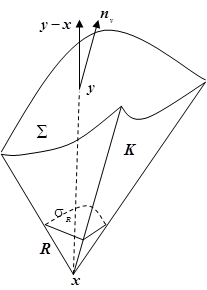
\includegraphics[]{{../img/24-1}.png}
\end{figure}

\begin{definition}
	\textit{Тілесним кутом спостереження} поверхні $\Sigma$ з деякої точки $x \in \RR^3$ будемо називати величину
	\begin{equation}
		\omega(x, \Sigma) = \frac{\sigma_R}{R^2}.
	\end{equation}
\end{definition}

Остання величина, очевидно, не залежить від радіусу сфери $R$ і тому представляє міру тілесного кута. \medskip

У випадку, коли поверхня $\Sigma$ є такою, що величина $\cos(\vec n_y, y - x)$ змінює свій знак в залежності від положення точки $y$, для визначення тілесного кута спостереження такої поверхні, вона розбивається на окремі частини $\Sigma = \bigsqcup_i \Sigma_i$, на кожній з яких $\sign(\cos(\vec n_y, y - x)) = \const$, $y \in \Sigma_i$. \medskip

Таким чином
\begin{equation}
	\omega(x, \Sigma) = \Sum_i \omega(x, \Sigma_i) \cdot \left. \sign(\cos(\vec n_y, y - x)) \right|_{y \in \Sigma_i}.
\end{equation}

\begin{lemma}
	Для будь-якої кусково-гладкої поверхні $\Sigma$, кут спостереження цієї поверхні визначається за формулою
	\begin{equation}
		\omega(x, R) = -\Iiint_\Sigma \frac{\partial}{\partial \vec n_y} \frac{1}{|x - y|} \diff S_y.
	\end{equation}
\end{lemma}

\begin{theorem}[про обмеженість кута спостереження для скінченої поверхні Ляпунова]
	\label{th:4.8.5}
	Якщо $\Sigma$ --- скінченна поверхня Ляпунова, то існує така постійна $C_0$, що
	\begin{equation}
		\label{eq:4.8.61}
		\Iiint_\Sigma \left| \frac{\partial}{\partial \vec n_y} \frac{1}{|x - y|} \right| \diff S_y \le C_0.
	\end{equation}
\end{theorem}

\end{document}
\end{figure}

Для вище наведеної синтаксичної діаграми відповідні множини будуть:
\begin{equation}
    \text{First}_1(\alpha_1 \alpha_2 \ldots \alpha_p A_i) \oplus_1 \text{Follow}_1(A_i) = L_1 = \left\{a_1^1, a_1^2, \ldots, a_1^{n_1}\right\}
\end{equation}
Відповідний фрагмент програми мовою С матиме вигляд:
\begin{verbatim}
extern int lexem_code;
extern char lexem_text[];
void A_i(void) {
    while (
        lexem_code == code_a_1_1 ||
        lexem_code == code_a_1_2 ||
        ... ||
        lexem_code == code_a_1_n_1
    ) {
        ...  // фрагмент програми для слова w
    }
}  // кінець підпрограми для нетермінала A_i
\end{verbatim}

Виконавши аналіз варіантів побудови синтаксичного аналізатора на основі синтаксичних діаграм, покажемо вигляд основної --- main-про\-гра\-ми:
\begin{verbatim}
int lexem_code;
char lexem_text[1<<8];
int main () { 
    get_lexem();
    axiom();  // процедура, пов'язана з аксіомою S граматики
}
\end{verbatim}

\subsection{Контрольні запитання}

\begin{enumerate}
	\item Який граф називається синтаксичною діаграмою?
	\item Як на синтаксичній діаграмі позначаються термінали і нетермінали?
	\item Як на синтаксичній діаграмі позначаються прості (без $\vert$) і складені (з $\vert$)  правила?
	\item Напишіть фрагмент коду (наприклад на мові С) для обробки терміналів і нетерміналів.
	\item Напишіть фрагмент коду (наприклад на мові С) для обробки простих (без $\vert$) і складених (з $\vert$) правил.
	\item Як на синтаксичній діаграмі позначаються правила вигляду $A \mapsto \omega \mid \varepsilon$?
	\item Напишіть фрагмент коду (наприклад на мові С) для обробки правил вигляду $A \mapsto \omega \mid \varepsilon$.
\end{enumerate}
